\documentclass[11pt]{article}
\usepackage[T1]{fontenc}
\usepackage[utf8]{inputenc}
\usepackage{lmodern}
\usepackage[margin=1.08in]{geometry}
\usepackage{amsmath,amssymb,amsthm,mathtools,mathrsfs,bm}
\usepackage{microtype}
\usepackage{graphicx,booktabs,array,enumitem,placeins}
\usepackage{tikz,tikz-cd}
\usetikzlibrary{arrows.meta,calc,decorations.markings,positioning,fit}
\usepackage[numbers,sort&compress]{natbib}
\usepackage[colorlinks=true,linkcolor=blue!45!black,citecolor=blue!45!black,urlcolor=blue!45!black]{hyperref}
\usepackage[capitalise,nameinlink,noabbrev]{cleveref}
\hypersetup{pdftitle={Finite generation for the K(n)-local sphere},pdfauthor={OpenAI}}
\renewcommand{\bibsection}{\section*{\refname}\addcontentsline{toc}{section}{\refname}}
\ifdefined\pdfinfoomitdate\pdfinfoomitdate=1\fi
\ifdefined\pdftrailerid\pdftrailerid{}\fi
\ifdefined\pdfsuppressptexinfo\pdfsuppressptexinfo=15\fi
\newtheorem{theorem}{Theorem}[section]
\newtheorem{lemma}[theorem]{Lemma}
\newtheorem{proposition}[theorem]{Proposition}
\newtheorem{corollary}[theorem]{Corollary}
\newtheorem{conjecture}[theorem]{Conjecture}
\theoremstyle{definition}
\newtheorem{definition}[theorem]{Definition}
\newtheorem{remark}[theorem]{Remark}
\newtheorem{example}[theorem]{Example}
\numberwithin{equation}{section}
\newcommand{\kk}{k}
\newcommand{\Fp}{\mathbb F_p}
\newcommand{\Zp}{\mathbb Z_p}
\newcommand{\Qp}{\mathbb Q_p}
\newcommand{\Cp}{\mathbb C_p}
\newcommand{\Cflat}{C^\flat}
\newcommand{\C}{\mathbb C}
\newcommand{\Z}{\mathbb Z}
\newcommand{\Q}{\mathbb Q}
\newcommand{\R}{\mathbb R}
\newcommand{\N}{\mathbb N}
\newcommand{\cO}{\mathcal O}
\newcommand{\cF}{\mathcal F}
\newcommand{\cL}{\mathcal L}
\newcommand{\cts}{\mathrm{cts}}
\newcommand{\ctensor}{\widehat{\otimes}}
\newcommand{\RGamma}{\mathbf R\Gamma}
\newcommand{\RHom}{\mathbf R\operatorname{Hom}}
\newcommand{\Rlim}{\mathop{\mathbf R\!\varprojlim}}
\DeclareMathOperator*{\colim}{colim}
\DeclareMathOperator{\id}{id}
\DeclareMathOperator{\Fr}{Fr}
\DeclareMathOperator{\Cartier}{C}
\DeclareMathOperator{\Hom}{Hom}
\DeclareMathOperator{\End}{End}
\DeclareMathOperator{\Ext}{Ext}
\DeclareMathOperator{\Tor}{Tor}
\DeclareMathOperator{\Spec}{Spec}
\DeclareMathOperator{\Spf}{Spf}
\DeclareMathOperator{\Spa}{Spa}
\DeclareMathOperator{\GL}{GL}
\DeclareMathOperator{\Gal}{Gal}
\DeclareMathOperator{\Aut}{Aut}
\DeclareMathOperator{\Lie}{Lie}
\DeclareMathOperator{\Ind}{Ind}
\DeclareMathOperator{\Coind}{Coind}
\DeclareMathOperator{\Res}{Res}
\DeclareMathOperator{\Pro}{Pro}
\DeclareMathOperator{\Perf}{Perf}
\DeclareMathOperator{\coker}{coker}
\DeclareMathOperator{\im}{im}
\DeclareMathOperator{\rk}{rk}
\DeclareMathOperator{\rank}{rank}
\DeclareMathOperator{\tr}{tr}
\DeclareMathOperator{\Tr}{Tr}
\DeclareMathOperator{\res}{res}
\DeclareMathOperator{\supp}{supp}
\DeclareMathOperator{\ord}{ord}
\DeclareMathOperator{\length}{length}
\DeclareMathOperator{\ad}{ad}
\allowdisplaybreaks[2]
\setlist{topsep=4pt,itemsep=2pt,parsep=0pt}
\setlength{\emergencystretch}{1em}


\ifdefined\pdfglyphtounicode
\pdfglyphtounicode{tfm:lmex10/parenleftbig}{0028}
\pdfglyphtounicode{tfm:lmex10/parenrightbig}{0029}
\pdfglyphtounicode{tfm:lmex10/parenleftBig}{0028}
\pdfglyphtounicode{tfm:lmex10/parenrightBig}{0029}
\pdfglyphtounicode{tfm:lmex10/parenleftBigg}{0028}
\pdfglyphtounicode{tfm:lmex10/parenrightBigg}{0029}
\pdfglyphtounicode{tfm:lmex10/bracketleftbig}{005B}
\pdfglyphtounicode{tfm:lmex10/bracketrightbig}{005D}
\pdfglyphtounicode{tfm:lmex10/bracketleftbigg}{005B}
\pdfglyphtounicode{tfm:lmex10/bracketrightbigg}{005D}
\pdfglyphtounicode{tfm:lmex10/braceleftBigg}{007B}
\pdfglyphtounicode{tfm:lmex10/bracerightBigg}{007D}
\pdfglyphtounicode{tfm:lmex10/vextendsingle}{23D0}
\pdfglyphtounicode{tfm:lmex10/circleplustext}{2A01}
\pdfglyphtounicode{tfm:lmex10/circleplusdisplay}{2A01}
\pdfglyphtounicode{tfm:lmex10/circlemultiplydisplay}{2A02}
\pdfglyphtounicode{tfm:lmex10/summationtext}{2211}
\pdfglyphtounicode{tfm:lmex10/summationdisplay}{2211}
\pdfglyphtounicode{tfm:lmex10/producttext}{220F}
\pdfglyphtounicode{tfm:lmex10/productdisplay}{220F}
\pdfglyphtounicode{tfm:lmex10/uniontext}{22C3}
\pdfglyphtounicode{tfm:lmex10/uniondisplay}{22C3}
\pdfglyphtounicode{tfm:lmex10/intersectiontext}{22C2}
\pdfglyphtounicode{tfm:lmex10/intersectiondisplay}{22C2}
\pdfglyphtounicode{tfm:lmex10/coproductdisplay}{2210}
\pdfglyphtounicode{tfm:lmex10/hatwide}{0302}
\pdfglyphtounicode{tfm:lmex10/tildewide}{0303}
\pdfglyphtounicode{tfm:lmex10/bracelefttp}{23A7}
\pdfglyphtounicode{tfm:lmex10/braceleftmid}{23A8}
\pdfglyphtounicode{tfm:lmex10/braceleftbt}{23A9}
\pdfglyphtounicode{tfm:lmex10/bracerighttp}{23AB}
\pdfglyphtounicode{tfm:lmex10/bracerightmid}{23AC}
\pdfglyphtounicode{tfm:lmex10/bracerightbt}{23AD}
\pdfglyphtounicode{tfm:lmex10/braceex}{23AA}
\fi

\makeatletter
\AtBeginDocument{%
  \let\kn@theorem@refstepcounter@optarg\refstepcounter@optarg
  \patchcmd{\kn@theorem@refstepcounter@optarg}
    {\cref@old@refstepcounter}{\Hy@theorem@refstepcounter}
    {}{\PackageError{kn-theorem-anchors}
      {Could not patch the optional theorem counter}
      {Review the installed hyperref and cleveref definitions.}}%
  \patchcmd{\cref@thmoptarg}
    {\refstepcounter}{\kn@theorem@refstepcounter@optarg}
    {}{\PackageError{kn-theorem-anchors}
      {Could not patch the shared-counter theorem handler}
      {Review the installed hyperref and cleveref definitions.}}%
  \patchcmd{\cref@thmnoarg}
    {\refstepcounter}{\Hy@theorem@refstepcounter}
    {}{\PackageError{kn-theorem-anchors}
      {Could not patch the ordinary theorem handler}
      {Review the installed hyperref and cleveref definitions.}}%
}
\makeatother

\title{Finite generation for the \texorpdfstring{$K(n)$}{K(n)}-local sphere}
\author{OpenAI}
\date{September 24, 2026}
\begin{document}
\maketitle
\begin{abstract}
We prove that the homotopy groups of the $K(n)$-local sphere are finitely
generated $\mathbb Z_p$-modules in every integer degree, for every prime $p$
and positive height $n$. Equivalently, the same conclusion holds after
$K(n)$-localizing any finite $p$-local spectrum. This answers the degreewise
finiteness question of Hovey and Hovey--Strickland.
\end{abstract}
\tableofcontents
\clearpage
\part{The finiteness problem and continuous coefficients}\label{part:coefficients}
\section{Introduction}\label{sec:introduction}

Let $p$ be a prime, let $K(n)$ denote Morava $K$-theory of height
$n\geq 1$ at $p$, and let $S_p^\wedge$ be the $p$-completed sphere.
Morava localization isolates a single chromatic height in stable
homotopy theory. Even for the sphere, the localized spectrum is not connective, and
a degreewise finiteness statement
must control each integer degree without a connectivity assumption.
The degreewise finite-generation question asks whether each of these
groups is a finitely generated $\Zp$-module. We prove
that it is, at every prime and positive height.

\begin{theorem}\label{thm:main}\label{thm:descent-integral}
For every prime $p$, every integer $n\geq 1$, and every integer $t$,
the $\Zp$-module
\[
                 \pi_t L_{K(n)}S_p^\wedge
\]
is finitely generated. Equivalently, for every finite $p$-local
spectrum $F$, the module $\pi_t L_{K(n)}F$ is finitely generated
over $\Zp$ in every integer degree $t$.
\end{theorem}

The equivalence in the statement follows from finite cofiber sequences,
suspensions, and retracts: finite generation over the Noetherian ring
$\Zp$ is preserved by kernels, cokernels, and extensions. The proof
of the sphere assertion is completed in \cref{sec:sphere}.
There is no uniform bound asserted on the number of generators or on
the order of the torsion as $p$, $n$, or $t$ varies.

\subsection{History and relation to earlier work}
\label{sec:history}

\Cref{thm:main} answers positively the degreewise finite-generation
question stated by Hovey--Strickland \citep[Problem~16.2]{hoveyStrickland1999}
and in Hovey's Morava $K$- and $E$-theory problem list
\citep[Problem~1]{hoveyProblems}.
In Li's terminology, the question asks whether the local sphere is of
\emph{finite type}: its homotopy groups are finitely generated over $\Zp$
in every integer degree \citep[Introduction]{liFiniteType2021}.

The classical height-one calculation expresses the local sphere as the
fiber of an Adams operation on completed $K$-theory
\citep[\S\S1--2]{hopkinsKOne}; we recall the all-degree answer at odd
primes in \cref{prop:sphere-height-one}.
At height two and $p\geq5$, Hovey--Strickland's analysis of Shimomura's
calculations proves that $\pi_aL_{K(2)}F$ is finite for every finite
torsion spectrum $F$ and every integer $a$
\citep[\S15.2 and Theorem~15.1]{hoveyStrickland1999}.
Applied to the Moore spectrum, this supplies the mod-$p$ finiteness
criterion for the sphere in that range. The proof here establishes
that criterion uniformly in the prime and height.

Devinatz approached integral finiteness through continuous homotopy
fixed points for smaller subgroups of the Morava stabilizer. He used
\emph{essentially finite rank}, a condition of finite generation over
the periodicity ring after quotienting by the closure of periodicity
torsion \citep[\S4]{devinatzHomotopy2007}. For Morava $E$-theory $E_n$
and certain closed procyclic stabilizer subgroups $H$, he proved
this property for $\pi_*(E_n^{hH}\wedge F)$ under chromatic-acyclicity
and annihilation hypotheses on the finite spectrum $F$
\citep{devinatzFiniteness2008}.
Such intermediate fixed-point spectra require their own finiteness
condition; these results are distinct from degreewise finite
generation for the full local sphere.

Barthel--Schlank--Stapleton--Weinstein determined the rational answer
at every prime and height \citep[Theorem~A]{bssw2024}:
\[
 \Q\otimes_{\Z}\pi_*L_{K(n)}S
 \cong \Lambda_{\Qp}(\zeta_1,\ldots,\zeta_n),
 \qquad |\zeta_i|=1-2i.
\]
Their coefficient comparison also gives a split injection from
Witt-vector cohomology into degree-zero Lubin--Tate coefficient
cohomology whose complement in each cohomological degree is killed
by a power of $p$
\citep[Theorem~B]{bssw2024}.
These conclusions do not bound the size of integral torsion: the compact
module $\prod_{j\geq1}\Fp$ has zero rationalization and exponent $p$,
but is not finitely generated over $\Zp$.
The present theorem proves that the torsion subgroup is finite in
each integer homotopy degree.
Combined with the rational calculation, it determines the free ranks
in \cref{cor:sphere-ranks}.

Continuous Morava descent links coefficient cohomology to sphere
homotopy \citep[Theorem~1 and Appendix~A]{devinatzHopkins2004}.
The Hopkins--Ravenel smash product theorem, in the descendability
formulation of Mathew, gives a horizontal vanishing line at a finite
page \citep[Corollary~4.4, Theorem~4.18 and Proposition~10.10]{mathew2016}.
Heard states the resulting strongly convergent local Adams spectral
sequence at every prime and height, with a finite-page bound
independent of the input spectrum
\citep[Theorem~4.6 and Proposition~4.13]{heard2023}.
Consequently, finite coefficient cohomology for the Moore spectrum
is enough to obtain finite homotopy in each degree. Establishing that
coefficient finiteness is the main task of this paper.

Our geometric argument places Lubin--Tate deformation theory and
Strauch's torsion strata \citep{lubinTate1966,strauch2007} in the
geometry of the Fargues--Fontaine curve \citep{farguesFontaine2018}.
Scholze--Weinstein relate $p$-divisible groups and their universal
covers to sections of associated bundles \citep{scholzeWeinstein2013}; the relative bundle
and cohomology results used here are those of Fargues--Scholze
\citep{farguesScholze2021}.
The Banach--Colmez theory initiated by Colmez \citep{colmez2002}
was related to coherent sheaves on the curve by Le Bras
\citep{lebras2018}. Ansch\"utz--Le~Bras's relative full-faithfulness
theorem supplies the passage from the compatible linear morphisms
of section sheaves constructed below to bundle maps in families
\citep[Corollary~3.11]{anschutzLeBras2025}.
Within this framework, \cref{sec:completed-tower,sec:kummer,sec:independent-tuples}
construct the marked quotient on each height stratum and its
compact-support comparisons, retaining the marking actions and the
directions of the support limits.

The passage from geometric supports back to compact coefficients
also uses analytic-group duality. Lazard's theory and the formulation
of Beaudry--Goerss--Hopkins--Stojanoska provide the uniform-subgroup
resolutions and their orientation data \citep{lazard1965,bghs}.
The tensor-induction method, recalled by Symonds in its profinite
form, passes from an open subgroup to a complex with finite isotropy
\citep[Theorem~5.2]{symonds2007}.
In \cref{sec:continuous}, trace-one elements for these finite
stabilizers replace averaging by their orders. This permits the
complete-step coefficient comparisons and full-group norm argument
even when the stabilizer has $p$-torsion.

The transfer argument combines classical constructions with a
uniformity problem at finite marking level. Cartier's $p$-basis
construction identifies differential forms with Frobenius-twisted
de Rham cohomology \citep[\S3, Theorem~1]{cartier1957}; we use the
inverse-linear operator in the conventions of Blickle--B\"ockle
\citep[Definition~2.1 and Example~2.23]{blickleBockle2011}.
Lipman's formal residue transformation law gives the finite-root
comparison \citep[Lemmas~(7.2)(b) and~(7.3)]{lipmanResidues1984}.
The additional work is to control the poles of all transfer iterates
and to choose one finite marking level for all sufficiently high
transfers. These are the steps that return the geometric finiteness
statement to the compact coefficient modules
(\cref{sec:transfers,sec:laurent,sec:cutoff,sec:pro-transfer}).

Degreewise finite generation does not extend to every invertible
$K(n)$-local spectrum.
At height two and $p\geq5$, Hovey--Strickland's analysis of
$p$-adically graded spheres gives invertible spectra that are not of
finite type \citep[Theorem~15.1]{hoveyStrickland1999}; Li classifies
the finite-type invertibles in this range
\citep[Theorem~4.22]{liFiniteType2021}.
Thus arbitrary invertible or dualizable local spectra cannot replace
the finite spectra in \cref{thm:main}.
The proof makes no chromatic splitting assumption, and it does not
compute the finite torsion summands or the chromatic fracture maps.


\subsection{The coefficient theorem}

Fix a height $n$ formal group over a sufficiently large finite field
$\kk$ of characteristic $p$. Let $E_n$ be its Morava $E$-theory and
let $P_n$ be its ordinary stabilizer group. The algebraic conclusion
that drives the proof is
\begin{equation}\label{eq:intro-coefficients}
 H^a_{\cts}\bigl(P_n;(E_n)_{2t}/p\bigr)
 \quad\text{is finite for every }a\geq0\text{ and }t\in\Z.
\end{equation}
Here the coefficients have their compact deformation-parameter
topology. The proof retains a precise larger class: integer powers of
the periodicity line tensored with functions on whole finite tuples of
division points, with specified Frobenius-powered coordinates, and
finite sums, tensor products, equivariant summands, and finite
filtrations of these modules. Its exact definition is
\cref{def:mark-coefficients}; its finiteness theorem and Morava
consequence are \cref{thm:coeff-finite,cor:coeff-morava}.
Using whole division-point schemes allows restriction to a deeper
height stratum and descent through finite marking covers. The assertion
is about this class, rather than arbitrary semilinear finite free
modules.

Here is why this coefficient theorem suffices for the sphere.
The finite Galois quotient from $P_n$ to the extended stabilizer
$\mathbb G_n$ preserves degreewise finiteness, including when its
order is divisible by $p$. Morava descent for the Moore spectrum
$S/p$ then has finite second-page entries. A horizontal vanishing
line on a finite page leaves only finitely many of them in each
limiting stem, so $\pi_*L_{K(n)}(S/p)$ is finite in each degree.
Finally, positive-height locality gives derived $p$-completeness.
The finite $p$-power cofibers present each integral homotopy group
as a compact $\Zp$-module with finite quotient modulo $p$; compact
Nakayama proves finite generation. These steps are proved in
\cref{sec:sphere}. The horizontal bound concerns a later page of
the descent spectral sequence; finite mod-$p$ cohomological
dimension of the full stabilizer is not needed.

\subsection{The open-stratum argument}

Write
\[
 A_m=\kk[[u_m,\ldots,u_{n-1}]],\qquad
 B_m=A_m[u_m^{-1}]\quad(1\leq m<n),\qquad A_n=\kk.
\]
We prove coefficient finiteness by downward induction from $A_n$.
At the step indexed by $m$, put $x=u_m$ and $G=P_n$.
The next-height hypothesis makes the cohomology of every finite
boundary strip $x^aM/x^bM$ finite. Thus localization from a compact
allowed coefficient $M$ to $M[1/x]$ has countable kernel and
cokernel on cohomology. It remains to prove that open-stratum
cohomology is countable: the original coefficient cohomology will
then be compact Hausdorff and countable, hence finite. This explains why an
intermediate countability theorem can prove a finiteness theorem.

We work first on finite covers $B_U$ of $B_m$ that mark the
connected formal group and the \'etale Tate module. The index $U$
is an open subgroup of the two marking groups. The finite cover
is an idempotent summand of a localized whole finite free model
$A'[1/x]$. Keeping the whole model before localization ensures
that its boundary layers remain in the next-height coefficient
class. For a suitable compact lattice $\mathcal P=x^{-D}A'$, set
\[
 M^i_U=H^i_\cts(G,\mathcal P),\qquad
 X^i_U=H^i_\cts(G,B_U).
\]
The central task is countability of $X^i_U$ at every sufficiently
deep \emph{fixed} marking level. A statement only after taking the
union of all marking levels would not suffice for the return to
compact coefficients.

The completed marking tower provides the geometric input.
Its quotient by $G$ is the space of independent $r$-tuples in
$H^1(\cO(-1/m))$ on the relative Fargues--Fontaine curve, where
$\cO(-1/m)$ has rank $m$ and degree $-1$, and $r=n-m$. Uniform Kummer calculations and deletion of dependent
tuples make the equivariant compact-support cohomology finite.
A separate ordinary-function calculation shows that invariant
algebraic functions on the tower are constants. This permits a
single normalization of a Cartier transfer $S$ on $B_U$ at one
finite marking stage. Its pole estimate divides the pole order
by a fixed power of $p$, up to a fixed additive loss; consequently
$\mathcal P$ can be chosen $S$-stable and eventually contains the
transfer iterates of every bounded-pole lattice.

To use the compact-support result, we express it as a Laurent
module $W$ of convergent series with fractional $p$-power
exponents, for which every $H_i(G,W)$ is finite over $\kk$.
Residues identify
its quotient by the subspace $W_+$ of positive-$x$-order series
with the discrete transpose transfer tower:
\[
 W/W_+\simeq
 \colim\bigl(\mathcal P^\vee\xrightarrow{S^\vee}
                   \mathcal P^\vee\xrightarrow{S^\vee}\cdots\bigr).
\]
Here $\mathcal P^\vee$ is the continuous $\kk$-linear dual.
The positive-order kernel is homologically acyclic. Its homology
is countable; an analytic-subgroup argument using the Baire
property then makes boundaries open in each complete cycle space, and
absolute Frobenius contracts each positive-order cycle into that
open subgroup. Invertibility of Frobenius then makes the original
cycle a boundary. Compact duality gives
\[
 I^i_U=\bigcap_{a\geq0}S^aM^i_U\quad\text{finite}.
\]
Thus geometry controls a stable transfer image. It has not yet
controlled all of $X^i_U$.

The remaining argument uses the finite translation representations
of the generator-lift torsor. For $m>1$ their distribution algebra
is the regular local ring
$\Lambda=\kk[[D_1,\ldots,D_d]]$, with $d=(m-1)r$.
Exact pro-completion first shows that consecutive transfer images
stabilize modulo countable spaces on a marking tail. Together
with the next-height boundary comparison, this upgrades the
compact result to finiteness of
\[
 F^i_U=\bigcap_{a\geq0}
       \im\bigl(S^aM^i_U\longrightarrow X^i_U\bigr).
\]
Suppose some $X^i_U$ remained uncountable at arbitrarily deep
levels, and choose the highest such degree $b$; the finite-isotropy
bound makes this possible. A top Koszul extension then gives a
finite-diagram operation from degree $b-d$ on a fixed root cover
to degree $b$ on $B_U$, with countable cokernel. One common marking
shrink makes that operation factor through every sufficiently
high transfer. These factorizations use coinduced diagrams of
one fixed self-extension, whose boundary operator has bounded
pole loss. Modulo a countable quotient, the source classes of
the top operation have positive-order cocycle representatives.
Powering these representatives eventually absorbs that pole
loss, so their images belong to every late compact
transfer image and hence to $F^b_U$. The operation therefore has
countable image as well as countable cokernel, contradicting the
choice of $b$. For $m=1$, a Cartier splitting of Frobenius
replaces the top extension and gives the same conclusion directly.

This is the bridge from geometric finiteness to ordinary
coefficient cohomology. \Cref{sec:finite-markings,sec:completed-tower}
construct the finite models and identify the tower;
\cref{sec:kummer,sec:independent-tuples} prove its two geometric
outputs. The transfer and Laurent models are developed in
\cref{sec:transfers,sec:laurent}, and
\cref{sec:cutoff,sec:pro-transfer} prove the stable-image and
fixed-level countability assertions just described.
\Cref{sec:coefficients} extends countability to the allowed
coefficient class, descends the finite marking cover, and closes
the height induction. The continuous-cochain framework used
throughout is established first in \cref{sec:continuous}.

The geometric completion enters through compact supports and the
transpose transfer tower. Compact supports, neighborhood germs,
and supports shrinking to a closed locus use different directions
of passage; \cref{fig:support-directions} displays their maps and
the cohomology that survives. These distinctions permit the
argument to return to an individual algebraic marking level.

\subsection{Conventions}

Throughout the coefficient argument, $\kk$ is finite. It may be
enlarged by a finite extension to define the Honda models and their
endomorphisms. We write $G=P_n$ and reserve $\mathbb G_n$ for the
extended stabilizer in \cref{sec:sphere}. All group cohomology is
continuous, with the topological coefficient conventions of
\cref{sec:continuous}. Compact lattices carry their adic topology;
localized coefficients use continuous cochains with a bounded
denominator. Group homology is denoted by $H_i$ and cohomology by
$H^i$.

For analytic arguments, $C=\Cp$ and $\Cflat$ is its tilt. If
$\mathcal D$ is a compact profinite parameter space, write
$R_{\mathcal D}=C(\mathcal D,\Cflat)$ for its continuous-function
ring. Statements of finiteness with parameters mean finiteness
over $R_{\mathcal D}$. The coefficient-only Frobenius $\varphi$
fixes monomial exponents; the absolute Frobenius $\Fr$ also scales
them. These two operations are distinguished throughout.

We use cohomological grading for complexes. A limit over shrinking
supports, a colimit of restrictions defining a germ, and a colimit
of corestrictions over expanding supports are specified separately
whenever they occur.

\section{Continuous coefficients and full-group duality}
\label{sec:continuous}

The coefficient modules below include compact formal lattices, their
localizations, and spaces of convergent Laurent series.  We first specify
one cochain convention that applies to all three. Finite free resolution
terms make the cohomology of compact coefficients compact Hausdorff;
this is the input used when countability is upgraded to finiteness.
The marked Laurent support module needs a second conclusion: duality
between its group homology and cohomology for the full ordinary
stabilizer. For that module, trace-one elements for finite subgroups
replace averaging by their orders and permit the full-group duality
argument below. The two conclusions have different hypotheses; only
the second requires the trace condition. In this section $\kk$ is a
finite field of characteristic $p$, and $G$ is a compact $p$-adic
analytic group.

\begin{definition}[Complete steps]
\label[definition]{def:cts-steps}
A coefficient module with complete steps is a vector space
$M=\bigcup_{a\geq 0}M_a$, where the $M_a$ are complete Hausdorff linearly
topologized $\kk$-spaces and the inclusions are continuous injections.
The inclusions need not induce the topology on the smaller space.  An
action of $G$ is required to have the following property: for every $a$
there is a $b$ for which $G M_a\subset M_b$ and
$G\times M_a\longrightarrow M_b$ is continuous.  Morphisms satisfy the
analogous condition with no group variable.  We use the bounded-step
continuous cochains
\[
 C^j_{\cts}(G,M)=\colim_a C_{\cts}(G^j,M_a)
\]
with the usual inhomogeneous differential.  Their cohomology is denoted
$H^j(G,M)$.  The same convention applies to continuous functions on any
compact profinite parameter space $\mathcal D$: its complete steps are
$C_{\cts}(\mathcal D,M_a)$ with the topology of uniform convergence.
\end{definition}

All subsequent assertions about these coefficient modules refer to this
specified complex; they do not replace an algebraic image by its closure.
Finite-dimensional discrete modules and compact modules are special
cases.  A localization of a finite module over
$\kk[[x,y_1,\ldots,y_s]]$ has the steps $x^{-a}M_0$, with their adic
topologies.  Laurent modules have the complete steps specified in
\cref{sec:laurent}.

\begin{lemma}[Exact cochains]
\label[lemma]{lem:cts-exact}
Consider an exact sequence of underlying vector spaces
\[
 0\longrightarrow M'\xrightarrow{\iota}M\xrightarrow{q}M''
 \longrightarrow0
\]
whose maps and actions respect complete steps.  Suppose that:
\begin{enumerate}[label=\textup{(\roman*)}]
\item a bounded-step continuous map from a compact profinite space to
      $M$ with image in $\iota(M')$ is bounded-step continuous as a map to
      $M'$;
\item for every compact subset $T$ of a step of $M''$, there is a
      continuous map $s:T\to M_b$ into one step of $M$, with $qs=\id_T$.
\end{enumerate}
Then the corresponding sequence of continuous cochain complexes is
short exact.  In particular, it has the usual long exact cohomology
sequence.  These hypotheses hold for strict short exact sequences of
compact $\kk$-spaces, for short exact sequences of finite modules over a
complete Noetherian local $\kk$-algebra with finite residue field, and
for their localizations with the lattice steps just described.
\end{lemma}

\begin{proof}
The kernel assertion is (i).  A cochain in the quotient has compact
image $T$ in a single step, and composing it with the section in (ii)
lifts that cochain.  The section is not required to commute with $G$.
Thus every degree of the cochain sequence is exact.

For compact vector spaces, continuous duality with discrete vector
spaces turns a strict surjection into an injection.  Splitting that
injection as a map of vector spaces and dualizing gives a continuous
$\kk$-linear section.  In the Noetherian local case the modules are
compact.  A submodule is closed, and its induced topology is its adic
topology by Artin--Rees.  This proves (i), while the compact splitting
proves (ii).  For a localization, a fixed quotient lattice is the image
of a compact source lattice: choose lifts of finitely many module
generators and a common denominator.  Its map from that source lattice
is a strict compact surjection and has a continuous linear section.
The kernel in a fixed lattice is again a finite module, so Artin--Rees
gives (i) after a common enlargement of the denominator.  This also
proves the assertions for finite twists and finite direct sums.
\end{proof}

\begin{lemma}[Compact envelopes and comparison]
\label[lemma]{lem:cts-comparison}
Let $M$ satisfy \cref{def:cts-steps}.
\begin{enumerate}[label=\textup{(\roman*)}]
\item Every compact subset of a step of $M$ is contained in a compact
      $G$-stable $\kk$-subspace $N$ lying in one complete step.  The
      action on $N$ is continuous.  These $N$ form a filtered system
      whose union is $M$, and
      \[
       C^\bullet_{\cts}(G,M)
       =\colim_N C^\bullet_{\cts}(G,N).
      \]
\item The ring $\kk[[G]]$ is Noetherian, and the trivial compact module
      $\kk$ has a resolution $P_\bullet$ by finitely generated free
      compact $\kk[[G]]$-modules.  It may be unbounded.  The comparison
      map
      \[
       \Hom_{\kk[[G]],\cts}(P_\bullet,M)
          \simeq C^\bullet_{\cts}(G,M)
      \]
      is a natural quasi-isomorphism.  Every term on the left is a
      finite power of $M$.
\item A right resolution by finitely generated free compact modules
      similarly defines
      $H_i(G,M)$.  For compact $M$, cohomology and homology computed
      this way are compact Hausdorff, and continuous duality
      interchanges homology and cohomology, with the contragredient
      action on $M^\vee=\Hom_{\cts}(M,\kk)$.
\end{enumerate}
For $G=\Zp$ with generator $\gamma$, the cochain complex is
$[M\xrightarrow{\gamma-1}M]$ in degrees $0,1$.
\end{lemma}

\begin{proof}
Let $T\subset M_a$ be compact.  The set $GT$ is compact in some $M_b$.
Let $N$ be its closed linear span there.  Modulo any open linear
subspace of $M_b$, the image of $GT$ is finite.  Since $\kk$ is finite,
its linear span in that discrete quotient is finite as well.  Thus
$N$ is totally bounded and complete, hence compact.  For any $g\in G$,
the action map $M_b\to M_c$ is continuous after enlarging $c$ uniformly
in $g$.  The image of $N$ in the Hausdorff space $M_c$ is compact and
closed.  It contains the image of the linear span of $GT$, and
continuity therefore shows $gN\subset N$.  The injection $N\to M_c$
is a homeomorphism onto its image, so the restricted action is
continuous.  A finite sum of such spaces is again compact in a common
step.  Every element, and every compact cochain image, is contained in
one of them.  A map from a compact domain whose image lies in $N$ is
continuous into $N$, by its subspace topology in $M_b$.  This proves
(i), including the assertion about cochains.

Choose a normal uniform open subgroup $K\subset G$.  For the
augmentation filtration of $\kk[[K]]$, the associated graded ring is
a polynomial ring on $\dim G$ variables.  Thus $\kk[[K]]$ is
Noetherian, and the finite crossed-product extension $\kk[[G]]$ is
Noetherian as well.  Successively resolving the finitely generated
kernels of a finite free presentation gives $P_\bullet$.  For a
compact module $N$, compare it with the compact bar resolution.
Its terms are induced from compact $\kk$-spaces and are projective:
every compact $\kk$-space is projective by continuous linear duality,
and completed induction preserves that lifting property.
Both are projective resolutions, and their augmentations and
acyclic kernels split as compact $\kk$-spaces by continuous duality.
The lifting construction for resolutions gives chain maps and chain
homotopies in the compact category.  Applying continuous Hom gives
the usual continuous bar cochains.  For comparison with the
ind-profinite formulation under its countability hypotheses, see
\citet[Proposition~8.2 and Corollary~8.4]{boggiCorobCook}.
The compact splitting argument just given does not impose
second countability on $N$ and proves that all its comparison
homotopies are continuous.

There is a well-defined $\kk[[G]]$-action on $M$: integrate on a compact
$G$-stable envelope of a given element.  It is independent of that
envelope.  Since every $P_j$ is finite free, its Hom into $M$ is the
filtered union of its Hom into the $N$.  Filtered colimits of vector
spaces are exact.  Passing the compact comparison and its homotopies
through this colimit proves (ii); in particular no new completion is
introduced.  The same argument applies to the finite free right
resolution and tensor products.  For compact $N$, every differential
has compact, hence closed, image in a finite power of $N$.
Continuous duality is exact on compact vector spaces and takes these
finite-power complexes to the corresponding dual complexes.  This
proves (iii).  Finally,
$\kk[[\Zp]]=\kk[[\gamma-1]]$, and multiplication by $\gamma-1$ gives
the stated two-term free resolution.
\end{proof}

We next make the finite-isotropy hypothesis explicit.  Its verification
for the geometric coefficient algebras will be given in
\cref{prop:mark-finite-isotropy}.

\newpage
\begin{definition}[Trace elements]
\label[definition]{def:cts-trace}
Let $A$ be a commutative $\kk$-algebra with a $G$-action.  A semilinear
$A$-module $M$ with complete steps is trace-admissible if, for every
finite subgroup $F\subset G$, there is $t_F\in A$ satisfying
\[
       \sum_{f\in F}f(t_F)=1,
\]
and multiplication by $t_F$ carries each complete step continuously
into some complete step.  The action is semilinear in the sense that
$g(am)=g(a)g(m)$.
\end{definition}

We will need an elementary local fact about the finite stabilizers of
profinite spaces.  The characteristic-zero Lie group in its proof is
the group $K$, even though the coefficient field has characteristic
$p$.

\begin{lemma}[Equivariant local sections]
\label[lemma]{lem:cts-local-section}
Let $K$ be a normal uniform open subgroup of $G$, and let $X$ be a profinite
$G$-space on which $K$ acts freely.  Suppose that $X\to Y=K\backslash X$
has a continuous $K$-equivariant trivialization as a principal
$K$-space.  Put $H=G/K$.  If $x\in X$ and $y$ is its image, the finite
group $G_x$ maps isomorphically to $H_y$.  There is an $H_y$-invariant
clopen neighborhood $V$ of $y$ and a section $s:V\to X$, with $s(y)=x$,
which is equivariant for $G_x\simeq H_y$.
\end{lemma}

\begin{proof}
An element of $H_y$ has a lift taking $x$ into its $K$-orbit.  Correcting
that lift by the unique element of $K$ gives an element fixing $x$.
Since $K$ acts freely, the resulting homomorphism $G_x\to H_y$ is
bijective.  Write $F=G_x$.  A continuous section with value $x$ at $y$
exists by the assumed trivialization.  Its failure to be $F$-equivariant
is a continuous nonabelian cocycle
$c_f\in C(V,K)$ for the action combining conjugation by $F$ and its
action on $V$.  All $c_f(y)$ equal $1$.  Shrinking to an $F$-invariant
clopen neighborhood makes all these cocycles arbitrarily close to $1$.

Here is the required small-cocycle argument, including the case
$p\mid |F|$.  Choose an $F$-stable sufficiently small Lie lattice in
$\Lie(K)$ on which exponential, logarithm, and the
Campbell--Hausdorff formula converge.  In the Banach space of continuous
functions on $V$ with values in $\Lie(K)$, use the supremum norm of an
$F$-invariant norm.  Put $\lambda_f=\log c_f$ and
$\epsilon=\max_f\|\lambda_f\|$.  Convergence of the
Campbell--Hausdorff series gives, for a fixed constant $c$, the bound
\[
 \|\lambda_{fg}-\lambda_f-f\lambda_g\|\leq c\epsilon^2.
\]
With $b=|F|^{-1}\sum_f\lambda_f$, summing this identity over $g$
gives
\[
 \|\lambda_f+fb-b\|\leq c|\,|F|\,|_p^{-1}\epsilon^2,
 \qquad \|b\|\leq |\,|F|\,|_p^{-1}\epsilon.
\]
Changing the section by $\exp(-b)$ changes its cocycle to
$\exp(-b)c_f f(\exp b)$.  Another application of the same convergence
estimate bounds the new logarithms by $c'\epsilon^2$, for a constant
$c'$ depending only on $F$ and the chosen Lie lattice.  Choose the
initial neighborhood small enough that these exponentials stay in
the convergence lattice and $c'\epsilon<1$.  Iteration then gives
uniformly convergent continuous changes of section, since the
successive logarithms tend to zero at least quadratically.  The limit
has trivial cocycle.  Every change is the identity at $y$, so the
limiting section still takes $y$ to $x$.  Division by $|F|$ was only
performed in $\Qp$; its fixed norm loss was absorbed in the initial
choice of neighborhood.
\end{proof}

\begin{proposition}[A uniform finite-isotropy bound]
\label[proposition]{prop:cts-isotropy-bound}
Fix a normal uniform open subgroup $K\subset G$, and put
$d_G=\dim G$ and $a_G=[G:K]$.  If $M$ is trace-admissible, then
\[
                 H^j(G,M)=0\qquad(j>a_Gd_G).
\]
The same bound holds for $M\otimes_\kk V$ for every finite-dimensional
continuous $G$-representation $V$.  Neither the bound nor the choice
of $K$ depends on $M$ or $V$.
\end{proposition}

\begin{proof}
First consider a finite subgroup $F$ and a semilinear module $L$ with
a trace element $t=t_F$.  The map
\[
 L\longrightarrow \kk[F]\otimes_\kk L,
 \qquad v\longmapsto\sum_{f\in F}f\otimes t f^{-1}v
\]
is $F$-linear when $F$ acts on the first factor of the target.  Its
composite with $f\otimes v\mapsto fv$ is multiplication by
$\sum_f f(t)=1$.  Thus $L$ is a direct summand of an induced module.
The same formulas on continuous cochains, which are finite sums of
bounded continuous operators, show $H^{>0}(F,L)=0$ in our convention.
They apply also to continuous function modules with pointwise
multiplication by $t$, and to any finite-dimensional twist.

The trivial $\kk[[K]]$-module has a finite free resolution of length
$d_G$.  For finite cohomological dimension and uniform-group Poincare
duality, see \citet[Chapter~V, Proposition~2.5.7.1 and
Theorem~2.5.8]{lazard1965} and \citet[Lemma~4.15 and
Proposition~4.16]{bghs}.  Thus $\kk$ has projective dimension $d_G$,
and the Noetherian local ring $\kk[[K]]$ has finitely generated
free terms in a minimal resolution.  A sufficiently deep uniform
subgroup is used also when $p=2$.
Tensor-induce this resolution from $K$ to $G$:
take its completed tensor product over the $a_G$ cosets and let $G$
permute the factors, using the usual signs of complexes and the
conjugate $K$-actions.  Denote the resulting augmented complex by
$T_\bullet\to\kk$.  It is concentrated in degrees $0$ through
$a_Gd_G$.  The original augmented resolution is split exact as a
complex of compact $\kk$-spaces.  Its tensor product is therefore
again a split resolution of $\kk$ in that category.  This is the
tensor-induction construction of
\citet[Theorem~5.2]{symonds2007}.

Each term of $T_\bullet$ is a finite sum of signed permutation modules
$\kk[[X]]$.  Here $X$ is a finite disjoint union of products of copies
of $K$, one for each tensor factor.  The diagonal $K$-action is free,
and setting the first coordinate equal to $1$ gives a continuous
trivialization of $X\to K\backslash X$.  A possible sign is a
locally constant rank-one coefficient and will be carried along.
We claim that
\begin{equation}
 H^j\bigl(G,\Hom_{\kk,\cts}(\kk[[X]],M)\bigr)=0\quad(j>0).
 \label{eq:cts-permutation-acyclic}
\end{equation}
The Hom module is $C_{\cts}(X,M)$, with complete uniform-convergence
steps.  A $K$-trivialization identifies it, after untwisting the
diagonal action on $M$, with a continuously coinduced $K$-module.
Evaluation in the first coordinate contracts the coinduced bar
complex, so its positive $K$-cohomology vanishes.  All operators in
that contraction are bounded continuous operators on function
steps.  The Hochschild--Serre double complex therefore reduces its
$G$-cohomology to the cohomology of $H=G/K$ on the $K$-invariants.

Apply \cref{lem:cts-local-section} at a point of $Y=K\backslash X$.
After shrinking its neighborhood $V$ further, its translates by
elements outside $H_y$ are disjoint: first separate $y$ from the
finitely many distinct points $hy$, and then intersect the resulting
clopen neighborhoods.  On the induced neighborhood $HV$, the
$K$-invariant functions are induced from $H_y\simeq G_x$ acting on
$C_{\cts}(V,M)$, with its possible rank-one sign.  The equivariant
section makes this the ordinary semilinear action on values together
with the action on $V$.  Its higher $H_y$-cohomology vanishes by the
trace-element splitting.  These induced neighborhoods cover the
compact space $Y$.  Choose a finite such cover and take successive
differences of its $H$-invariant clopen members to obtain a disjoint
finite invariant clopen partition.  Each piece retains its local
description and splitting.  Finite additivity and finite-group
Shapiro now prove \eqref{eq:cts-permutation-acyclic}.

Finally form the first-quadrant double complex
\[
 C^u_{\cts}\bigl(G,\Hom_{\kk,\cts}(T_v,M)\bigr).
\]
The compact $\kk$-linear contracting homotopy of the augmented
$T_\bullet$ acts on these Hom modules: a continuous map from a
compact domain into a step has image in a compact envelope, so
integration and the contracting homotopy take place in complete
steps by \cref{lem:cts-comparison}.  Computing first in the $v$
direction identifies the total cohomology with $H^*(G,M)$.
Computing first in the $u$ direction and using
\eqref{eq:cts-permutation-acyclic} leaves only $u=0$ and
$0\leq v\leq a_Gd_G$.  This proves the bound.  Tensoring $M$ with
$V$ preserves every step condition and the trace elements, so the
same construction proves the last assertion with the identical
bound.
\end{proof}

The preceding bound is deliberately larger than the dimension.
It is its uniformity under finite twists that permits passage from
torsion-free open subgroups to the full group, including at primes
where $G$ has torsion.

\begin{proposition}[Full-group duality]
\label[proposition]{prop:cts-full-duality}
Assume that the orientation character of $G$ is trivial over $\kk$.
For every trace-admissible $M$ there are natural isomorphisms
\[
                  H_i(G,M)\simeq H^{d_G-i}(G,M)
                  \qquad(i\in\Z).
\]
Here homology is zero in negative degrees, and cohomology is zero in
negative degrees.  In particular $H^j(G,M)=0$ for $j>d_G$.
The ordinary stabilizer $P_n$ has trivial orientation character and
$d_G=n^2$, so this assertion applies to it without a twist.
\end{proposition}

\begin{proof}
Write $R=\kk[[G]]$, $R_K=\kk[[K]]$, $H=G/K$, and
$\Sigma=\kk[H]$.  Regard $\Sigma$ as the quotient bimodule of $R$.
It is perfect as a left or right $R$-module, since it is induced
from the length-$d_G$ free resolution over $R_K$.  Uniform-group
duality, with its conjugation action retained, gives
\begin{equation}
 \RHom_R(\Sigma,R)\simeq\Sigma[-d_G]
 \label{eq:cts-bimodule-duality}
\end{equation}
as a $(\Sigma,R)$-bimodule.  To recall the equivariance in this
formula, restrict $R$ to $R_K$ and decompose it into its finitely
many cosets.  The dual of the uniform resolution has cohomology
only in degree $d_G$, with one orientation line on each coset.
Right translation permutes those lines by the right regular action;
precomposition by a quotient element gives the left regular action
and its action on the orientation line.  The latter is trivial by
hypothesis.  This proves exactly the two commuting actions asserted
in \eqref{eq:cts-bimodule-duality}.  The uniform duality, orientation
identification, and compatibility with conjugation are also recorded in
\citet[Propositions~4.16 and~4.36, Theorem~4.19 and
Remark~4.23]{bghs}.

Put
\[
 C=\RHom_R(\Sigma,M)=\RGamma(K,M),\qquad
 B=\Sigma\otimes_R^{\mathbf L}M.
\]
Perfectness permits evaluation of the dual resolution against $M$,
so \eqref{eq:cts-bimodule-duality} gives a natural equivalence
$C\simeq B[-d_G]$ in the derived category of $\Sigma$-modules.
The cohomology of $C$ lies in degrees $0,\ldots,d_G$.  The finite
free comparisons in \cref{lem:cts-comparison} show that these
derived expressions compute precisely the specified continuous
cochains and homology, even when $M$ is a union of steps.

We prove that the finite-group norm
\begin{equation}
       \kk\otimes_\Sigma^{\mathbf L}C
           \longrightarrow\RHom_\Sigma(\kk,C)
       \label{eq:cts-finite-norm}
\end{equation}
is an equivalence.  This is the point where finite subgroup
cohomology cannot be discarded.  For any finite-dimensional left
$\Sigma$-module $V$, derived adjunction gives
\[
 \Ext^j_\Sigma(V,C)
       =H^j(G,V^*\otimes_\kk M).
\]
By \cref{prop:cts-isotropy-bound} these groups vanish for
$j>a_Gd_G$, uniformly in $V$.  Choose a bounded-below injective
resolution $J^\bullet$ of $C$.  If $N$ is greater than both $d_G$
and $a_Gd_G$, dimension shifting along its exact tail gives
\[
 \Ext^1_\Sigma(V,\ker(J^N\to J^{N+1}))
       =\Ext^{N+1}_\Sigma(V,C)=0.
\]
Every quotient $\Sigma/I$ by a left ideal is finite-dimensional.
Baer's criterion therefore says that this last kernel is injective.
Truncating there gives a bounded complex of injective modules
representing $C$.

For a finite group algebra, every injective module, including an
infinite-dimensional one, is projective.  Indeed, the canonical
injection of any module $L$ into
$\Hom_\kk(\Sigma,L)$ splits if $L$ is injective; the target is free
because the symmetric pairing on $\kk[H]$ identifies coinduction
with induction.  On a free module of arbitrary rank the ordinary
norm is an isomorphism from coinvariants to invariants: on each
copy of $\kk[H]$ it sends the class of $1$ to $\sum_{h\in H}h$.
It is consequently an isomorphism on projective summands.  Applying
this degreewise to the bounded injective-projective model of $C$
proves \eqref{eq:cts-finite-norm}, with no infinite totalization or
completion.

The left-hand side of \eqref{eq:cts-finite-norm}, shifted by $d_G$,
is
\[
 (\kk\otimes_\Sigma^{\mathbf L}C)[d_G]
       \simeq\kk\otimes_R^{\mathbf L}M;
\]
the right-hand side is $\RGamma(G,M)$.  Taking cohomology in
degree $-i$ of the shifted equivalence gives
$H_i(G,M)=H^{d_G-i}(G,M)$, with the stated grading.

For $G=P_n$, its Lie algebra is the central division algebra
$D_n$ of degree $n$ over $\Qp$.  Conjugation by $a\in D_n^\times$
has determinant
\[
 \det(L_a)\det(R_a)^{-1}
   =\operatorname{Nrd}(a)^n\operatorname{Nrd}(a)^{-n}=1.
\]
The orientation character is the reduction of this determinant
character, hence is trivial.  The dimension of $D_n$ is $n^2$.
\end{proof}

\begin{remark}
For a nontrivial orientation character, the same proof retains its
one-dimensional line in \eqref{eq:cts-bimodule-duality} and gives
the corresponding orientation-twisted duality.  We only use the
untwisted case stated above.  The proposition makes no assertion
that arbitrary $\kk[[G]]$-modules have finite cohomological
dimension: its trace-element hypothesis is essential when $G$
contains $p$-torsion.
\end{remark}

\clearpage
\part{Finite markings and the completed tower}\label{part:tower}
\section{Finite markings and integral models}
\label{sec:finite-markings}

This section provides the finite algebraic data used by both sides of
the proof. The whole models give coefficients whose boundary layers
belong to the next height stratum; their localized summands give the
marking covers whose completed tower is studied geometrically. We also
identify the full division-point lift schemes, because later transfer
maps require their scheme structure and natural group actions.

Fix a prime $p$ and a height $n$.  Choose a finite field $\kk$ containing
the fields of definition of the Honda groups $\Gamma_j$, $1\leq j\leq n$,
and of their endomorphisms.  We use Honda coordinates for which
$[p]_{\Gamma_j}(T)=T^{p^j}$.  In this section
\[
 G=P_n,\qquad
 A_m=\kk[[u_m,\ldots,u_{n-1}]],\qquad 1\leq m\leq n.
\]
The formal group $\cF$ over $A_m$ is the restriction of the universal
deformation of $\Gamma_n$ to the height-at-least-$m$ locus.
The deformation-ring construction is due to
\citet[Proposition~1.1 and Theorem~3.1]{lubinTate1966}; the Honda conventions and
endomorphism structure are recalled in \citet[Appendix~A2.2]{ravenel1986}.  Its finite
division schemes are formed over $A_m$ before any localization.  If
$m<n$, put
\[
 x=u_m,\qquad B_m=A_m[1/x],\qquad r=n-m.
\]
The chosen parameters are successive Hasse coefficients: the ideals of
the deeper height loci are $(u_m,\ldots,u_{j-1})$, and the first
coefficient of $[p]_{\cF}(T)$ over $A_m$ is $xT^{p^m}$; compare
\citet[(1.1) and \S2]{strauch2007}.  Replacing a
parameter by a unit multiple gives the same constructions.

The action of $G$ comes with coordinate changes
$\alpha_g:g^*\cF\longrightarrow\cF$.  Write $\chi_g=\alpha_g'(0)$ and
let $\cL_m$ denote the free rank-one $A_m$-module with this semilinear
action.  Composition of the $\alpha_g$ gives the cocycle identity for
$\chi_g$.  Comparing the leading coefficients of the $p$-series gives
\begin{equation}
 g(x)=\chi_g^{p^m-1}x.
 \label{eq:mark-height-character}
\end{equation}
Thus $\cL_m$ is the periodicity line, up to the immaterial choice of
inverse convention.  All its integer powers will be retained.  All
finite $A_m$-modules below carry their compact topology; localizations
carry the bounded-denominator coefficient convention of
\cref{sec:continuous}.

\subsection{The coefficient class}

Since the $p$-series factors through $T^{p^m}$, its $\ell$-fold iterate
factors through $T^{p^{m\ell}}$.  For $\ell\geq1$ and
$0\leq b\leq m\ell$, define
\[
 D_m(\ell,b)
   =A_m[\,T^{p^b}\,]\ \subseteq\
     A_m[[T]]/([p^\ell]_{\cF}(T)).
\]
The brackets here mean the $A_m$-subalgebra generated by the indicated
element; it will be finite over $A_m$.

\begin{definition}[Allowed coefficients]
\label[definition]{def:mark-coefficients}
The basic coefficients at height $m$ are
\begin{equation}
 \cL_m^{\otimes w}\otimes_{A_m}
       \bigotimes_{j=1}^{s}D_m(\ell_j,b_j),
 \qquad w\in\Z,\quad 0\leq b_j\leq m\ell_j,
 \label{eq:mark-basic-coefficients}
\end{equation}
where $s$ may be zero.  These are functions on whole tuples of division
points, with the indicated powered coordinates; no independence
condition is imposed.  The allowed class $\mathscr C_m$ is their closure
under finite direct sums, tensor products, equivariant direct summands,
and finite equivariant filtrations whose successive quotients belong to
the class.  An extension in this definition is an exact sequence of
compact semilinear $A_m$-modules.
\end{definition}

\begin{lemma}
\label[lemma]{lem:mark-powered-division}
The algebra $D_m(\ell,b)$ is finite free of rank $p^{n\ell-b}$ over
$A_m$.  Its construction and action are intrinsic to relative
Frobenius and commute with restriction to a deeper height locus.
Every member of $\mathscr C_m$ is finite free over $A_m$, and reduction
modulo $x$ sends $\mathscr C_m$ into $\mathscr C_{m+1}$.
\end{lemma}

\begin{proof}
Write $[p^\ell]_{\cF}(T)=f(T^{p^b})$.  Modulo the maximal ideal of
$A_m$, the series $f(Z)$ is $Z^{p^{n\ell-b}}$.  Weierstrass preparation
therefore gives
\[
 f(Z)=v(Z)W(Z),\qquad
 W(Z)=Z^{p^{n\ell-b}}+\sum_{i<p^{n\ell-b}}c_iZ^i,
\]
where $v$ is a unit and all $c_i$ lie in the maximal ideal.  Consequently
$[p^\ell](T)$ generates the same ideal as $W(T^{p^b})$.
Division by this monic polynomial shows both that
$A_m[Z]/(W(Z))\longrightarrow A_m[[T]]/([p^\ell](T))$, $Z\mapsto T^{p^b}$,
is injective and that its image has basis
$1,T^{p^b},\ldots,T^{p^b(p^{n\ell-b}-1)}$.  This proves the rank assertion.

A coordinate change $T\mapsto a(T)$ carries $T^{p^b}$ to
$a(T)^{p^b}$, a series in $T^{p^b}$.  Thus the subalgebra is preserved;
it is the relative Frobenius image of the division scheme on coordinate
rings.  The same monic-division calculation after base change identifies
the resulting algebra with the corresponding powered division algebra
of the restricted group.  In particular it commutes with passage to
$A_{m+1}=A_m/(x)$.  The numerical restriction on $b$ persists, since
$b\leq m\ell\leq(m+1)\ell$.

The basic modules are finite free.  An extension with finite free
quotient splits as an underlying $A_m$-module, so its middle term is
finite free.  A finite direct summand is projective and hence free over
the local ring $A_m$.  These facts also show that reduction modulo $x$
preserves the exact filtrations in the definition.  The periodicity line
restricts to the corresponding line at height $m+1$.  The last assertion
now follows by induction over the finite constructions defining the
class.
\end{proof}

\subsection{Connected jets and whole finite models}

For the remainder of this section assume $m<n$.
Over $B_m$, the connected part of $\cF[p^\infty]$ is a formal group of
height $m$.  Its isomorphisms to $\Gamma_m$ form a pro-finite-\'{e}tale
$P_m$-torsor.  The ring-level assertion used here is
\citet[Lecture~14, Theorem~1]{lurieFormalGroups}: the isomorphism algebra
of two formal group laws of the same exact positive height over a ring
is an increasing union of finite \'{e}tale algebras.  In the present
Honda trivialization its finite quotients can be chosen as follows.

\begin{proposition}[Integral connected-jet models]
\label[proposition]{prop:mark-jets}
For each $h\geq0$, the connected marking through exponent $p^h$ has a
finite free model $H_{m,h}$ over $A_m$.  There are coordinates
$a_0,\ldots,a_h$ and polynomials in earlier coordinates such that
\begin{equation}
\begin{aligned}
 a_0^{p^m-1}&=x,\\
 a_i^{p^m}-x^{p^i}a_i&=P_i(a_0,\ldots,a_{i-1}),
       &&1\leq i\leq h.
\end{aligned}
 \label{eq:mark-jet-equations}
\end{equation}
If the first Hasse coefficient is normalized only up to a unit, the
corresponding unit factors are inserted in these equations.  The
residue monomials
\[
 a_0^{e_0}a_1^{e_1}\cdots a_h^{e_h},\qquad
 0\leq e_0<p^m-1,\quad 0\leq e_i<p^m\ (i>0),
\]
are an $A_m$-basis.  The $G$-action preserves this model and admits a
finite filtration with quotients integer powers of $\cL_m$.  The
filtration remains such a filtration on every deeper height locus.
\end{proposition}

\begin{proof}
Write an isomorphism $f:\cF\longrightarrow\Gamma_m$ as an ordinary
power series.  Its coefficient at $T^{p^i}$ is $a_i$.  At a degree $j$
which is not a power of $p$, some intermediate binomial coefficient
$\binom{j}{v}$ is nonzero modulo $p$.  In the coefficient of
$X^vY^{j-v}$ in
$f(\cF(X,Y))=\Gamma_m(f(X),f(Y))$, the unknown coefficient of $T^j$
therefore has a nonzero constant coefficient.  All other terms involve
earlier coefficients.  It follows inductively that every non-$p$-power
coefficient is a polynomial over $A_m$ in the preceding $a_i$.

Now compare $f([p]_{\cF}(T))$ with $f(T)^{p^m}$.  In degree $p^m$ this
gives $a_0x=a_0^{p^m}$, hence the first equation, since $a_0$ is
invertible on the open marking space.  In degree $p^{m+i}$, the only
term involving $a_i$ on the left is $x^{p^i}a_i$; all remaining terms
involve earlier coefficients.  This proves
\cref{eq:mark-jet-equations}, with polynomials over $A_m$.  The
recursive comparison is also the usual proof of the Honda
classification; see \citet[Theorem~A2.2.12, its proof, and
Lemmas~A2.2.20--A2.2.21]{ravenel1986}.

Let $H_{m,h}$ be the successive monic algebra defined by these
equations.  Monic division gives the displayed basis, so it is finite
free of rank $(p^m-1)p^{mh}$.  After inverting $x$, $a_0$ is invertible,
the derivative of its equation is invertible, and the derivative of
the $i$th subsequent equation is $-x^{p^i}$.  Thus
$H_{m,h}[1/x]$ is finite \'{e}tale.

The actual marking quotient is finite \'{e}tale by the ring-level
classification above.  After a strictly henselian base change its
fiber is the corresponding quotient of $P_m$.  A Honda automorphism
has $p^m-1$ possible nonzero linear coefficients, and $p^m$ choices at
each succeeding $p$-power; the other coefficients are then determined.
This follows either from the Honda coefficient calculation or from
the order filtration on its endomorphism ring.  Hence that quotient
has rank $(p^m-1)p^{mh}$. The equations define a map from
$H_{m,h}[1/x]$ to its coordinate ring. Every jet coefficient is a
polynomial in $a_0,\ldots,a_h$, so these coordinates distinguish
geometric jets. The map on geometric function algebras is therefore
surjective, and finite \'{e}taleness gives surjectivity of the map
itself. A surjection between finite
\'{e}tale algebras of the same rank is an isomorphism, as can be checked
after strict henselization.  This identifies the algebra, including
over nonreduced test bases, with the connected marking quotient.

Precomposing $f$ with $\alpha_g$ gives
\begin{equation}
 g(a_i)=\chi_g^{p^i}a_i+Q_{g,i}(a_0,\ldots,a_{i-1}),
 \qquad g(a_0)=\chi_ga_0.
 \label{eq:mark-jet-triangular}
\end{equation}
Every coefficient in this formula lies in $A_m$; only finitely many
coefficients of $\alpha_g$ are used at a fixed jet order.  The formulas
preserve the defining relations after inverting $x$.  Since
$H_{m,h}$ is $x$-torsion-free, they preserve them before localization
as well.  The inverse coordinate change supplies the inverse action.

Order the displayed basis lexicographically starting with $e_h$, then
$e_{h-1}$, and so on.  In expanding a transformed monomial, any use of
an earlier-variable term in \cref{eq:mark-jet-triangular} lowers this
order.  Reducing a power $a_i^{p^m}$ by its monic equation lowers it
again.  The diagonal term on a basis vector is therefore
$\chi_g^{e_0+pe_1+\cdots+p^he_h}$.  The initial spans in this order are
stable, with the claimed line quotients.  All these spans and
quotients are free over $A_m$, so the filtration specializes exactly
to every deeper height locus.  Finally the formulas are continuous
in $g$ and in the compact coefficient topology, because every fixed
finite coefficient quotient uses finitely many coefficients of the
continuous universal coordinate change.
\end{proof}

On the same open, marking the \'{e}tale Tate module gives a
$\GL_r(\Zp)$-torsor.  Its action commutes with changes of connected
marking and with $G$.  Put
\[
 J=P_m\times\GL_r(\Zp).
\]
We use a cofinal sequence of normal product congruence subgroups
$U\subset J$.  The connected factors can be chosen among the kernels
of the jet quotients just constructed: the subsequence corresponding
to $1+p^a\cO_{D_m}$ is cofinal.  After omitting finitely many terms,
both factors, and hence $U$, are uniform and torsion-free.  Let $B_U$
denote the finite \'{e}tale $J/U$-torsor algebra of the two markings.

\begin{proposition}[A whole model for a finite marking]
\label[proposition]{prop:mark-whole-model}
For each such $U$ there are a finite free $A_m$-algebra $A'$, with
integral multiplication laws in a fixed basis, and a $G$-invariant
idempotent $e\in B'=A'[1/x]$ such that
\[
 B_U=eB',\qquad B'/B_m\text{ is finite \'{e}tale}.
\]
As a semilinear $A_m$-module, $A'$ has a finite filtration whose
quotients are basic coefficients in $\mathscr C_m$.  Its reduction
modulo $x$ has such a filtration in $\mathscr C_{m+1}$.
In a whole basis $A'=\bigoplus_\nu A_m b_\nu$, the $G$-action is
given by continuous matrices over $A_m$.  The base action is a
continuous formal action preserving $(x)$; in particular the
whole-basis action has a uniform pole bound, including for compact
families of group elements.
\end{proposition}

\begin{proof}
Choose the connected jet order $h$ and the \'{e}tale level $\ell$
defining $U$.  Relative Frobenius of exponent $m\ell$ kills precisely
the connected part of $\cF[p^\ell]$ on the exact-height open.  Its
image is the \'{e}tale quotient, whose coordinate algebra is
$D_m(\ell,m\ell)[1/x]$.  One can check \'{e}taleness directly: writing
$[p^\ell](T)$ in the variable $Z=T^{p^{m\ell}}$, its linear coefficient
is invertible when $x$ is invertible.  Equivalently its geometric
fibers have $p^{r\ell}$ distinct points, and the resulting finite
flat group scheme is \'{e}tale.

The set of ordered bases in the $r$-fold power of this finite
\'{e}tale group is an open and closed subscheme.  Indeed it can be
checked after an \'{e}tale trivialization of the group, where it is a
subset of a finite constant set.  Its characteristic idempotent is
preserved by every isomorphism of the group, in particular by $G$.
Take
\[
 A'=H_{m,h}\otimes_{A_m}D_m(\ell,m\ell)^{\otimes r}
\]
and extend that idempotent over the connected factor.  This gives
the asserted $e$ and the identification with the two marking
torsors.  Both factors of $B'$ are finite \'{e}tale over $B_m$.

Tensor the monomial filtration of \cref{prop:mark-jets} with the whole
powered tuple algebra.  Its quotients are precisely of the form
\cref{eq:mark-basic-coefficients}.  The same holds after reduction
modulo $x$ by \cref{lem:mark-powered-division}.  Tensoring the finite
free bases gives a basis of $A'$, and all multiplication constants
lie in $A_m$.  This construction uses the entire tuple algebra at
the boundary; no extension or specialization of $e$ across $x=0$
is involved.

The base action and the action on a powered division coordinate
are substitution by the universal formal coordinate change and
its appropriate Frobenius power.  Their reduction in a fixed
finite free basis converges in the parameter topology.  Modulo
any power of the maximal ideal, only a finite truncation is
needed, so its matrix entries vary continuously in $g$.  The
connected-jet entries have the same property by
\cref{eq:mark-jet-triangular}.  Thus all matrices have integral
entries and zero pole loss in the whole lattice, uniformly in
$g$.  Preservation of $(x)$ is \cref{eq:mark-height-character}.
\end{proof}

\subsection{Generator lifts and roots}

At full markings the schemes of lifts of the ordered \'{e}tale
generators are torsors under the connected division groups.  Their
inverse limit is a torsor for
\[
 T=\varprojlim_{[p]}\Gamma_m[p^\ell]^r.
\]
Here $T$ and its finite quotients are affine group schemes; their
representations below are coactions of the coordinate Hopf algebras.
The two marking groups act on this description by changing the two
bases; $G$ commutes with the resulting translations.

\begin{proposition}[The lift algebras are root algebras]
\label[proposition]{prop:mark-roots}
At level $\ell$, the reduced closure over $A_m$ of lifted geometric
\'{e}tale bases has coordinate algebra
\[
 R_{m,\ell}=\kk[[t_{1,\ell},\ldots,t_{r,\ell}]].
\]
If $s_i=t_{i,\ell}^{p^{m\ell}}$, the intermediate algebra generated
by the $s_i$ over $A_m$ is
\[
 S_{m,\ell}=\kk[[s_1,\ldots,s_r]],\qquad
 A_m\subseteq S_{m,\ell}.
\]
After inverting $x$, $S_{m,\ell}[1/x]$ is the \'{e}tale basis algebra,
and $R_{m,\ell}[1/x]$ is its full generator-lift algebra.  In
particular the latter is the root extension of order $p^{m\ell}$,
finite free of rank $p^{m\ell r}$, with no reduction of the lift
scheme omitted.  These identifications are natural under the $G$
action, changes of markings, and finite \'{e}tale base change.
For $j\leq\ell$, earlier division coordinates are integral series
in the $p^{m(\ell-j)}$ powers of the level-$\ell$ coordinates.
In particular the base parameters, in first-level coordinates,
have order at least $p^m$.
\end{proposition}

\begin{proof}
Strauch describes the corresponding torsion stratum over the completed
maximal unramified coefficient base.  There the full Drinfeld
level-$p^\ell$ deformation ring $\widetilde R_\ell$ is finite flat
over the Lubin--Tate deformation ring and regular, with the universal
torsion coordinates $\phi_1,\ldots,\phi_n$ as regular parameters.
The quotient
\[
 \widetilde R_\ell/(\phi_1,\ldots,\phi_m)
\]
is a regular ring of dimension $r$ over the height-at-least-$m$
base; its generic torsion coordinates $\phi_{m+1},\ldots,\phi_n$
give the lifted \'{e}tale bases.  The induced generic Galois action
is the full $\GL_r(\Z/p^\ell)$ action
\citep[\S3, Proposition~4.1, and the proof of Theorem~2.1]{strauch2007}.
Over our finite Honda field we establish the whole reduced closure
directly, using the division divisor.

Let $C_\ell$ be the coordinate algebra of the whole $r$-fold division
tuple scheme over $A_m$.  Over $B_m$, let $Q_\ell$ be the finite
\'{e}tale algebra of ordered bases of the \'{e}tale division group,
and let $L_\ell$ be its full generator-lift algebra.  The map
$Q_\ell\to L_\ell$ is finite faithfully flat: its fibers are torsors
under the product of the $r$ connected division groups.  The basis
condition selects an open and closed subscheme of the powered tuple
scheme, so $C_\ell[1/x]\to L_\ell$ is surjective.  Define
\[
 R=\operatorname{image}\bigl(C_\ell\longrightarrow (L_\ell)_{\mathrm{red}}\bigr).
\]
This is the reduced closure of the entire lifted basis locus.  It is
finite over $A_m$, as a quotient of $C_\ell$, and
$R[1/x]=(L_\ell)_{\mathrm{red}}$.  Every component dominates $B_m$:
the finite flat algebra $L_\ell/B_m$ has its minimal primes over the
generic point.  Taking their closures adds no vertical component.
Consequently $A_m\to R$ is injective and integrality gives $\dim R=r$.
The closed fiber of $C_\ell$ is supported at the tuple of origins, so
$R$ is complete local with residue field $\kk$.
Denote the universal lifted
coordinates by $t_i=t_{i,\ell}$, and put
$t_{i,1}=[p^{\ell-1}]_{\cF}(t_i)$.  At geometric generic points, the
$p^r$ combinations of the $t_{i,1}$ are all the points of
$\cF[p]$, each with multiplicity $p^m$.  Weierstrass preparation
therefore gives the divisor identity
\begin{equation}
 [p]_{\cF}(Z)
  =v(Z)\prod_{a\in\Fp^r}
       \left(Z-\sum_{i=1}^{r}{}_{\cF}[a_i](t_{i,1})\right)^{p^m}
       \quad\text{in }R[[Z]],
 \label{eq:mark-basis-divisor}
\end{equation}
where $v$ is a unit.  Equality holds in $R$, since $R$ is reduced and
all its components meet the generic basis locus.  Modulo $(t_1,\ldots,t_r)$,
the right side is a unit times $Z^{p^n}$.  Successively comparing the
Hasse coefficients forces every $u_m,\ldots,u_{n-1}$ to vanish in
that quotient.  Consequently the maximal ideal of $R$ is generated
by the $r$ elements $t_i$.  Completeness gives a surjection
$\kk[[T_1,\ldots,T_r]]\twoheadrightarrow R$.  A nonzero ideal of
the power-series domain has quotient of dimension at most $r-1$;
since $\dim R=r$, the kernel is zero.  This proves the asserted
description of $R_{m,\ell}$ over $\kk$.

For the powered assertion, set $h=p^{m\ell}$ and let
$S=A_m[s_1,\ldots,s_r]\subset R$, where $s_i=t_i^h$.  This is a
finite $A_m$-module: it is a submodule of a finite module over the
Noetherian ring $A_m$.  It is therefore complete; it is local with
residue field $\kk$, and $\dim S=r$ by integrality.  The first-level
coordinates raised to $p^m$ belong to $S$.  Indeed,
$[p^{\ell-1}](T)$ is a series in $T^{p^{m(\ell-1)}}$, so raising
$[p^{\ell-1}](t_i)$ to $p^m$ gives an integral series in $s_i$.
The same is true of all their formal-group combinations.

To apply \cref{eq:mark-basis-divisor} inside $S$, write
$[p]_{\cF}(Z)=V(Z^{p^m})$.  The monic factor on its right is a
polynomial in $Z^{p^m}$ whose coefficients lie in $S$.  Division of
$V(W)$ by this monic polynomial in $W$ is performed in $S[[W]]$;
the remainder is zero after embedding in $R[[W]]$, hence is already
zero in $S[[W]]$.  The quotient is a unit, as its reduction at the
closed point is a unit.  Reducing now modulo $(s_1,\ldots,s_r)$
again gives a unit times $W^{p^r}$.  The successive Hasse
coefficients therefore put all the base parameters in $(s_1,\ldots,s_r)S$.
Thus $S$ is complete with maximal ideal generated by the $r$
elements $s_i$.  The dimension argument just used gives
$S=\kk[[s_1,\ldots,s_r]]$.  In particular the inclusion of the base
factors through this power-series subring.

The powered coordinates on the exact-height open are the \'{e}tale
division coordinates.  Their basis condition gives a surjection
$Q_\ell\to S[1/x]$, since the $s_i$ generate the target over $B_m$.
The composite into $R[1/x]=(L_\ell)_{\mathrm{red}}$ is injective:
$Q_\ell$ is reduced, and the faithfully flat map
$Q_\ell\to L_\ell$ cannot send a nonzero element of $Q_\ell$ to
a nilpotent.  Thus $Q_\ell\simeq S[1/x]$, identifying the basis
algebra on the whole open.

The extension
\[
 \kk[[s_1,\ldots,s_r]]\ \longrightarrow\
 \kk[[t_1,\ldots,t_r]],\qquad s_i\longmapsto t_i^h,
\]
is free with basis $\prod_i t_i^{e_i}$, $0\leq e_i<h$; this follows
by partitioning the monomials in a power series by their exponents
modulo $h$.  Its rank is $h^r$.  After localization, $R[1/x]$ is a
closed subscheme of the generator-lift scheme over $S[1/x]$.  That
lift scheme is a torsor under the product of $r$ connected
$p^\ell$-division groups, so it too is finite locally free of rank
$p^{m\ell r}=h^r$.  On coordinate rings this is a surjection of
finite locally free modules of equal rank, hence an isomorphism.
This proves the assertion about the full scheme, including its
nonreduced geometric fibers.

All maps used to define $s_i$ are relative Frobenius maps, and all
transition maps are multiplication by powers of $p$.  They commute
with group isomorphisms.  Changing a basis replaces the $t_i$ by
formal integral linear combinations, whose $h$th powers are the
corresponding combinations of the $s_i$.  Hence the descriptions
are natural for $G$ and both marking actions.  For an \'{e}tale
algebra, relative Frobenius is an isomorphism
\cite[Lemma~41.14.3, Tag~0EBS]{stacks}.  Root extension therefore
commutes with any subsequent finite \'{e}tale marking extension:
if $E/S[1/x]$ is \'{e}tale, then
\[
 E\otimes_{S[1/x]}R[1/x]\simeq E^{1/h}.
\]
The same identity gives descent through marking levels, with their
natural change-of-marking actions retained.  Finally
$t_{i,j}=[p^{\ell-j}](t_{i,\ell})$ is an integral series in
$t_{i,\ell}^{p^{m(\ell-j)}}$ with coefficients in $A_m$.
Substituting the already proved expressions for those coefficients
puts it in
$\kk[[t_{1,\ell}^{p^{m(\ell-j)}},\ldots,
 t_{r,\ell}^{p^{m(\ell-j)}}]]$.
At level one, each base parameter lies in the maximal ideal of
$\kk[[t_{1,1}^{p^m},\ldots,t_{r,1}^{p^m}]]$, which gives the stated
order bound.
\end{proof}

\begin{lemma}[Basic coefficients on the marked torsor]
\label{lem:mark-associated-coefficients}
At full markings, each basic coefficient in
\cref{eq:mark-basic-coefficients} is associated to a finite-dimensional
translation representation over $\kk$.  Its torsor, representation,
and maps descend to finite marking levels, with the natural
change-of-marking actions.  A fixed finite collection of such data
admits a common sufficiently deep level.  The periodicity line
already trivializes at the linear connected jet.
\end{lemma}

\begin{proof}
Choose a level $L$ at least as large as all the $\ell_j$.  A lift
of the marked \'{e}tale generators in $\cF[p^L]$ supplies a splitting
of the connected--\'{e}tale extension at that level: send a standard
basis vector of $(\Z/p^L)^r$ to its lift and extend by the group
law.  The lifts are $p^L$-torsion, so this is well defined.  The
resulting product decomposition identifies the division group with
\[
 \Gamma_m[p^L]\times(\Z/p^L)^r.
\]
Changing the lifts translates this splitting by
$\Gamma_m[p^L]^r$.  The coordinate algebra of the displayed group
is a finite-dimensional $\kk$-space; its restrictions to the lower
levels and their powered-coordinate images are functorial under
relative Frobenius.  They therefore give finite-dimensional
representations of the same finite translation quotient.  Torsor
descent identifies their associated bundles with the original
powered division coefficients.  Tensor products and finite sums
preserve this identification.

The derivative of the connected marking identifies the intrinsic
linear coefficient line with the Honda line.  This is an
equivariant trivialization and uses only $a_0$, which is invertible
on the open.  It treats every positive or negative periodicity
power.  The schemes and their coactions use finite division level,
finitely many coefficients, and a finite-dimensional vector space
over the finite field $\kk$.  The continuous change-of-marking
action consequently factors through a finite quotient on each
fixed datum.  Finite presentation of the torsor descent and its
maps puts them at a finite marking stage; the maximum of finitely
many stages works for a finite collection.  This assertion is about
the basic coefficients.  Arbitrary extensions and summands in
$\mathscr C_m$ will be handled by exact sequences and retracts,
without asserting that every such extension is itself a constant
translation representation.
\end{proof}

\subsection{Finite isotropy and trace one}

\begin{proposition}[Geometric hypotheses for the isotropy bound]
\label[proposition]{prop:mark-finite-isotropy}
Suppose $U$ is a torsion-free product marking subgroup as above.
Every finite subgroup $F\subset G$ acts geometrically freely on
$\Spec B_U$.  There is an element $a_F\in B_U$ with
\[
 \sum_{f\in F}f(a_F)=1.
\]
Multiplication by $a_F$ is continuous between bounded-denominator
steps of finite coefficient bundles.  It also acts continuously
on bounded analytic section and compact-support models, with
compact profinite parameters retained.  Thus the geometric
coefficient modules satisfy the trace and module-action
hypotheses of \cref{prop:cts-isotropy-bound,prop:cts-full-duality}.
Equivalently they satisfy \cref{def:cts-trace}.
\end{proposition}

\begin{proof}
Let $g\ne1$ have finite order $N$, and suppose it fixes a geometric
point $z$ of $\Spec B_U$.  Its image on the base factors through
\[
 R=A_m/I_g,\qquad I_g=(g(a)-a:a\in A_m).
\]
Every ideal of a Noetherian complete local ring is closed, so $R$
is complete local.  The framing action becomes an actual
automorphism $\gamma$ of the formal group over $R$.  Its reduction
at the closed point is the nonidentity Honda automorphism $g$.
The difference endomorphism
\[
 f(T)=\gamma(T)-_{\cF}T
\]
therefore has nonzero reduction, of some finite order $d$ in $T$.
Weierstrass preparation over $R$ makes
$H=\Spec R[[T]]/(f(T))$ finite free of rank $d$.
For every $\ell$ the fixed subscheme of the finite division scheme is
\[
 H_\ell=\Spec R[[T]]/(f(T),[p^\ell](T)),
\]
a closed subscheme of $H$.  Every geometric fiber of $H_\ell$ thus
has coordinate dimension at most $d$.  This preparation and these
finite quotients were formed over the complete base before
localization.

Lift $z$ to a full marking $t$ over its algebraically closed residue
field.  Such a lift exists by the marking torsors: the inverse
system of nonempty finite fibers has surjective transitions.  As
$g$ fixes the $U$-coset, $gt=tu$ for some $u\in U$.  Commutation
of the actions gives $u^N=1$.  Since $U$ is torsion-free, $u=1$.
In particular $\gamma$ induces the identity on the connected
height-$m$ formal group, hence on its finite $p^\ell$-division
subgroup inside the specialized division scheme.  That subgroup
has rank $p^{m\ell}$ and is contained in $(H_\ell)_z$.  Taking
$p^{m\ell}>d$ is a contradiction.  Notice that only the connected
marking is needed for this last contradiction; no splitting of
the connected--\'{e}tale extension at $z$ is being used.
To spell out the specialization, its connected division coordinate
is nilpotent, so evaluation of each original formal series there
is a finite sum.  It gives a surjection from the specialized
prepared algebra defining $H_\ell$ onto that connected coordinate
algebra, since both $f$ and $[p^\ell]$ vanish there.  This uses only
the finite algebra formed over $R$ and never identifies
$R[[T]]\otimes_R\Omega$ with $\Omega[[T]]$.

We give the trace argument for an arbitrary commutative algebra
$D$ with a geometrically free action of a finite group $F$; this
avoids a finite-type assumption on $B_U$.  Put $C=D^F$.  The image
$I=\Tr_F(D)$ is an ideal of $C$, because trace is $C$-linear.  If
$I$ were contained in a maximal ideal $\mathfrak m$ of $C$, the
integrality of $D/C$ would give a point $z:D\to\Omega$ extending
$C\to\kappa(\mathfrak m)$, for an algebraically closed field
$\Omega$.  Integrality follows directly from the orbit polynomials
$\prod_{f\in F}(T-f(d))$, and the point follows by lying-over.
In $D_\Omega=D\otimes_C\Omega$, consider the surjective
$\Omega$-algebra evaluations
\[
 e_f(d\otimes\lambda)=z(f(d))\lambda,\qquad f\in F.
\]
Geometric freeness says that these maps are distinct.  Their
maximal kernels are therefore distinct, and the Chinese remainder
theorem gives $b\in D_\Omega$ such that
$e_1(b)=1$ and $e_f(b)=0$ for $f\ne1$.  Hence
$e_1(\Tr_F(b))=1$.  On the other hand, writing
$b=\sum_i d_i\otimes\lambda_i$ gives
\[
 \Tr_F(b)=\sum_i\Tr_F(d_i)\otimes\lambda_i=0,
\]
because all $\Tr_F(d_i)$ lie in $\mathfrak m$.  This contradiction
shows that $I=C$.  Thus a single element of $D$ has trace one.
The argument uses no assertion that invariants commute with
residue-field base change.  Apply it with $D=B_U$.

Finally, write $a_F=e x^{-c}a$ in the whole finite model, with
$a\in A'$ and $c$ finite.  Multiplication is a finite matrix over
$B_m$ in the whole basis.  Clearing its finitely many denominators
makes it a continuous map from any compact lattice into a fixed
enlarged lattice.  The same statement holds for finite coefficient
bundles, after choosing lattices.  On an analytic bound where
$x$ is bounded away from zero, the same function and finite
matrices are bounded.  Multiplication is continuous on sections,
preserves supports, and commutes with restriction; it therefore
acts on the section and support complexes.  Retaining a compact
profinite parameter means using the uniform seminorm on that
parameter, so the same bound applies.  These are precisely the
trace-one multiplication and semilinearity conditions in the
cited cohomological propositions.  The additional continuity of
the later Laurent representatives under changes of coordinates
is verified in \cref{lem:laurent-action}.
\end{proof}

\subsection{Boundary strips}

\begin{lemma}[Boundary comparison under the next-height hypothesis]
\label[lemma]{lem:mark-strips}
Assume that $H^i_\cts(G,M)$ is finite for every $M\in\mathscr C_{m+1}$
and every $i\geq0$.  Let $L$ be either a member of $\mathscr C_m$ or
$A'\otimes_{A_m}M$ for $M\in\mathscr C_m$, where $A'$ is a whole
model from \cref{prop:mark-whole-model}.  For any integers $a<b$,
\[
 H^i_\cts(G,x^aL/x^bL)
\]
is finite in every degree.  For each fixed integer $a$, localization
induces a map
\[
 H^i_\cts(G,x^aL)\longrightarrow H^i_\cts(G,L[1/x])
\]
with countable kernel and cokernel.  These assertions concern
whole lattices; they do not require a model for the idempotent
$e$ on the closed locus.
\end{lemma}

\begin{proof}
The quotient $x^aL/x^bL$ has a finite filtration whose layers are
$x^jL/x^{j+1}L$ for $a\leq j<b$.  Multiplication by $x^j$ and
\cref{eq:mark-height-character} identify the $j$th layer with
\[
 (L/xL)\otimes_{A_{m+1}}
       \cL_{m+1}^{\otimes j(p^m-1)}.
\]
If $L\in\mathscr C_m$, this belongs to $\mathscr C_{m+1}$ by
\cref{lem:mark-powered-division}.  For a whole marking model it
has a finite filtration with the same property by
\cref{prop:mark-whole-model}.  The next-height hypothesis and the
long exact cohomology sequences of these finite filtrations prove
finiteness of every strip.

Put $V=L[1/x]/x^aL$.  It is the countable increasing union of the
finite-width strips $x^{a-j}L/x^aL$, $j\geq0$.  With the stipulated
bounded-denominator cochains, its cochain complex is their
filtered colimit.  Filtered colimits of vector spaces are exact,
so its cohomology is the filtered colimit of their finite
cohomology groups.  It is countable, since $\kk$ is finite.  The
short exact coefficient sequence
\[
 0\longrightarrow x^aL\longrightarrow L[1/x]
   \longrightarrow V\longrightarrow0
\]
is exact on continuous cochains by \cref{lem:cts-exact}; in
concrete terms one lifts a cochain through a compact strip after
enlarging its denominator bound.  The long exact sequence
identifies the localization kernel with an image of
$H^{i-1}_\cts(G,V)$ and its cokernel with a subspace of
$H^i_\cts(G,V)$.  Both are countable, as claimed.
\end{proof}

\paragraph{The remaining induction step.}
At $m=n$, the allowed coefficients are finite-dimensional over $\kk$,
so the finite-type resolution of \cref{lem:cts-comparison} gives finite
cohomology in each degree. For $m<n$, assume this finiteness for every
coefficient in $\mathscr C_{m+1}$. The target of
\crefrange{sec:completed-tower}{sec:pro-transfer}
is the marked scalar assertion
\[
 H^i_{\cts}(G,B_{U_\nu})\text{ is countable}
 \qquad(i\geq0,\ \nu\geq\nu_0),
\]
where $(U_\nu)$ is a cofinal decreasing sequence of normal product
congruence subgroups and one $\nu_0$ works for all degrees.
This is \cref{thm:pro-countability}: it concerns each individual
finite marking level on that tail.

The return to arbitrary allowed coefficients still requires
\cref{sec:coefficients}. There the associated translation
representations extend scalar countability to basic coefficients,
and finite marking descent removes the cover. The boundary comparison
above then makes the original compact coefficient cohomology
countable. It is compact Hausdorff by \cref{lem:cts-comparison}, hence
finite. Exact filtrations and summands give the full allowed class,
closing the induction in \cref{thm:coeff-finite}.

\section{The completed tower and its extension-space quotient}
\label{sec:completed-tower}

The finite markings of the preceding section supply an inverse tower
of covers of the exact-height open. Our goal is to identify its quotient
by the ordinary stabilizer with a space of independent extension
classes, including its relative structure, both marking actions, and
its compact supports. That identification is the input for the
cohomological calculations in the next part.

Fix $1\leq m<n$ and put $r=n-m$. Write $x=u_m$ and
$y_i=u_{m+i}$ for $1\leq i<r$. All analytic spaces in this
section are diamonds over $\Spa(C,\cO_C)$, with characteristic-$p$
functions obtained by tilting. We use the perfected analytic domain
\[
 X_m=\{0<|x|<1,\ |y_1|,\ldots,|y_{r-1}|<1\}
\]
associated with $A_m$; here and below an empty list of $y$-coordinates
is permitted. For a finite marking level $U\subset J$, let $Z_U\to X_m$
be the finite \'{e}tale cover obtained from $B_U$. The completed full
marking tower $Z_\infty$ is the inverse limit of these covers in
perfectoid spaces, or equivalently in diamonds. Completion always means
completion for the spectral norms on relatively compact analytic charts.
In particular, no ideal containing the invertible element $x$ is used
as an ideal of completion on $B_m$.
The chart constructions use perfected Tate algebras, rational
localizations, and fiber products of perfectoid spaces
\citep[Proposition~5.20, Theorem~6.3(i)--(ii), and
Proposition~6.18]{scholzePerfectoid2012}.

Write $\mathcal V_j=\cO(1/j)$ for the basic bundle of rank $j$ and
degree one on the Fargues--Fontaine curve. Its section sheaf is denoted
by $\mathcal H_j=H^0(\mathcal V_j)$. We use the Honda model obtained
by reducing the Lubin--Tate formal group over the unramified extension
$F_j/\Qp$ with logarithm
$\sum_{a\geq0}T^{p^{ja}}/p^a$. Its $p$-series is $T^{p^j}$.
The universal cover is a perfected open ball with Honda addition
\citep[Proposition~3.1.3]{scholzeWeinstein2013}.
The following explicit comparison fixes the endomorphism convention
as well as the underlying section sheaf.

\begin{lemma}[The covariant Honda action]
\label[lemma]{lem:tower-honda-action}
The Honda universal-cover sheaf identifies covariantly with
$\mathcal H_j$. This identification intertwines the original rational
Honda endomorphisms with the bundle endomorphisms, preserving
composition. Over a geometric base, it identifies
\[
 D_j:=\End(\mathcal V_j)\simeq\End^0(\Gamma_j),
 \qquad P_j=\cO_{D_j}^{\times}.
\]
The invariant $1/j$ uses the arithmetic-Frobenius convention in the
Honda presentation. The comparison is relative on perfectoid test
bases and is linear over the sheaf $\underline{\Qp}$ of continuous
$\Qp$-valued functions.
\end{lemma}

The relative bundle and section descriptions used below are those of
\citet[Sections~II.2--II.3]{farguesScholze2021}. The coordinate
argument proves the particular partial-height tower comparison,
including its integral frame and support data.

Put
\[
 \mathcal N_m=H^1(\mathcal V_m^{\vee}),\qquad
 (\mathcal N_m^r)_{\mathrm{ind}}
 =\{(\xi_1,\ldots,\xi_r):\xi_1,\ldots,\xi_r
       \text{ are $\Qp$-linearly independent}\}.
\]
Independence is a fiberwise condition defining the indicated open
subfunctor: relations can be normalized in the compact parameter
space $\mathbb P^{r-1}(\Qp)$, so their incidence locus has closed
image under projection. As an additive diamond, after choosing the standard untilt
description,
\begin{equation}\label{eq:tower-additive-model}
 \mathcal N_m\simeq
 \mathbb G_{a,C}^{\diamond}/\underline{F_m},
\end{equation}
where $F_m/\Qp$ is unramified of degree $m$. One obtains this by
expressing $\mathcal V_m^{\vee}$ as the pushforward of $\cO(-1)$
from the curve with coefficient field $F_m$ and applying the untilt-divisor
sequence
$0\to\cO(-1)\to\cO\to i_*C\to0$.
The resulting $H^0$ and $H^1$ sequence is
$0\to\underline{F_m}\to\mathbb G_{a,C}^{\diamond}
\to\mathcal N_m\to0$; the section and vanishing assertions are
\cite[Propositions II.2.3, II.2.5(ii), and II.3.4]{farguesScholze2021}.
This additive description does not choose affine coordinates for the
$P_m$-action: that action is the one on bundle extensions.

\begin{theorem}[Completed tower comparison]\label{thm:tower-comparison}
There is a choice of a fixed determinant-height normalization for which
\begin{equation}\label{eq:tower-quotient}
 [Z_\infty/G]\simeq(\mathcal N_m^r)_{\mathrm{ind}}.
\end{equation}
The map $Z_\infty\to(\mathcal N_m^r)_{\mathrm{ind}}$ is a
$G=P_n$-torsor. The comparison commutes with base change and with both
integral marking actions of
$J=P_m\times\GL_r(\Zp)$. Under the convention that a matrix acts
on a kernel framing by pushout, $(a,b)\in P_m\times\GL_r(\Zp)$
acts on extensions by pullback along $a^{-1}$ on $\mathcal V_m$ and
pushout along $b$ on $\cO^r$.
\end{theorem}

The proof separates three geometric constructions.  The normalized
coordinates first identify the completed tower with only the \'{e}tale
marking as $(\mathcal H_n^r)_{\mathrm{ind}}$
(\cref{lem:tower-etale-comparison}).  Independent sections then give
an exact sequence with quotient of type $\mathcal V_m$, and the
connected marking supplies an actual relative frame of that quotient.
Finally the determinant height selects the integral frame torsors.
We first establish the Honda-action comparison needed to retain the
original groups throughout these constructions.

\begin{proof}[Proof of \cref{lem:tower-honda-action}]
Work on an affinoid perfectoid test base $T=\Spa(R,R^+)$ over $\kk$.
The chosen inclusion $\mathbb F_{p^j}\subset\kk$
induces the unramified field $F_j$ in the relative period coefficients;
Witt Frobenius $\phi$ restricts to arithmetic Frobenius there.
For a topologically nilpotent universal-cover coordinate $X$, the
covariant Lubin--Tate section map is
\begin{equation}\label{eq:tower-honda-period-map}
 \psi_j(X)=\sum_{i\in\Z}p^i[X^{p^{-ji}}].
\end{equation}
Here brackets denote Teichm\"uller lifts. This is the natural additive
isomorphism of \citet[Proposition~II.2.2]{farguesScholze2021}, applied
with coefficient field $F_j$, uniformizer $p$, and residue-field
cardinality $p^j$. Pushforward along the unramified degree-$j$ map
of coefficient-field curves gives
$\cO(1/j)=f_*\cO(1)$, as in the proof of
\citet[Theorem~II.2.14]{farguesScholze2021}. Thus its target is
$\mathcal H_j$, and $\phi^j\psi_j(X)=p\psi_j(X)$.

We record the continuity needed to use this comparison in families.
On a closed period annulus, its Gauss seminorms can be normalized by
$|p|=p^{-1}$ and $|[z]|_s=|z|^s$, with $s$ in a compact interval
$[a,b]$ and $a>0$. On an input chart $\|X\|\leq\rho<1$, the
$i$th term of \eqref{eq:tower-honda-period-map} has norm at most
\[
 p^{-i}\rho^{a p^{-ji}}.
\]
For $i\to+\infty$ the first factor forces convergence. For $i=-h$
the bound is $p^h\rho^{a p^{jh}}$, which also tends to zero.
Both tails converge uniformly on the input chart. The formula is
therefore continuous, commutes with bounded maps of perfectoid
algebras, and glues on test bases. Termwise calculation gives
\[
 \psi_j(X^p)=\phi\psi_j(X),\qquad
 \psi_j(cX)=[c]\psi_j(X)\quad(c\in\mathbb F_{p^j}).
\]
Consequently the Honda Frobenius $\Pi_j:X\mapsto X^p$ and the
Teichm\"uller scalars satisfy, on both sides with the same composition,
\[
 \Pi_j^j=p,\qquad \Pi_j[c]=[c^p]\Pi_j.
\]
These are the Honda algebra relations of
\citet[A2.2.17--A2.2.18]{ravenel1986}. They identify the original
integral endomorphism ring as a finite free $\Zp$-algebra generated
by $\Pi_j$ and a primitive unramified Teichm\"uller root. In
particular finitely many monomials in these generators span it over
$\Zp$. Compatibility with integers extends to $\Zp$ by continuity:
the discrepancy after an approximation modulo $p^h$ has Honda norm
at most $\rho^{p^{jh}}$, and its period-side norm tends to zero on
each annulus. The displayed action identities therefore hold for
the entire original maximal order, and then for its rational division
algebra after inverting $p$.

For the required sheaf linearity, let
$\alpha\in C^0(|T|,\Qp)$ and fix an input section $v$.
Quasicompactness supplies $d\geq0$ such that $b=p^d\alpha$ is
$\Zp$-valued. Choose its finite clopen-constant approximation $b_h$
modulo $p^h$, and write $b-b_h=p^hc_h$, with $c_h$ integral.
Integral Honda scalar operations do not increase the norm, so
\[
 \|[b]v-_{\Gamma_j}[b_h]v\|\leq\rho^{p^{jh}}.
\]
On each fixed period annulus, multiplication by an integral scalar
has norm at most one, and
\[
 \|(b-b_h)\psi_j(v)\|\leq |p|^h\|\psi_j(v)\|.
\]
On each clopen piece constant scalar compatibility gives
$\psi_j([b_h]v)=b_h\psi_j(v)$. Taking the two limits and then
commuting with $p^{-d}$ proves the assertion for $\alpha$ on the
same test base.

Positive-slope vanishing identifies derived sections of
$\mathcal V_j$ with its ordinary section sheaf. Relative full
faithfulness \citep[Corollary~3.11]{anschutzLeBras2025}, with the
just-verified topological-field sheaf convention, turns the Honda
action into a unital, composition-preserving map
$\End^0(\Gamma_j)\to\End(\mathcal V_j)$. Its source is a division
algebra, so the map is injective. Over a geometric base both algebras
have dimension $j^2$
over $\Qp$: for the target, the endomorphism bundle has slope zero
and rank $j^2$, and geometric classification together with
$H^0(\cO)=\Qp$ computes its sections. Thus the map is an
isomorphism. The unique maximal orders correspond, identifying the
actual Honda automorphism group with the bundle-frame group.
Uniqueness in full faithfulness makes this construction compatible
with relative base change. On a general test base the corresponding
action is by the sheaf $\underline{D_j}$ of continuous $D_j$-valued
functions; its global sections need not have finite dimension over
$\Qp$. No opposite action is introduced.
\end{proof}

\subsection{Normalized division coordinates}

Set $q_n=p^n$ and $q_m=p^m$.  We begin with the universal cover of a
fixed deformation over a bounded perfectoid chart.  Here the parameters
$u_i$ are given; later they will themselves be functions of the tuple
of division coordinates.  In a coordinate reducing to the Honda
coordinate, the multiplication series of the universal formal group
$\mathcal F$ satisfies
\begin{equation}\label{eq:tower-series-bounds}
 [p]_{\mathcal F}(T)\equiv T^{q_n}
       \pmod{(u_m,\ldots,u_{n-1})},\qquad
 [p]_{\mathcal F}(T)\in A_m[[T^{q_m}]].
\end{equation}
All coefficients are integral. Thus on a chart on which
$\max |u_i|\leq\lambda<1$, and for inputs of norm less than one,
uniformly on each closed chart of strictly subunit input radius,
\[
 |[p]_{\mathcal F}(s)-s^{q_n}|\leq\lambda,
 \qquad
 |[p]_{\mathcal F}(s)-[p]_{\mathcal F}(t)|
       \leq |s-t|^{q_m}.
\]
The second inequality is a coefficientwise power-series estimate in
the coordinate $T^{q_m}$, so it also holds for uniform norms over a
relative perfectoid affinoid. Every fixed-level series evaluation
converges on its own chart of radius less than one. The coefficientwise
Lipschitz constant is one, independently of that radius, so these
estimates remain uniform when the radii of successive finite
approximants tend to one; the parameter bound $\lambda<1$ stays fixed.

For a compatible division sequence
$[p]_{\mathcal F}t_{j+1}=t_j$, define
\begin{equation}\label{eq:tower-normalized-limit}
 z=\lim_{j\to\infty}t_j^{q_n^j}.
\end{equation}
Consecutive terms differ by at most $\lambda^{q_n^j}$; hence this
limit converges uniformly. Conversely, for $|z|<1$, the formula
\begin{equation}\label{eq:tower-inverse-cover}
 t_j=\lim_{N\to\infty}
       [p]_{\mathcal F}^{N}
          \bigl(z^{1/q_n^{j+N}}\bigr)
\end{equation}
converges uniformly: consecutive approximants differ by at most
$\lambda^{q_m^N}$. The formulas are inverse. Indeed, the difference
between $t_l$ and $z^{1/q_n^l}$ has norm at most $\lambda$, and
applying $[p]^{l-j}$ bounds the difference at level $j$ by
$\lambda^{q_m^{l-j}}$, which tends to zero. This proves both
uniqueness and recovery of a given compatible sequence.  Conversely,
for the sequence constructed from a given $z$, finite telescoping
gives $|t_j-z^{1/q_n^j}|\leq\lambda$, and hence
\[
 |t_j^{q_n^j}-z|\leq\lambda^{q_n^j}\longrightarrow0.
\]
Thus the other composite is the identity as well.  It also shows
that the kernel of projection to $t_0$ is the integral Tate module of
the \'{e}tale part: on a perfect geometric fiber, the connected torsion
has no nonzero points. Projection to $t_0$ is v-locally surjective,
since the monic division equations admit roots after a finite cover
at every level.

We now let the deformation vary with the division tuple.  The whole
reduced closures of \cref{prop:mark-roots} give free polydisc
coordinates at each finite level; this extra input will identify the
completed tower itself.

\begin{lemma}[The analytic \'{e}tale-marking tower]
\label[lemma]{lem:tower-etale-comparison}
Let $Z_\infty^{\mathrm{et}}$ denote the completed perfected tower of
ordered \'{e}tale Tate-module markings over $X_m$.  There is a relative
analytic isomorphism
\[
 Z_\infty^{\mathrm{et}}\simeq(\mathcal H_n^r)_{\mathrm{ind}},
\]
where independence is fiberwise over $\Qp$.  The isomorphism is
equivariant for $G$ and $\GL_r(\Zp)$.  It is the restriction of an
analytic isomorphism from the completed perfected tower of reduced
closures $R_{m,l}$ to the open ball underlying $\mathcal H_n^r$.
\end{lemma}

\begin{proof}
Adjoining the point coordinates to the powered \'{e}tale coordinates
is a pure-root extension by \cref{prop:mark-roots}; it does not change
a perfected analytic level.  Thus these point coordinates compute
the completed \'{e}tale marking tower.  Use first the reduced
level-$l$ closure in \cref{prop:mark-roots}. Its coordinate ring has
regular parameters
$t_{1,l},\ldots,t_{r,l}$. Two consequences of that proposition are
\begin{align}
 u_i&\in k[[t_{1,1}^{q_m},\ldots,t_{r,1}^{q_m}]],
       \quad u_i(0)=0,\label{eq:tower-first-order}\\
 t_{i,j}&=F_{i,j,l}
      (t_{1,l}^{q_m^{l-j}},\ldots,t_{r,l}^{q_m^{l-j}})
       \quad(j\leq l),\label{eq:tower-early-coordinates}
\end{align}
with $F_{i,j,l}$ integral convergent formal series, without a constant
term. Formula \eqref{eq:tower-early-coordinates} follows also by
iterating the second assertion of \eqref{eq:tower-series-bounds}
and expressing the base parameters in the powered level-$l$
coordinates.

For $l\geq1$ and $0<\rho<1$ in the divisible value group, take the closed chart
\[
 X_l(\rho)=
 \{\max_i |t_{i,l}^{q_n^l}|\leq\rho\}
\]
in the perfected generic fiber of this regular ring. If
$\lambda=\max |u_i|$ at a point of this chart, then
\eqref{eq:tower-first-order} and finite telescoping of
\eqref{eq:tower-series-bounds} give
\[
 \lambda\leq\|t_{\cdot,1}\|^{q_m},\qquad
 \|t_{\cdot,1}\|
    \leq\max(\lambda,\rho^{1/q_n}).
\]
If $\lambda>\rho^{1/q_n}$ these inequalities would give
$\lambda\leq\lambda^{q_m}<\lambda$. Therefore
\begin{equation}\label{eq:tower-uniform-parameter}
 \lambda\leq\rho^{q_m/q_n}<1.
\end{equation}
For $y_{i,l}=t_{i,l}^{q_n^l}$ this yields
\begin{equation}\label{eq:tower-normalized-error}
 \|y_{\cdot,l+1}-y_{\cdot,l}\|
   \leq\lambda^{q_n^l}
   \leq\rho^{q_mq_n^{l-1}}<\rho.
\end{equation}
The finite integral injective transition maps are surjective on
these charts. To check the radius condition in this assertion, lift a
point by lying over in the finite map. The bound
\eqref{eq:tower-uniform-parameter} holds at the original point and
therefore at its lift; \eqref{eq:tower-normalized-error} then forces
the lifted normalized coordinate to have norm at most $\rho$.
Consequently pullback on functions is isometric for spectral norms,
also after adjoining all $p$-power roots.

Let $L_\rho$ be the completed direct limit of these perfected
affinoid algebras. The limits $z_i=\lim_l y_{i,l}$ define a map from
the perfected radius-$\rho$ Gauss algebra to $L_\rho$. This map is
isometric. To see this without inferring it from points, take a
polynomial $f$ in finitely many $p$-power roots of the variables. At
every sufficiently late level, $f(y_{1,l},\ldots,y_{r,l})$ has
exactly the radius-$\rho$ Gauss norm of $f$: the $t_{i,l}$ are free
regular polydisc coordinates, and taking powers followed by perfection
does not change the perfected Gauss algebra. These evaluations converge
to $f(z_1,\ldots,z_r)$ in the common spectral norm. The limit has the
same norm, since the differences eventually have smaller norm than a
given nonzero Gauss norm. Completion gives the asserted isometry; its
image is therefore closed.

It is surjective as well. For fixed $i,j$, replace $t_{a,l}$ in
\eqref{eq:tower-early-coordinates} by $z_a^{1/q_n^l}$. The
substituted series converges on the radius-$\rho$ polydisc and the
error is bounded by
\begin{equation}\label{eq:tower-surjectivity-error}
 \lambda^{q_m^{l-j}}
 \leq\rho^{(q_m/q_n)q_m^{l-j}}\longrightarrow0.
\end{equation}
Thus $t_{i,j}$ is in the closed image. Taking any fixed $p$-power
root in this argument merely takes that root of the error bound, so
all perfected finite-level generators are in the image. They are
dense in $L_\rho$, proving surjectivity. This establishes inverse
affinoid morphisms. Varying $\rho$ gives the isomorphism of open
balls.

All the preceding estimates are uniform norm estimates for integral
series. Hence the constructed morphisms commute with bounded base
change, glue on overlapping charts, and apply with any compact
profinite parameter space $\mathcal D$ by using the uniform norm on
$C(\mathcal D,C^\flat)$. In particular they establish a relative
analytic comparison, not just a comparison of geometric points.

The normalized limits respect addition, integral scalar operations,
and the full $G$-action. For example, replace the deformation addition
series by its Honda reduction. Their difference on integral inputs
has norm at most $\lambda$. Transporting to a fixed earlier division
level contracts this error by $q_m^{l-j}$, exactly as in
\eqref{eq:tower-surjectivity-error}. The same argument applies to
the integral coordinate change associated with $g\in G$ and its
Honda reduction; compact families of $g$ have the same coefficient
bounds. It applies also to the finite sums defining integral changes
of an \'{e}tale basis. Thus the comparison is equivariant for $G$
and $\GL_r(\Zp)$, continuously in both groups.

We can now identify the exact-height open. An integral relation among
the normalized sections gives, by the inverse construction, the same
relation among their compatible division sequences: if the normalized
relation is zero, its point at a fixed earlier level is bounded by
$\lambda^{q_m^{l-j}}$ for every $l$, and is zero. The converse follows
by applying the limit formula. Clearing denominators gives the same
statement for rational relations. Over height exactly $m$, the marked
\'{e}tale Tate module has rank $r$ and its marked basis is independent.
Over a deeper height its rank is less than $r$, so the compatible
tuple is dependent. It follows that restricting this analytic isomorphism to the
exact-height open gives
\begin{equation}\label{eq:tower-etale-independent}
 Z_\infty^{\mathrm{et}}\simeq(\mathcal H_n^r)_{\mathrm{ind}}.
\end{equation}
Here the ambient analytic morphisms have already been constructed;
the geometric-point criterion is used only to identify their open
subfunctors. The original basis condition is open and closed at each
finite level above $x\ne0$, so no additional basis component is
lost in this restriction.
\end{proof}

\subsection{Subbundles, extensions, and relative frames}

\begin{proof}[Completion of the proof of \cref{thm:tower-comparison}]
We translate \eqref{eq:tower-etale-independent} into bundle
geometry. The geometric classification and the relative constant
Harder--Narasimhan theorem used in this step are
\cite[Theorems II.2.14 and II.2.19]{farguesScholze2021}.

Let $s_1,\ldots,s_r$ be independent sections of $\mathcal V_n$
over a geometric point, and let $\mathcal W$ be the saturation of
their generic span. It is generically generated by $\cO^r$, so it
has no negative-slope quotient: a map from $\cO$ to a negative-slope
bundle is zero. If $b=\rk\mathcal W\leq r<n$, stability of
$\mathcal V_n$ gives
$\deg\mathcal W<b/n<1$. Its degree is a nonnegative integer,
so it is zero. Slope classification now gives
$\mathcal W\simeq\cO^b$. The map from $\cO^r$ to this bundle is
a matrix over $\Qp$. Independence forces $b=r$ and the matrix to
be invertible onto its image. This proves the subbundle assertion
over every geometric base curve.

For a general perfectoid test base $T$, write $X_T$ for its relative
Fargues--Fontaine curve and $Y_T$ for the covering space with Frobenius
quotient $X_T$. Let $i_T:\cO^r\to\mathcal V_n$ be the actual map
supplied by the sections.
Its dual $i_T^\vee:\mathcal V_n^\vee\to\cO^r$ is surjective on every
geometric base curve. To see that these curves detect every point,
take $x\in X_T$ and lift it to $y\in Y_T$, whose Frobenius quotient
is $X_T$.
Choose a geometric point $\Spa(L^\sharp,L^{\sharp+})$ over $y$.
The identification $Y_T^\diamond=T\times\operatorname{Spd}(\Qp)$
makes its tilt a map $\Spa(L,L^+)\to T$. The untilt $L^\sharp$ gives
a point of $Y_L$ mapping to $y$, hence a point of the geometric base
curve $X_L$ mapping to $x$
\cite[Definition II.1.15 and Propositions II.1.16--II.1.18]{farguesScholze2021}.
Thus at every $x$ some maximal minor of $i_T^\vee$ is nonzero in
the residue field: otherwise it would remain zero at the point of
$X_L$, contradicting surjectivity there. That minor is a unit in the
stalk and on a neighborhood, so $i_T^\vee$ is surjective and splits
locally. Dualizing makes $i_T$ a locally split injection with locally
free cokernel $\mathcal Q$. Its formation commutes with base change.
We have therefore obtained the relative exact sequence
\begin{equation}\label{eq:tower-bundle-sequence}
 0\longrightarrow\cO^r\longrightarrow\mathcal V_n
   \longrightarrow\mathcal Q\longrightarrow0.
\end{equation}
On each geometric fiber, every slope of $\mathcal Q$ is positive:
a nonpositive-slope quotient
would give a forbidden map from the positive stable bundle
$\mathcal V_n$. It has degree one and rank $m$. Each positive basic
summand has positive integral degree, so there is exactly one such
summand, of degree one; hence $\mathcal Q\simeq\mathcal V_m$.
Thus the already constructed vector bundle $\mathcal Q$ has constant
basic type. The relative classification
\cite[Theorem II.2.19(ii), including the dual-surjection argument
in its proof]{farguesScholze2021}
now supplies its local frames.

Conversely, an extension
\begin{equation}\label{eq:tower-extension}
 0\longrightarrow\cO^r\longrightarrow\mathcal E
    \longrightarrow\mathcal V_m\longrightarrow0
\end{equation}
has no negative-slope quotient, by applying the same vanishing of
maps separately to the two ends. A nonnegative bundle of degree one
is positive basic unless it has a quotient $\cO$. The connecting map
\[
 \Hom(\cO^r,\cO)=\Qp^r
    \longrightarrow\Ext^1(\mathcal V_m,\cO)=\mathcal N_m
\]
sends $(a_i)$ to $\sum_i a_i\xi_i$, where $(\xi_i)$ is the
extension class. Since $\Hom(\mathcal V_m,\cO)=0$, a quotient
$\mathcal E\to\cO$ exists exactly when this map has a nonzero
kernel. Thus the middle term is $\mathcal V_n$ exactly on
$(\mathcal N_m^r)_{\mathrm{ind}}$. Moreover
$\Hom(\mathcal V_m,\cO^r)=0$, so an extension with both ends fixed
has no nonidentity automorphism inducing the identity on the ends.
This identifies the extension moduli with a sheaf, with no residual
automorphism group.

It remains to show that an actual connected formal marking supplies
the claimed quotient frame in families. Its recursively monic equations
in \cref{prop:mark-jets} bound all its coefficients by one on the
charts above. Its series therefore converges on the open ball and
induces a map on universal covers
$\mathcal H_n\to\mathcal H_m$. This is a morphism of sheaves of
$\underline{\Qp}$-modules, where
$\underline{\Qp}(T)=C^0(|T|,\Qp)$. Indeed it commutes with addition
and the integral scalar operations, and multiplication by $p$ is
invertible on universal covers. It therefore commutes with every
constant rational scalar. Here is the continuity argument for a
varying scalar on the same affinoid perfectoid test object $T$.
Write this section map as $\psi$, fix $v\in\mathcal H_n(T)$, and
let $\alpha\in C^0(|T|,\Qp)$. Compactness gives an integer $a\geq0$
such that $b=p^a\alpha$ takes values in $\Zp$. Let $b_k$ be the
finite-valued, clopen-constant representative of $b$ modulo $p^k$,
and put $c_k=(b-b_k)/p^k$. In the fixed Honda coordinates choose
$\|v\|\leq\rho<1$ and $\|\psi(v)\|\leq\rho'<1$. Integral scalar
operations do not increase these norms. Since
$[p^k]_{\Gamma_j}(T)=T^{p^{jk}}$, the Honda differences satisfy
\[
 \|[b]v-_{\Gamma_n}[b_k]v\|
   =\|[p^k c_k]v\|\leq\rho^{q_n^k},\qquad
 \|[b]\psi(v)-_{\Gamma_m}[b_k]\psi(v)\|
   \leq(\rho')^{q_m^k}.
\]
Both bounds tend to zero. On each clopen piece,
$\psi([b_k]v)=[b_k]\psi(v)$ by constant scalar compatibility.
The continuity of $\psi$, established by the convergent analytic
formulas, therefore gives $\psi([b]v)=[b]\psi(v)$. Commuting with
$p^{-a}$ proves the same identity for $\alpha$ on $T$. This proves
linearity for the topological-field sheaf without changing the test
object.

The marking kills the compatible integral division sections, since
their images are Honda torsion on a perfect characteristic-$p$ base,
and hence kills their $\Qp$-span. The relative section sequence of
\eqref{eq:tower-bundle-sequence} is exact, since
$H^1(\cO)=0$ as a v-sheaf. Thus
$\mathcal H_n\to H^0(\mathcal Q)$ is an epimorphism of
$\underline{\Qp}$-module sheaves. The map factors through that
epimorphism, and its factor remains $\underline{\Qp}$-linear.

The relative section functor on perfect complexes is fully faithful
by \cite[Corollary 3.11, pp. 3680--3681]{anschutzLeBras2025},
applied over the present small v-stack. The preceding construction
gives a morphism in $D(T_v,\underline{\Qp})$, compatibly on all test
bases, with the topological-field convention of that source.
Positive bundles have no
higher relative cohomology sheaves, so this statement applies to
the ordinary section sheaves just constructed. It gives a unique
bundle map
\[
 f:\mathcal Q\longrightarrow\mathcal V_m.
\]
This map is nonzero on every geometric fiber. Indeed, the linear
coefficient of the formal marking is nonzero on $x\ne0$, and on a
sufficiently small ball it dominates the higher terms. Universal
cover projection is locally surjective, so the induced section map
is nonzero there. Both bundles on a geometric fiber have the same
stable basic type, whose endomorphisms form a division algebra.
Thus $f$ is an isomorphism on every fiber, and hence is a relative
bundle isomorphism by the same pointwise maximal-minor criterion.
Full faithfulness and uniqueness make this
construction compatible with every base change and with the three
group actions. This is the needed relative frame construction.

\subsection{The integral height of a frame}

For a frame of $\mathcal Q$, use the ordered exact sequence
\eqref{eq:tower-bundle-sequence} to identify
$\det\mathcal Q$ with $\det\mathcal V_n$, and fix the standard
identifications
$\det\mathcal V_n\simeq\cO(1)\simeq\det\mathcal V_m$.
The determinant of the frame is then a section of the locally
profinite sheaf $\underline{\Qp^{\times}}$. Its valuation is a
locally constant integer. The reduced-norm valuation
\[
 v_p\circ\operatorname{Nrd}:D_m^{\times}\longrightarrow\Z
\]
is surjective and has kernel $P_m$. Therefore frames of any specified
height form a $P_m$-torsor, locally nonempty.

The height of the frame obtained from a connected marking is unchanged
by $P_m$. An integral \'{e}tale basis change multiplies the ordered
determinant by a unit, so it also preserves this height. The height
therefore descends from the full marking tower through both marking
torsors to $X_m$. The domain $X_m$ is connected: it is exhausted by
connected annulus-times-polydisc charts with nonempty successive
intersections; perfection preserves their underlying spaces. Hence
the descended height is one constant integer $c$.

Changing the fixed determinant normalization absorbs $c$. Over
$(\mathcal H_n^r)_{\mathrm{ind}}$, the connected-marking tower is
a $P_m$-torsor, and so is the space of quotient frames of this
normalized height. The frame map is equivariant for that same group.
An equivariant map between two torsors for the same group is an
isomorphism: after a local section of the source, its image is a
section of the target, and the map becomes the identity on the
group coordinate. This proves surjectivity onto every frame of the
specified height as well as injectivity.

Finally start with an arbitrary independent extension
\eqref{eq:tower-extension}. Its middle term has type $\mathcal V_n$,
so its rational frames form a $D_n^{\times}$-torsor. The determinant
of the framed ends specifies a height for a middle frame. Surjectivity
of the reduced-norm valuation makes the locus of that height locally
nonempty, and it is a $P_n$-torsor. A frame in this locus produces
\eqref{eq:tower-bundle-sequence} together with a quotient frame of
the normalized height. By the preceding paragraph this is precisely
a point of $Z_\infty$. Thus every independent extension occurs and
its middle-frame fiber is exactly $G=P_n$. Taking the quotient gives
\eqref{eq:tower-quotient}. Integral changes at either end, and the
ordinary stabilizer on the middle frame, change determinant only by
a unit. They preserve the selected heights and act by the stated
pushout and pullback operations. More explicitly, for an extension
with maps $(i,q)$, postcomposing the connected marking by $a$ changes
$q$ to $aq$; the resulting class is the pullback along $a^{-1}$.
Under the stated kernel-frame convention, $b$ changes $i$ to
$ib^{-1}$ and gives pushout by $b$. These use the covariant Honda
action of \cref{lem:tower-honda-action} and commute with the
middle-frame action. This completes the proof of
\cref{thm:tower-comparison}.
\end{proof}

\subsection{Transport of supports}

For later use we specify the support convention. A compact-support
complex is the filtered colimit of restriction fibers away from
relatively compact quasi-compact bounds. Closed boxes can be
interleaved with slightly larger open boxes. On $X_m$ one can take
\[
 \epsilon\leq|x|\leq\rho<1,\qquad |y_i|\leq\rho,
\]
with separated endpoint radii and with $\epsilon\downarrow0$,
$\rho\uparrow1$. Supports over a compact profinite parameter space
$\mathcal D$ must fit one such bound uniformly in $\mathcal D$.
The same convention is used on finite marking covers and on their
completed towers.

\begin{lemma}[Compact torsors and support bounds]
\label[lemma]{lem:tower-supports}
The two compact torsors
\[
 Z_U\ \longleftarrow\ Z_\infty
       \longrightarrow\ (\mathcal N_m^r)_{\mathrm{ind}},
 \qquad\text{with groups }U\text{ and }G,
\]
transport the preceding systems of support bounds cofinally. For
the characteristic-$p$ function sheaf, and also with uniform compact
profinite parameters, descent identifies
\begin{equation}\label{eq:tower-support-descent}
 \RGamma\bigl(G,\RGamma_c(Z_U,\cO^\flat)\bigr)
 \simeq
 \RGamma\bigl(U,\RGamma_c(
       (\mathcal N_m^r)_{\mathrm{ind}},\cO^\flat)\bigr).
\end{equation}
The group cochain terms retain the support convention uniformly in
their compact bar parameters.
\end{lemma}

\begin{proof}
After pullback to a perfectoid test space, a torsor for a locally
profinite group is represented by a pro-\'{e}tale, universally open
v-cover \cite[Lemma 10.13]{scholzeDiamonds2017}. For a profinite group
$H$, that lemma presents it as $\varprojlim_K P/K$, where $K$ ranges
over open subgroups and $P/K$ is finite \'{e}tale over the test space.
Over an affinoid perfectoid test space these finite covers are
affinoid, and their limit is affinoid perfectoid, hence quasi-compact.
Quasi-compactness descends from these test covers to the torsor
morphism by \cite[Proposition 10.11(o)]{scholzeDiamonds2017}.
Thus the same assertion holds for the locally spatial diamonds here;
in particular a quasi-compact bound has quasi-compact inverse image.
Conversely a quasi-compact bound upstairs has a quasi-compact
image. The chosen increasing, slightly open box exhaustion covers
the space; any such image has a finite subcover by these boxes and
is contained in one larger box. The same argument after a finite
refinement of charts works on finite covers. The actual relative
isomorphism of \cref{thm:tower-comparison} transports all
quasi-compact bounds, so these observations prove the asserted
cofinality on both sides. Compact parameter spaces do not change
the argument: include the parameter in the quasi-compact bound, or
use a finite clopen refinement and its uniform norm.

On an invariant bound, the \v{C}ech nerve of a compact-group torsor
is its continuous bar construction. Supports pull back to the
specified inverse-image bound in every degree. Every bound upstairs
can be enlarged to a bound invariant under both groups: its saturation
by the compact product $G\times U$ is quasi-compact and is contained
in a larger bound. Descent for the function sheaf and for the restriction fiber
therefore gives the continuous group-cochain description on these
cofinal invariant bounds. The two actions on $Z_\infty$ commute,
so taking first $U$-descent and then $G$-descent, or in the opposite
order, gives the same double bar complex. The support and sheaf
complexes are bounded below. In each total degree only finitely
many bar and sheaf degrees contribute, and filtered colimits commute
with these finite sums and restriction fibers. We may consequently
pass to the support colimit in the double bar complex, obtaining
\eqref{eq:tower-support-descent}. This also proves its assertion
about all compact bar parameters. The noncompact additive cover in
\eqref{eq:tower-additive-model} is not used in this compact-torsor
argument; supports for that cover are computed separately in
\cref{sec:kummer,sec:independent-tuples}.
\end{proof}

\clearpage
\part{Uniform supports and independent tuples}\label{part:supports}
\section{Kummer calculations with uniform supports}\label{sec:kummer}

To compute supports on the extension-space quotient, we need comparison
maps that are uniform as analytic bounds and compact parameters vary.
The first goal is a bounded Kummer homotopy on nested annuli. Disc,
affine-line, and shrinking-graph calculations will then give the exact
support and neighborhood operations used for rank deletion.

This section concerns the \emph{untilted} affine line.  Put
$C=\Cp$ and let $S=\Spa(R,R^+)$ be an affinoid perfectoid space over
$\Cflat$, with its specified untilt over $C$.  Write
\[
 \mathbb A_S=(\mathbb A^1_C)^\diamond\times_{\operatorname{Spd}C}S.
\]
The sheaf $\cO^\flat$ on this space assigns to a perfectoid test object
its characteristic-$p$ structural ring.  In particular, it is not the
structural sheaf on the perfected characteristic-$p$ affine line.
The latter appears in \cref{sec:laurent} and has a different support
calculation.  The identification of the tilted sheaf on perfectoid
charts follows from \cite[Definition~5.10 and Lemma~5.11]{scholzeHodge2013};
we use its v-acyclicity in the form
\cite[Proposition~8.8]{scholzeDiamonds2017}.
The toric Kummer antecedent is
\cite[Example~4.4, Lemma~4.5(i), and the proof of Lemma~5.6]{scholzeHodge2013},
with the countable-cover convention of
\cite[item~(1)]{scholzeHodgeCorrigendum2016}.  We adapt that construction
to relative annuli and prove the uniform support estimates below.

All radii below belong to $|C^\times|$.  Closed inequalities are
interleaved with slightly larger open inequalities.  Thus, for a
relative bound $K$ in an open space $X$, the notation
\begin{equation}\label{eq:kum-support-fiber}
 \RGamma_K(X,\mathscr F)
 =\operatorname{fib}\bigl(\RGamma(X,\mathscr F)
           \longrightarrow\RGamma(X\setminus K,\mathscr F)\bigr)
\end{equation}
can be computed using separated inner and outer bounds.  Compact
support means the filtered colimit of these fibers over relatively
compact bounds.  For a relative calculation the bounds are in the
affine-line coordinates; the base and all compact parameters are
retained.  These conventions avoid imposing a particular sharp
boundary at higher-rank points.

\subsection{Complete coefficient rings and inverse limits}

For a compact profinite set $\mathcal D$, the ring
\[
 R_{\mathcal D}=C(\mathcal D,\Cflat)
\]
is equipped with the supremum norm.  More generally we may replace
$R$ by $C(\mathcal D,R)$.  This is again a complete uniform perfectoid
algebra: Frobenius is bijective, its inverse is continuous, and the
power-bounded elements are the continuous functions into $R^\circ$.
All Laurent norms used below are supremum norms with coefficients in
this ring.  In particular, a bound for a scalar multiplication
operator is automatically uniform in $\mathcal D$.

The dense-tower criterion below is a special case of
\citet[Proposition~3.5]{lebras2018}. We include the argument to
retain uniformity in compact parameters and the degreewise statement
for complexes.

\begin{lemma}[Countable Banach inverse limits]\label[lemma]{lem:kum-banach-limits}
Let $(E_j,f_j)$ be a countable inverse system of complete
nonarchimedean normed vector spaces, with continuous linear maps
$f_j:E_{j+1}\to E_j$ having dense image.  Then
$R^1\!\varprojlim_j E_j=0$.  The assertion holds after replacing
$E_j$ by $C(\mathcal D,E_j)$ with its supremum norm for any compact
profinite $\mathcal D$.  Consequently a countable inverse system of
complexes having this property in each degree is computed by its
termwise inverse limit.
\end{lemma}

\begin{proof}
The countable derived limit is represented by
\[
 \prod_{j\geq0}E_j\longrightarrow\prod_{j\geq0}E_j,
 \qquad (v_j)_j\longmapsto(v_j-f_j(v_{j+1}))_j.
\]
We prove surjectivity.  Given $(a_j)_j$, construct finite strings
$v^{(h)}_0,\ldots,v^{(h)}_h$ satisfying
$v^{(h)}_j-f_j(v^{(h)}_{j+1})=a_j$ for $j<h$.
Having constructed such a string, use density to choose
$v^{(h+1)}_{h+1}$ so that
\[
 e_h=a_h+f_h(v^{(h+1)}_{h+1})-v^{(h)}_h
\]
is as small as desired.  Define the earlier terms by the required
relations.  Their changes are
$f_j\cdots f_{h-1}(e_h)$ for $j<h$ and $e_h$ for $j=h$.
By continuity of these finitely many maps, choose $e_h$ so small that
all those changes have norm at most $2^{-h}$.  For each fixed $j$ the
sequence $v^{(h)}_j$ is Cauchy.  Completeness and continuity give limits
$v_j$ satisfying every required relation.

For the assertion with parameters, a continuous map from
$\mathcal D$ to $E_j$ can be approximated uniformly by a map constant
on a finite clopen partition.  Approximate its finitely many values
by images from $E_{j+1}$.  Thus
$C(\mathcal D,E_{j+1})\to C(\mathcal D,E_j)$ has dense image, and the
same proof applies.  Finally the displayed product complex computes
the derived inverse limit degreewise.  Surjectivity in each degree
identifies it with the kernel complex, which is the termwise inverse
limit.  No closed-image assumption is needed.
\end{proof}

We will also use the elementary countable Milnor exact sequence
\begin{equation}\label{eq:kum-milnor}
 0\longrightarrow R^1\!\varprojlim_j H^{i-1}(E_j^\bullet)
 \longrightarrow H^i(\Rlim_j E_j^\bullet)
 \longrightarrow \varprojlim_j H^i(E_j^\bullet)
 \longrightarrow0.
\end{equation}
In particular, a pro-zero cohomology system contributes neither a
limit nor a first derived limit.  Here pro-zero means that for each
target index a sufficiently late transition to that index is zero.

\subsection{A uniform annular homotopy}

Choose compatible primitive roots of unity
$(1,\zeta_p,\zeta_{p^2},\ldots)$ and let
$\epsilon\in\cO_{\Cflat}^{\times}$ be the corresponding tilted
element.  Thus $\epsilon^\sharp=1$, $\epsilon\ne1$, and
\[
 \kappa=-\log|\epsilon-1|>0.
\]
A choice of this sequence identifies $\Zp(1)$ with $\Zp$; it also
chooses all the geometric orientation generators in this section.
We make no arithmetic trivialization assertion.

For $0<a<b$, let $A_S[a,b]\subset\mathbb A_S$ be the relative
annulus $a\leq|T|\leq b$.  Define the complete Laurent algebra
\begin{equation}\label{eq:kum-annular-algebra}
 M_R[a,b]=\left\{
  \sum_{u\in\Z[1/p]}c_uT^u:
  \|c_u\|\max(a^u,b^u)\longrightarrow0
 \right\}.
\end{equation}
The arrow to zero means that only finitely many terms exceed any
specified positive norm bound.  Thus this formula also specifies the
meaning of a series whose exponents have unbounded root denominators.

\begin{proposition}[Uniform relative narrowing]\label[proposition]{prop:kum-annulus}
The Kummer tower on $A_S[a,b]$ gives a natural complex
\begin{equation}\label{eq:kum-difference}
 \RGamma(A_S[a,b],\cO^\flat)
 \simeq
 \left[M_R[a,b]\xrightarrow{\gamma-1}M_R[a,b]\right],
 \qquad \gamma(T^u)=\epsilon^uT^u,
\end{equation}
in degrees $0,1$.  If
\begin{equation}\label{eq:kum-gap}
 a<a'<b'<b,\qquad
 a'/a\geq e^\kappa,\qquad b/b'\geq e^\kappa,
\end{equation}
restriction to $A_S[a',b']$ is chain homotopic to its
constant-monomial part.  It therefore factors through
$R[0]\oplus R[-1]$ in the derived category.  The homotopy is bounded,
linear over $R$, uniform for every compact profinite parameter, and
compatible with base change and a translation of the coordinate by
a relative section.
\end{proposition}

\begin{proof}
Adjoin all $p$-power roots of $T$.  The resulting perfectoid annulus
is a pro-\'etale $\Zp(1)$-torsor over $A_S[a,b]$.  Choose compatible
roots of the two scalar radii.  Tilting identifies its structural
ring with \cref{eq:kum-annular-algebra}, with the same radii: the
norm of a tilted coordinate equals the norm of its untilt.  The
$h$th term of the torsor nerve is the product of this perfectoid
annulus with $\Zp(1)^h$.  Its structural ring is the continuous
function ring on that compact parameter space.  All these objects
are affinoid perfectoid and are v-acyclic for $\cO^\flat$.
Descent consequently gives continuous group cochains.  The
two-term completed resolution for $\Zp$, justified for these
complete coefficients by \cref{lem:cts-comparison}, gives
\cref{eq:kum-difference}.  Notice that the topology here is the
Banach topology, not the discrete topology on the underlying ring.

For $u\ne0$, write $u=p^v m$, where $v\in\Z$ and $m$ is an integer
prime to $p$.  In characteristic $p$,
\[
 |\epsilon^u-1|=|\epsilon-1|^{p^v}.
\]
For $v\geq0$ this follows from Frobenius and from the unit linear
term of $(1+X)^m-1$; for $v<0$ take unique $p$-power roots.
Since $p^v\leq |u|_{\R}$, we obtain
\begin{equation}\label{eq:kum-denominator}
 |(\epsilon^u-1)^{-1}|
 \leq \exp(\kappa |u|_{\R}).
\end{equation}
The real absolute value of the exponent is essential in this
inequality.

Let $P_0$ denote projection onto the coefficient of $T^0$.  Define
the degree-$(-1)$ map from the source complex to the target by
\begin{equation}\label{eq:kum-homotopy}
 H\left(\sum_uc_uT^u\right)
   =\sum_{u\ne0}\frac{c_u}{\epsilon^u-1}T^u,
\end{equation}
on degree one, and set it equal to zero on degree zero.  For $u>0$
the ratio of the target and source Gauss weights is
$(b'/b)^u\leq e^{-\kappa u}$.  For $u<0$ it is
$(a'/a)^u\leq e^{-\kappa|u|}$.  These inequalities and
\cref{eq:kum-denominator} show that $H$ has operator norm at most
one.  In particular its series converges, including when root
denominators are unbounded.  Direct calculation gives
\[
 (\gamma-1)H+H(\gamma-1)=\res-P_0.
\]
This is the claimed chain homotopy.  Its entries are fixed scalars,
so it commutes with scalar extension and has the same bound for
$C(\mathcal D,R)$ coefficients.  A translation merely replaces
$T$ by the translated coordinate before applying the same formula.
\end{proof}

\begin{remark}\label{rem:kum-fixed-annulus}
The proposition concerns a map between two annuli.  It does not
assert that a fixed annulus has finite-dimensional cohomology.
Small denominators can contribute a large cokernel to
$\gamma-1$ at a fixed radius.  The homotopy disposes of these
classes only after the specified change of radii.
\end{remark}

\subsection{Discs, the line, and its boundary}

Write $D_S(c,r)=\{|T-c|\leq r\}$ for a disc about a relative
section.  Pullback from the base and restriction to the section
will be called the constant inclusion and evaluation, respectively.

\begin{proposition}[Relative line and disc calculations]\label[proposition]{prop:kum-line}
The following statements hold over $S$, naturally under base
change, with arbitrary retained compact profinite parameters.
\begin{enumerate}[label=\textup{(\roman*)}]
 \item There is a constant $A_p>1$, depending only on $p$ and the
 chosen Kummer generator, such that for $r_{\mathrm{out}}/r\geq A_p$ the map
 \[
 \RGamma(D_S(c,r_{\mathrm{out}}),\cO^\flat)
 \longrightarrow\RGamma(D_S(c,r),\cO^\flat)
 \]
 factors through evaluation $R[0]$ followed by the constant
 inclusion.  In particular,
 \[
 H^0(D_S(c,r),\cO^\flat)=R,
 \]
 and
 \[
 \colim_{r\to0}\RGamma(D_S(c,r),\cO^\flat)\simeq R[0].
 \]
 \item Ordinary and compactly supported cohomology of the line are
 \begin{equation}\label{eq:kum-line-values}
 \RGamma(\mathbb A_S,\cO^\flat)\simeq R[0],
 \qquad
 \RGamma_c(\mathbb A_S,\cO^\flat)\simeq R[-2].
 \end{equation}
 For two concentric support discs with a sufficiently large radius
 ratio, the map from the smaller support complex to the larger
 one has pure degree-two image, carried isomorphically into the
 final compact-support cohomology.  More precisely, if $A_r$ is
 the support complex for the disc of radius $r$ and
 $q_r:A_r\to R[-2]$ is extension of support to the whole line,
 the cone of $q_r$ maps cohomologically to zero after that fixed
 enlargement.  The required ratio is uniform, also under bounded
 translations of the centers.
 \item For $d$ ordered affine coordinates, the ordinary and section-germ
 complexes are $R[0]$, and the compact-support complex computed by
 cofinal boxes is $R[-2d]$. Maps between box-support bounds have pure
 degree-$2d$ image after a fixed enlargement in each coordinate.
 \item The analogous relative assertions with $\Fp$ coefficients
 hold with the base complex $\RGamma(S,\Fp)$ in place of $R$.
 For $S=\Spa(\Cflat,\cO_{\Cflat})\times\mathcal D$ this base
 complex is $C(\mathcal D,\Fp)[0]$.  With the chosen geometric
 orientations, extension of constants identifies these line,
 section-germ, and support computations with the corresponding
 $R_{\mathcal D}$ computations above.
\end{enumerate}
The degree-two support class is unchanged by a translation of its
section.  Under inclusion of finitely many disjoint support discs
into one larger disc, their degree-two classes add.
\end{proposition}

\begin{proof}
We first prove the restriction assertion.  By translation take
$c=0$.  Set
$\tau_p=|p|^{p/(p-1)}$.  Choose fixed constants $B>e^{2\kappa}$
and $A_p$ sufficiently large that, whenever $r_{\mathrm{out}}/r\geq A_p$, there
exists $s\in|C^\times|$ satisfying
\[
 r/s<\tau_p,\qquad Bs<r_{\mathrm{out}}.
\]
Increase $B$ slightly if needed to choose all radii strictly
separated.  Pick $\alpha\in C$ with $|\alpha|=s$.
Inside $D_S(0,r_{\mathrm{out}})$ there are annuli about $\alpha$, one contained
in the other, satisfying \cref{eq:kum-gap}, such that both contain
$D_S(0,r)$.  For example their inner and outer radii may be chosen
on opposite sides of $s$, each pair separated by a factor exceeding
$e^\kappa$, with outermost radius below $Bs$.  The restriction
between the discs factors through the restriction between these
annuli.  By \cref{prop:kum-annulus} this factors through
$R[0]\oplus R[-1]$.

The degree-one constant summand is the image of the mod-$p$
Kummer cocycle of $T-\alpha$, extended to $R$.  On $D_S(0,r)$,
\[
 T-\alpha=-\alpha(1-T/\alpha).
\]
Choose a $p$th root of $-\alpha$ in $C$.  The binomial series for
$(1-T/\alpha)^{1/p}$ converges because
$\|T/\alpha\|\leq r/s<\tau_p$; this convergence bound is
independent of the base.  Let $u(T)$ be this analytic $p$th root of
$T-\alpha$, and let $U$ denote the first root on the restricted
Kummer tower.  The ratio $U/u(T)$ is of the form $\zeta_p^{b}$
for a locally constant $\Fp$-valued function $b$ on that tower.
With the chosen generator, $\gamma(U)=\zeta_pU$, and hence
$(\gamma-1)b=1$.  Multiplication by this zero-cochain gives
an $R$-linear nullhomotopy of the constant degree-one class.
Thus the summand $R[-1]$ maps to zero in the derived category.
The remaining factorization through
$R[0]$ is evaluation: composing with the section of the smaller
disc shows that it agrees with evaluation on the larger disc.

For completeness, degree-zero sections on a fixed disc already
equal $R$.  Cover $D_S(0,r)$ by
\[
 \{a\leq |T|\leq r\},\qquad
 \{a\leq|T-\alpha|\leq r\},
 \quad 0<a<r,\quad |\alpha|=r.
\]
These annuli cover because the two omitted small discs are
disjoint.  In the complex \cref{eq:kum-difference} the kernel is
exactly $R$: every nonzero diagonal multiplier is an invertible
scalar.  The intersection contains a constant section
$T=\beta$ with $|\beta|=|\beta-\alpha|=r$, chosen using the
infinite residue field of $C$.  Hence two annular constants that
agree on the intersection are equal in $R$.  Sheaf descent proves
the assertion for the disc.  The restriction factorization and
exactness of filtered colimits now prove the shrinking-germ
statement in (i).

Choose an expanding sequence of closed discs covering the line,
with successive radius ratios at least $A_p$.  Sections on this
open exhaustion are the derived inverse limit of their section
complexes; using slightly enlarged open discs gives the same
limit.  By (i), its degree-zero cohomology system is the constant
system $R$, and every positive-degree system is pro-zero.
Equation~\eqref{eq:kum-milnor} proves the first assertion of
\cref{eq:kum-line-values}.

We next compute the germ of the exterior.  Let
$E_S(r)=\{|T|>r\}$.  The Kummer tower identifies its section
complex with
\begin{equation}\label{eq:kum-exterior}
 \left[M_R(r,\infty)\xrightarrow{\gamma-1}
 M_R(r,\infty)\right],
\end{equation}
where the coefficient ring consists of Laurent series converging
on every closed annulus contained in $r<|T|<\infty$.
To justify this assertion, exhaust $E_S(r)$ by a countable
increasing sequence of closed annuli.  Their coefficient
restriction maps have dense image, since finite Laurent
polynomials with bounded root denominator occur on every such
annulus and are dense on each target.  Apply
\cref{lem:kum-banach-limits} to the two terms of
\cref{eq:kum-difference}.  This gives exactly
\cref{eq:kum-exterior}, with its complete family of Gauss
seminorms.  The same argument works with compact parameters.

For $r'>e^\kappa r$, division by nonzero
$\epsilon^u-1$ defines a homotopy from
\cref{eq:kum-exterior} at $r$ to that at $r'$.
For negative exponents the increased inner radius absorbs
\cref{eq:kum-denominator}.  For positive exponents, to bound a
target seminorm with outer radius $b$, use the source seminorm
with outer radius larger than $e^\kappa b$; such a seminorm is
available because the outer radius is unbounded.  Thus the
homotopy is continuous and factors restriction through the
constant copies in degrees zero and one.  We conclude that
\begin{equation}\label{eq:kum-exterior-germ}
 \colim_{r\to\infty}\RGamma(E_S(r),\cO^\flat)
 \simeq R[0]\oplus R[-1].
\end{equation}
The map from ordinary sections of the line is the identity on
the first summand.  Its fiber is $R[-2]$, proving (ii).
Moreover the homotopy preserves the constant inclusion from
ordinary sections.  Taking its fiber proves the asserted pure
image statement for maps between support bounds, before taking
their final colimit.  Explicitly, the boundary of the constant
exterior cocycle gives a section $s_r:R[-2]\to A_r$ of $q_r$.
The fiber homotopy identifies a sufficiently separated transition
$A_r\to A_{r'}$ with $s_{r'}q_r$.  With the splitting
$A_r\simeq R[-2]\oplus\operatorname{fib}(q_r)$, the transition
is the identity on the first summand and zero on the second.
This proves the assertion about the cones as well.

Here is an explicit normalization of the support generator.
The constant degree-one Kummer cocycle of $T-c$ on an exterior
of $c$ maps, under the boundary map in
\cref{eq:kum-support-fiber}, to the section-support class.
For two bounded sections $c,c'$ and a sufficiently large exterior,
the quotient $(T-c')/(T-c)$ has a $p$th root: its difference from
$1$ has norm below $\tau_p$.  Their Kummer cocycles therefore
agree there.  This proves translation invariance and shows that
every section-support class maps to the same generator in
\cref{eq:kum-line-values}.  Excision for a finite disjoint union
of discs gives a direct sum of support complexes.  The map from
that direct sum to a common enlarged bound consequently sums
the section generators.

The arguments so far are relative: after a further affinoid
perfectoid base change all formulas are unchanged.  They
therefore identify the relative section, germ, and support
complexes as sheaves on the base v-site.  Apply them successively
in ordered coordinates.  The finite box-support diagram is the
iterated fiber of the restriction maps in those coordinates;
finite fibers commute, and the one-coordinate constant
inclusions and Kummer classes commute with every remaining
coordinate restriction.  The resulting complex is the tensor
product of $d$ copies of $R[-2]$, namely $R[-2d]$.
The same argument with evaluation gives ordinary and section-germ
complexes $R[0]$.  Taking a fixed sufficient radius ratio in each
coordinate gives the uniform pure-image statement in (iii).
This verifies the product assertion using the actual box fibers,
without assuming a compact-support comparison for arbitrary
analytic coefficient sheaves.

Finally use the absolute Artin--Schreier sequence on the v-site,
\begin{equation}\label{eq:kum-as}
 0\longrightarrow\Fp\longrightarrow\cO^\flat
 \xrightarrow{f\mapsto f^p-f}\cO^\flat\longrightarrow0.
\end{equation}
It is exact because its equation is solved by a finite \'etale
cover on every characteristic-$p$ perfectoid chart.  This is
also the sequence used in
\cite[proof of Theorem~5.1, p.~47]{scholzeHodge2013}.
The constant inclusions, evaluations, and chosen Kummer classes
are compatible with this sequence.  On the Laurent complexes
this compatibility is explicit: Frobenius sends $c_uT^u$ to
$c_u^pT^{pu}$, projection onto the constant term commutes with
it, and the homotopy does too, since
\[
 (\epsilon^u-1)^p=\epsilon^{pu}-1.
\]
Taking the fiber of Frobenius minus the identity in the preceding
relative computations therefore gives the corresponding base
complex $\RGamma(S,\Fp)$, with the same shifts.  Finite fibers
commute with the filtered colimits used here.

If $R=R_{\mathcal D}$, Frobenius minus the identity is surjective
on $R$.  Indeed the Artin--Schreier map on $\Cflat$ has a
continuous inverse branch on a sufficiently small ball about
each point of its target.  A finite clopen refinement of
$\mathcal D$ permits a continuous choice of these branches.
The kernel is $C(\mathcal D,\Fp)$, whose functions have finite
image.  This proves (iv).  For a general affinoid perfectoid base
we have kept the base complex, and have not asserted this global
surjectivity.  The finite-$p$ affine-line calculation also agrees
with the direct Kummer computation in
\cite[Example~2.19, proof of Lemma~2.20, Equation~(2.22)]
{achingerGillesNiziol2025}.
\end{proof}

\begin{remark}[Uniformity before a finite sum]\label[remark]{rem:kum-before-sum}
All support and restriction comparisons in
\cref{prop:kum-line} are made before any sum over translated
centers.  On finitely many relative charts, choose the largest
required radius ratio.  The same homotopies then apply with an
additional compact parameter and to every translated chart.
A map that is zero on a geometric cohomology row remains zero
after a finite sum of its translated maps.  Thus the estimates
are available before the finite coset grouping that produces
corestriction in \cref{sec:independent-tuples}.
\end{remark}

\subsection{Shrinking supports along a closed graph locus}

There are three different systems in use.  Shrinking
\emph{neighborhood germs} use restriction and a filtered colimit.
Enlarging compact supports uses maps from smaller support to
larger support and another filtered colimit.  Shrinking the
support bounds toward a closed locus uses those same support
maps as an inverse system.  The following result records the
last operation separately.

\begin{lemma}[Low degrees of shrinking graph supports]
\label[lemma]{lem:kum-low-support}
Let $X$ be a bounded relative chart in an untilted affine space over
a base v-sheaf $B$, with a slightly larger chart available for
collars, and let $Z\subset X$ be closed.  Assume the following
conditions on this fixed bound.
\begin{enumerate}[label=\textup{(\alph*)}]
 \item After a finite cover of a slightly enlarged base bound by
 qc charts, $Z$ has a cofinal decreasing sequence of
 neighborhoods $T_j$, each a finite disjoint union of relative
 discs, or of boxes in at least one normal affine coordinate.
 Their centers are actual analytic sections on those charts.
 \item On each chart, the clusters of $T_{j+1}$ refine those of
 $T_j$, and a fixed further refinement $j\mapsto j+N$ puts every
 child cluster in its parent with the radius ratio required in
 \cref{prop:kum-line}.  The same $N$ works for every $j$, for
 all compact parameters, and on the finitely many support
 shells used for excision.
 \item The cluster bounds have separated outer collars inside
 the enlarged output chart.  Their intersection is $Z$, and
 their complements admissibly exhaust $X\setminus Z$.
\end{enumerate}
For $\mathscr F=\cO^\flat$ or $\Fp$, put
\[
 E_j=\operatorname{fib}\bigl(\RGamma(X,\mathscr F)
              \longrightarrow\RGamma(X\setminus T_j,\mathscr F)
                       \bigr).
\]
The inverse systems $H^0(E_j)$ and $H^1(E_j)$ are pro-zero.
The same assertion holds relatively on the base and with compact
parameters.  Consequently the complex with support in $Z$ has
no cohomology in degrees zero or one, and deletion of $Z$
preserves relative degree-zero sections.  These conclusions hold
also after a bounded-below descent calculation for which the
finite chart refinements above can be made in each fixed total
degree.

For a closed locus $Z\subset Y$ in a possibly unbounded relative
untilted affine space, the same low-degree support vanishing and
degree-zero deletion statement hold if $Y$ has a compatible
countable admissible exhaustion by interleaved bounds $X_a$ on which
these hypotheses hold for $Z\cap X_a$.  The tube systems and their
required refinements may depend on $a$.
\end{lemma}

\begin{proof}
The map $E_{j+N}\to E_j$ goes from a smaller support bound to a
larger one.  Excision inside the separated collars identifies it
with a finite sum of maps from the support in child discs to
the support in their parent discs.  To see the excision used
here directly, cover an ambient chart by a neighborhood of its
support and the complement of a slightly smaller support bound.
The Mayer--Vietoris square identifies the two corresponding
fibers in \cref{eq:kum-support-fiber}.  Interleaving the inner
and outer bounds yields the stated collar excision.  It is
compatible with restriction on the base and with a further
finite cluster refinement.

By \cref{prop:kum-line}, after the fixed radius change each
child-to-parent map has pure geometric support image in degree
at least two.  The estimate is uniform before the finite sum,
by \cref{rem:kum-before-sum}.  Thus it induces zero on geometric
cohomology in degrees zero and one.  For $\Fp$ the base complex
in \cref{prop:kum-line}(iv) is connective, so its shift by a
support degree of at least two has the same low-degree
vanishing.  This proves the pro-zero assertion locally over
the base.

We spell out its passage through descent.  Use a qc covering
diagram in each cosimplicial degree.  Fix a total degree $i$.
Because the geometric complexes are bounded below by zero,
only cosimplicial degrees at most $i+1$ can affect the vanishing
in degrees up to $i$ and its comparison map.  Make the finitely
many required chart and collar refinements in these degrees
simultaneously.  The spectral sequence obtained by first taking
geometric cohomology has zero transition on the relevant
low-degree rows.  If necessary repeat the fixed refinement
once for each filtration piece.  A map zero on associated
graded pieces lowers the finite filtration, so this finite
composite is zero on the required total cohomology.  Hence the
total degree-zero and degree-one systems are pro-zero as
claimed.  This argument uses no common refinement for all
degrees of an unbounded descent diagram.

By (c), sections on $X\setminus Z$ are the derived inverse
limit of sections on the increasing complements
$X\setminus T_j$.  Finite fibers commute with this limit, so
\begin{equation}\label{eq:kum-closed-support-limit}
 \RGamma_Z(X,\mathscr F)\simeq\Rlim_j E_j.
\end{equation}
All $E_j$ are connective.  In
\cref{eq:kum-milnor}, the limit and first derived limit of the
pro-zero low-degree systems vanish.  This proves
$H^0\RGamma_Z=H^1\RGamma_Z=0$.  No surjectivity assertion about
the possibly large degree-two system is needed.  Finally the
long exact sequence for \cref{eq:kum-support-fiber}, with $Z$
in place of $K$, identifies degree-zero sections before and
after deletion.  The same proof applies to every retained
compact parameter, since all radius bounds and finite sums
were uniform in it.

For the last assertion use the interleaved open bounds of the
exhaustion and put
\[
 C_a=\RGamma_{Z\cap X_a}(X_a,\mathscr F).
\]
These support complexes have canonical restriction maps as $a$
varies, independently of the tube choices used to compute each one.
The fixed-bound argument gives $H^0(C_a)=H^1(C_a)=0$, and each $C_a$
is connective.  Both $X_a$ and $X_a\setminus Z$ admissibly exhaust
$Y$ and $Y\setminus Z$, respectively.  Taking their section limits
and commuting finite fibers with the derived inverse limit gives
\[
 \RGamma_Z(Y,\mathscr F)\simeq\Rlim_a C_a.
\]
The Milnor sequence again gives zero in degrees zero and one:
the relevant ordinary limits and $\varprojlim^1 H^0(C_a)$ are all
zero.  This uses the already formed support complexes $C_a$;
it requires no common tube depth for the different output bounds.
\end{proof}

\begin{remark}\label{rem:kum-tube-interface}
The fixed-bound hypotheses of \cref{lem:kum-low-support} will be verified in
\cref{prop:ind-tubes}. There a fixed lattice in the space of possible
relations indexes the clusters at every depth. Multiplication by $p$
rescales their centers and supplies the fixed rescaling in (b).
The lattice and its relation coordinates are defined in that argument.
The ordinary-function calculation then uses the separate exhaustion
assertion of the lemma to increase the output bound.
In particular, the lemma does not identify restriction of an arbitrary
v-sheaf to a closed analytic locus with germs of neighborhoods.
\end{remark}

\section{Compact supports on independent extension tuples}
\label{sec:independent-tuples}

Fix $m\geq 1$, and fix an embedding in $C=\Cp$ of the unramified
extension $F_m/\Qp$ of degree $m$.  In this section write
\[
 \mathcal N_m=\mathbb G_{a,C}^{\diamond}/\underline{F_m},
 \qquad
 Y_s=(\mathcal N_m^s)_{\mathrm{ind}},
 \qquad Y_0=\Spa(\Cflat).
\]
Here independence means $\Qp$-linear independence on every geometric
fiber.  This is the additive presentation of the negative
Banach--Colmez space in \cref{thm:tower-comparison}; an action on
$\mathcal N_m$ need not lift to a linear action on the displayed
untilted affine coordinate.  We will use the natural commuting actions
of $P_m$ and $M_s=\GL_s(\Zp)$ on $Y_s$.

All cohomology is on the $v$-site.  We use the support convention of
\cref{sec:kummer}: for an increasing, interleaved system of
quasicompact bounds $K\Subset X$,
\begin{equation}
 \label{eq:ind-support-convention}
 \RGamma_c(X,\mathscr E)
 =\colim_K\operatorname{fib}
   \bigl(\RGamma(X,\mathscr E)
       \longrightarrow\RGamma(X\setminus K,\mathscr E)\bigr).
\end{equation}
Bounds may be replaced by slightly smaller closed and slightly larger
open bounds.  In particular, the formula does not require a choice at
a higher-rank boundary point.  The sheaf $\mathscr E$ will be either
$\Fp$ or $\cO^\flat$.

A compact profinite parameter space $\mathcal D$ is retained throughout
each support calculation.  Supports are uniform in this parameter.
Set
\[
 R_{\mathcal D}=C(\mathcal D,\Cflat),\qquad
 E_{\mathcal D}=C(\mathcal D,\Fp).
\]
The second ring consists of locally constant functions.  The first is
equipped with its supremum norm.  When $\mathcal D$ is infinite,
finiteness over $R_{\mathcal D}$ will never mean finite dimension over
$\Cflat$.

\subsection{The translation quotient and its support maps}

We first compute the space before deleting dependent tuples.  The
noncompactness of $F_m$ makes it necessary to keep track of the
support in the quotient.

\begin{lemma}[Lattice transitions]
\label[lemma]{lem:ind-lattice-transitions}
Let $L$ be a lattice of rank $e$ in a finite-dimensional $\Qp$-vector
space, and let $L'=p^{-1}L$.  With trivial characteristic-$p$
coefficients, continuous cohomology is the exterior algebra on
$\Hom_{\cts}(L,\Fp)$.  Under the identifications from a lattice basis,
\begin{enumerate}[label=\textup{(\roman*)}]
 \item restriction from $L'$ to $L$ is zero in positive degrees and
       is the identity in degree zero;
 \item corestriction from $L$ to $L'$ is zero in degrees less than $e$
       and identifies the top-degree orientation lines.
\end{enumerate}
The assertions hold with coefficients $R_{\mathcal D}$ and with
relative base complexes in place of $\Fp$.
\end{lemma}

\begin{proof}
A completed Koszul resolution on the $e$ commuting generators of $L$
computes its continuous cohomology.  With trivial coefficients its
differentials vanish, giving the asserted exterior algebra.  One can
compute the maps first over $\Zp$.  If a basis of $L'$ is $v_1,\ldots,v_e$,
then a basis of $L$ is $pv_1,\ldots,pv_e$.  Restriction in degree $i$
is multiplication by $p^i$ on the corresponding exterior basis.
The identity
$\operatorname{res}\operatorname{cor}=[L':L]=p^e$ and torsion-freeness
then give multiplication by $p^{e-i}$ for corestriction.  Reducing
modulo $p$ proves both assertions.  The same finite Koszul complexes,
tensored with $R_{\mathcal D}$ or with a base complex, compute the
relative assertions.  Thus no infinite product of coefficient spaces
is introduced in this computation.
\end{proof}

\begin{proposition}[The whole extension space]
\label[proposition]{prop:ind-whole}
For every $s\geq 0$ there are natural comparisons
\begin{align}
 \RGamma_c(\mathcal N_m^s\times\underline{\mathcal D},\Fp)
   &\simeq E_{\mathcal D}[-(m+2)s],
       \label{eq:ind-whole-fp}\\
 \RGamma_c(\mathcal N_m^s\times\underline{\mathcal D},\cO^\flat)
   &\simeq R_{\mathcal D}[-(m+2)s].
       \label{eq:ind-whole-flat}
\end{align}
A geometric Kummer orientation is understood.  The comparison from
the first formula to the second is extension of constants.  It is
compatible with continuous compact families of automorphisms and
with all the support and lattice maps used below.
\end{proposition}

\begin{proof}
Consider first $s=1$.  Let $D_a$ be the closed disc of radius
$R_a=R_0|p|^{-a}$ in the untilted affine line, and put
\[
 L_a=\{b\in F_m:|b|\leq R_a\},\qquad
 B_a=\operatorname{image}(D_a\longrightarrow\mathcal N_m).
\]
Choose $R_0$ between adjacent nonzero norm values of $F_m$ and
interleave these discs with slightly larger ones.  Then
$L_{a+1}=p^{-1}L_a$, the $B_a$ exhaust the quotient, and these bounds
are cofinal for \cref{eq:ind-support-convention}.  Indeed every point
has a representative of finite norm, and every quasicompact bound is
contained in one of the increasing slightly-open images.

The inverse image of $B_a$ in the affine line is
\[
 \coprod_{b\in F_m/L_a}(D_a+b).
\]
The displayed pieces are disjoint and locally finite: on any bounded
disc only finitely many cosets occur.  Consequently sections with
this support form the product of the sections with the indicated
disc supports.  With the translation action this is the continuous
coinduction from $L_a$.  This assertion also applies to derived
sections: on bounded charts it is finite disjoint excision, and an
increasing exhaustion gives the displayed product.  Descent through
the translation torsor and Shapiro's map therefore identify the
quotient-support complex with
\begin{equation}
 \label{eq:ind-shapiro-support}
 \RGamma\bigl(L_a,
    \RGamma_{D_a}(\mathbb G_{a,C}^{\diamond},\mathscr E)\bigr).
\end{equation}
Here Shapiro's map can be read directly on the bar complexes: choose
the continuous coset section for the open subgroup $L_a\subset F_m$
and insert the chosen representatives.  The inverse inserts the
same representatives in the coinduced function.  Their homotopies
are the usual insertion homotopies.  Thus this use of Shapiro does
not impose compact inverse image support under the noncompact
translation cover.  After Shapiro all bar parameters belong to
compact powers of $L_a$.

Put
$A_a=\RGamma_{D_a}(\mathbb G_{a,C}^{\diamond},\mathscr E)$.
The canonical maps
\[
 A_a\longrightarrow
 \RGamma_c(\mathbb G_{a,C}^{\diamond},\mathscr E)
       \simeq \mathscr E_{\mathrm{base}}[-2]
\]
are the oriented comparison maps of \cref{prop:kum-line}.
Their cones become cohomologically zero under a sufficiently large
fixed ratio of support radii.  This holds before group cohomology,
with arbitrary compact parameters.  To use it in
\cref{eq:ind-shapiro-support}, first enlarge the geometric disc while
retaining the smaller group $L_a$.  The cone map is zero on the
geometric cohomology rows with parameters $L_a^j$.  Only afterwards
group the translated copies in a larger disc.  Each grouping is a
finite sum, indexed by the appropriate lattice quotient, and hence
preserves the vanishing of the cone map on those rows.  This order
avoids any requirement that a chosen representative of a Kummer
class remain invariant when its center lies near the new boundary.

Under increasing $a$, the old disc supports inside a new disc are
indexed by $L_{a'}/L_a$.  The support map is the sum of their translated
extension-of-support maps.  On the oriented base classes it is
precisely corestriction.  We therefore obtain
\begin{equation}
 \label{eq:ind-quotient-corestriction}
 \RGamma_c(\mathcal N_m,\mathscr E)
 \simeq
 \colim_{a,\,\operatorname{cor}}
       \RGamma(L_a,\mathscr E_{\mathrm{base}})[-2].
\end{equation}
To justify the comparison on total complexes, fix a total degree.
The geometric and positive bar complexes are uniformly bounded
below, so only finitely many bar degrees enter.  Take a common
radius enlargement in those degrees.  The cone has zero colimit on
every relevant geometric row, and the resulting spectral sequence
gives zero colimit in that total degree.  Filtered colimits are exact
on the underlying vector spaces.  Thus this reasoning proves
\cref{eq:ind-quotient-corestriction} without interchanging an
uncontrolled limit and an unbounded totalization.

\Cref{lem:ind-lattice-transitions} leaves only the degree-$m$
orientation line in \cref{eq:ind-quotient-corestriction}.  This proves
the case $s=1$.  For $s$ coordinates use product boxes in the affine
space and the lattice $L_a^s$ of rank $ms$.  Product boxes with a
common increasing bound are cofinal.  The product Kummer calculation
gives degree $2s$, and the same lattice calculation leaves degree
$ms$, proving both displayed formulas.

All these calculations are relative.  On an arbitrary perfectoid
base the phrase ``base class'' means its base complex, not that
arbitrary perfectoid bases have acyclic $\Fp$-cohomology.  For the
external base $\underline{\mathcal D}\times\Spa(\Cflat)$ these base
complexes are $E_{\mathcal D}$ and $R_{\mathcal D}$, respectively,
by \cref{prop:kum-line}.  The Kummer operators are linear over the
retained coefficient ring and their bounds are independent of the
compact parameter.  This proves the parameter assertion and its
compatibility with extension of constants.  The constructions use
canonical restriction and support maps, so their identifications
are natural under compact continuous families of automorphisms.
\end{proof}

\subsection{Persistent lattices and graph neighborhoods}

We now give the uniform neighborhood construction used for rank
deletion.  Its persistence under all further refinements is needed
both for compact supports and, later, for ordinary functions.

\begin{proposition}[Uniform graph tubes]
\label[proposition]{prop:ind-tubes}
Let a quasicompact perfectoid chart over $\Cflat$ carry untilted
coordinates $z_1,\ldots,z_t$ whose classes in $\mathcal N_m$ are
independent.  Restrict to a bounded part of this chart and to a
compact open slope patch in $\Qp^t$.  After a finite refinement of
the base by quasicompact charts, the following constructions are
available on each member of the refinement.
\begin{enumerate}[label=\textup{(\roman*)}]
 \item There are radii $0<\alpha<\beta$ and a fixed lattice
       $L\subset \Qp^t\oplus F_m$ such that, on every geometric fiber,
       \begin{equation}
       \label{eq:ind-persistent-lattice}
       L=\{w:|\ell_z(w)|\leq\alpha\}
        =\{w:|\ell_z(w)|<\beta\},
       \qquad
       \ell_z(a,b)=\sum_i a_i z_i+b.
       \end{equation}
       The same base chart has lattice $p^jL$ for the radii
       $\alpha|p|^j$ and $\beta|p|^j$, for every integer $j$.
 \item Write $L_a=\operatorname{pr}_{\Qp^t}(L)$ and
       $L_b=L\cap F_m$.  At every sufficiently large $j$, the slope
       patch is a finite union of $p^jL_a$-cosets.  Its graph in
       $\mathcal N_m$ has disjoint tubular neighborhoods indexed by
       those cosets.  Each tube is the image of an actual relative
       disc, centered at a section $\sum_i a_i z_i$ for a constant
       representative $a$, modulo the compact translation lattice
       $p^jL_b$.
 \item The closed tubes of radius $\alpha|p|^j$ and the open tubes
       of radius $\beta|p|^j$ are interleaved and cofinal among
       neighborhoods of the graph family.  The construction works
       on a slightly enlarged independent-base bound and on its
       support collars, and it retains an arbitrary compact
       profinite parameter $\mathcal D$.
\end{enumerate}
For finitely many added coordinates and compact open patches of
matrices of slopes, take products of these constructions.  Their
finite base refinements can be chosen simultaneously.
\end{proposition}

\begin{proof}
Let $E=\Qp^t\oplus F_m$, endowed with a fixed $\Qp$-norm.
Independence says that $\ell_z:E\to C'$ is injective at each
geometric point with untilt field $C'$.  Its unit sphere is compact.
On a bounded base chart there is a uniform upper bound
$|\ell_z(w)|\leq M\|w\|$.  At a fixed geometric point there is also
a positive lower bound on the unit sphere.  Choose a sufficiently
fine finite net in that sphere.  The upper bound shows that the
error in replacing a coefficient by a net point is smaller than the
chosen lower bound.  Thus finitely many strict analytic inequalities
on those net points give the same lower bound on an open base
neighborhood.  Quasicompactness gives a finite refinement with
uniform bounds
\begin{equation}
 \label{eq:ind-uniform-norm}
  c\|w\|\leq |\ell_z(w)|\leq M\|w\|,
       \qquad c>0.
\end{equation}
One may refine by rational charts after introducing the strict
margins.  A strict rank-one inequality persists at all the
higher-rank points in such a chart, which is why interleaved radii
are used.

At one geometric point choose a compact coefficient annulus large
enough to contain all coefficients whose images could have norm
near a proposed radius.  This is possible by
\cref{eq:ind-uniform-norm}.  On this annulus the image avoids zero.
The nonarchimedean norm is locally constant away from zero; hence
it takes only finitely many values on the compact annulus.  Choose
$\alpha<\beta$ in a gap between those values.  The preimage of the
disc is an open compact additive subgroup of $E$, and therefore a
lattice $L$.  A finite coefficient net on the annulus, with the
upper bound in \cref{eq:ind-uniform-norm}, makes the inequalities
defining this same $L$ persist on an open base neighborhood.
Outside the annulus the upper and lower bounds already determine
membership.  Taking a finite base refinement proves
\cref{eq:ind-persistent-lattice} on the entire refined chart.
Finally
$\ell_z(p^jw)=p^j\ell_z(w)$, proving persistence for every depth on
the same chart.

Both $L_a$ and $L_b$ are lattices.  In addition, the exact sequence
\[
 0\longrightarrow L_b\longrightarrow L
     \longrightarrow L_a\longrightarrow0
\]
splits as a sequence of finite free $\Zp$-modules.  Fix such a
splitting once on the chart.  Its $F_m$-component gives a continuous
translation choice for every member of a slope cluster.  In
particular, if $a'-a\in p^jL_a$, there is $b\in F_m$ with
$(a'-a,b)\in p^jL$, so that
\[
 \left|\sum_i(a'_i-a_i)z_i+b\right|
       \leq\alpha|p|^j.
\]
Thus the graph of that entire slope coset lies in the tube centered
at $\sum_i a_i z_i$.  The splitting ensures this assertion holds
for the relative family, not only on individual fibers.

Conversely, two such quotient tubes of open radius
$\beta|p|^j$ can intersect only if, for some $b\in F_m$,
$|\ell_z(a-a',b)|<\beta|p|^j$.  By
\cref{eq:ind-persistent-lattice} this forces
$a-a'\in p^jL_a$.  Distinct slope cosets therefore give disjoint
tubes.  The stabilizer of any one covering disc is
$\{b\in F_m:|b|<\beta|p|^j\}=p^jL_b$, with the same group for the
closed radius.  Its full inverse image under the translation cover
is the disjoint union indexed by $F_m/p^jL_b$.

Because the slope patch is compact and open, it is a finite union
of $p^jL_a$-cosets for every sufficiently large $j$.  Choose
representatives at each depth.  If a refined representative lies
over a coarser one, the splitting just chosen supplies a constant
translation making its disc lie in the coarser disc.  Thus all
maps between the tubes are maps between actual relative analytic
discs.  On passing to the quotient they are independent of that
translation choice.
For a child disc, the ultrametric inequality also permits its parent
disc to be centered at the child's section without changing the
parent disc: the two centers differ by at most the parent radius.
Thus the child-to-parent maps are the concentric support maps of
\cref{prop:kum-line}.  Taking a fixed number of further depths makes
their radius ratio at least the constant required there.

We spell out neighborhood cofinality.  A rational neighborhood of
an analytic section contains a relative disc of some positive
radius around that section after a quasicompact base refinement.
Indeed write its finitely many defining inequalities using an
analytic denominator.  On a suitable base chart that denominator
has a positive lower norm bound along the section.  Taylor
estimates on a bounded ambient disc bound all the changes in the
numerators and denominator by a constant times the distance to
the section.  For a sufficiently small radius, the denominator
keeps its norm and the defining inequalities remain true, by the
ultrametric inequality.  This argument also works when an
inequality holds with equality at the section.

Apply this observation to an open neighborhood of the compact
graph family.  The product of a quasicompact base chart and a
compact profinite coefficient patch is quasicompact; its topology
has the usual basis of base opens and clopen parameter patches.
A finite refinement therefore supplies finitely many positive
disc radii.  A sufficiently deep common $p^jL$-refinement, and the
smaller of those finitely many radii, put all its tubes in the
given neighborhood.  Their intersection is exactly the graph:
by \cref{eq:ind-uniform-norm}, a bounded convergent sequence of
centers has a convergent coefficient subsequence, and the
coefficient patch is closed.  This proves both cofinality and the
intersection assertion.

For support fibers, make this construction first on a slightly
larger independent-base bound and on the finitely many rational
pieces of its intervening collars.  These bounds retain the
strict lower bound in \cref{eq:ind-uniform-norm}.  The first $t$
tuple coordinates are unchanged by forming a normal tube, so the
tubes remain in the rank-at-least-$t$ locus.  Bounded matrix slopes
bound all remaining tuple coordinates.  Consequently product
bounds in the base and the compact slope patch are cofinal with
the tuple bounds in this chart.  Conversely, a tuple bound
separated from lower rank has an independent-base bound of this
form, by \cref{eq:ind-uniform-norm}.  This proves the assertion
about collars and supports.

Finally an external compact parameter may be included in the
base chart and in its supremum norm, or treated by finite clopen
refinement.  All finite-net estimates retain the same bounds.
Products use finitely many copies of $E$; taking common refinements
and the maximum of finitely many required radius losses proves
the last assertion.
\end{proof}

\subsection{Rank deletion with neighborhood germs}

For $0\leq t\leq s$ let $X_{s,\geq t}\subset\mathcal N_m^s$ be
the locus of rank at least $t$, and let $Z_{s,t}$ be its rank-$t$
locus.  The latter is closed in $X_{s,\geq t}$: dependence can be
tested on projective coefficient directions, which form a compact
$\Qp$-space.  On a bounded chart the graph inequalities in
\cref{prop:ind-tubes} give the same closedness and show that the
complement is exhausted by bounds with a positive gap from
$Z_{s,t}$.

View a tuple as the linear map $\Qp^s\to\mathcal N_m$ sending
the standard basis to its entries.  Its rank-$t$ coefficient
quotient is $\Qp^s/\ker(f)$; equivalently its coefficient plane
is the annihilator of $\ker(f)$ in the dual space.  We denote
this compact quotient Grassmannian by
$\operatorname{Gr}_t(\Qp^s)$ and use the action induced by
precomposition on tuples.  On its graph charts take the first $t$
independent tuple coordinates as the base.  Each remaining
coordinate has the form
\begin{equation}
 \label{eq:ind-graph-centers}
  \sum_{i=1}^t a_i z_i+b,
       \qquad a_i\in\Qp,\quad b\in F_m,
\end{equation}
after lifting to untilted coordinates.  The normal neighborhoods
are exactly those of \cref{prop:ind-tubes}.

The maps now come from restriction to shrinking neighborhoods.
After descent through the translation cover, they restrict cohomology
to smaller lattice stabilizers. By \cref{lem:ind-lattice-transitions},
positive lattice degrees disappear, while a degree-zero class is
copied into each refined slope cluster. This explains the locally
constant slope families in the germ term below. Earlier, expanding
compact supports used corestriction and retained the top lattice
orientation instead.

\begin{lemma}[The excision term]
\label[lemma]{lem:ind-germ-excision}
There is a natural triangle
\begin{equation}
 \label{eq:ind-rank-triangle}
 \RGamma_c(X_{s,\geq t+1},\mathscr E)
 \longrightarrow \RGamma_c(X_{s,\geq t},\mathscr E)
 \longrightarrow \mathcal G_{s,t}(\mathscr E)
 \longrightarrow
 \RGamma_c(X_{s,\geq t+1},\mathscr E)[1],
\end{equation}
where $\mathcal G_{s,t}$ is computed by shrinking neighborhood
germs of $Z_{s,t}$, with compact support along that locus.
Locally on a compact open Grassmannian graph patch $P$, it is
\begin{equation}
 \label{eq:ind-germ-formula}
  \operatorname{LC}\bigl(P,
           \RGamma_c(Y_t,\mathscr E)\bigr).
\end{equation}
Here $\operatorname{LC}(P,-)$ means the filtered colimit of finite
direct sums over finite clopen partitions of $P$.  With an external
compact parameter $\mathcal D$, the corresponding formula is
\[
 \operatorname{LC}\bigl(P,
   \RGamma_c(Y_t\times\underline{\mathcal D},\mathscr E)\bigr).
\]
At each tube depth only a finite partition of $P$ is used, while
$\mathcal D$ remains in the base complex.  The slope-partition
colimit is algebraic.
\end{lemma}

\begin{proof}
First fix a support bound in $X_{s,\geq t}$ and a slightly larger
bound.  Restrict a section with that support to a neighborhood of
the closed rank-$t$ locus inside the larger bound.  The fiber of
this restriction is a section supported off that neighborhood;
one can replace the neighborhood by a slightly smaller one to
separate all boundary radii.  This is the Mayer--Vietoris support
fiber sequence on the bound and its collar.  As the neighborhood
shrinks, the remaining bounds are cofinal among compact bounds
in $X_{s,\geq t+1}$.  Conversely any such compact bound is
disjoint from a sufficiently small neighborhood of the closed
locus, by the strict separation on a slightly enlarged bound.
Taking the exact filtered colimit of these support triangles and
then increasing the original bound proves
\cref{eq:ind-rank-triangle}.  In particular its third term uses
restriction to shrinking neighborhoods.  It is not an inverse
limit of cohomology supported in shrinking tubes.

To calculate that third term, use \cref{prop:ind-tubes}.  On a
fixed base chart, at depth $j$ there are finitely many slope
clusters and actual relative disc tubes.  Upstairs under the
translation cover, other discs are the disjoint translates of
these discs.  Shapiro reduces their cohomology to the compact
stabilizers $p^jL_b$; this is the same explicit bar construction
as in \cref{eq:ind-shapiro-support}.

The comparison is induced by actual base inclusions.  On a refined
base chart $S$, write $C_S=\RGamma(S,\mathscr E)$, retaining any
external parameter in $S$.  Pullback from $S$ to each covering disc
is translation-equivariant.  After Shapiro it gives the map
\[
 \bigoplus_{\text{slope clusters at depth }j}
       \RGamma(p^jL_b,C_S)
       \longrightarrow \RGamma(\text{union of tubes},\mathscr E).
\]
These maps commute with refinements and with the restriction maps
on the base and its support collars.

Restriction through a sufficiently large fixed ratio of tube
radii has pure base image on geometric cohomology, by
\cref{prop:kum-line}.  The radius ratio is independent of the
center and of compact parameters.  The finite refined cover of
\cref{prop:ind-tubes} works for every depth; hence one further
depth works simultaneously for its charts, its support collars,
and all the compact stabilizer-bar parameters in any fixed total
degree.  It follows that the geometric cone rows vanish before
applying the group maps.  The group maps here are restrictions
to $p^{j'}L_b\subset p^jL_b$.  By
\cref{lem:ind-lattice-transitions}, they kill every positive
lattice-cohomology degree and preserve the base degree zero.
The resulting neighborhood-germ complex is therefore a copy of
the base complex for each slope cluster.  When a cluster splits,
restriction replicates its class in each new cluster.

This argument is relative over the independent base, rather
than just a calculation on its geometric fibers.  More
explicitly, the centers in \cref{eq:ind-graph-centers} are
sections on entire refined charts, so the Kummer homotopies are
linear over their base rings.  Pullback of a base class realizes
the comparison on each tube.  On overlaps the comparisons are
the restrictions of the same class; a further interleaving of
tubes compares different choices.  For descent over a support
bound and its collar, choose a $v$-hypercover by quasicompact
perfectoid charts in every degree needed.  Fiber products are
quasicompact after the bounded translation reduction.  In a
fixed total degree only finitely many of these degrees occur.
One common further tube depth kills the cone rows there, so the
bounded-below descent spectral sequence proves the relative
comparison.  Applying the support fiber on the base gives
\cref{eq:ind-germ-formula}.

There are only finite sums at each partition.  Their exact
filtered colimit is $\operatorname{LC}(P,-)$, and an external
compact parameter enters the coefficient ring of these finite
sums.  Thus the construction allows continuous coefficients in
$\mathcal D$ but does not allow a single germ to use
unboundedly fine slope partitions with no common neighborhood.
The comparisons agree under restriction to the actual graphs,
which also proves their naturality under changes of graph
chart and changes of lifts.
\end{proof}

\begin{theorem}[Scalar comparison and admissibility]
\label{thm:ind-comparison}
For every $s\geq0$ and every compact profinite $\mathcal D$,
extension of constants induces natural quasi-isomorphisms
\begin{align}
 E_{\mathcal D}\otimes_{\Fp}\RGamma_c(Y_s,\Fp)
   &\xrightarrow{\ \sim\ }
       \RGamma_c(Y_s\times\underline{\mathcal D},\Fp),
       \label{eq:ind-fp-parameters}\\
 R_{\mathcal D}\otimes_{\Fp}\RGamma_c(Y_s,\Fp)
   &\xrightarrow{\ \sim\ }
       \RGamma_c(Y_s\times\underline{\mathcal D},\cO^\flat).
       \label{eq:ind-algebraic-comparison}
\end{align}
The tensors are algebraic.  The comparisons retain uniform
support and all compact bar parameters.

Each $H_c^i(Y_s,\Fp)$ is a countable smooth admissible
$M_s$-module.  It has a smooth commuting $P_m$-action.  Smooth
means that each vector has open stabilizer; admissible means
that every open subgroup of $M_s$ has finite-dimensional fixed
space.
\end{theorem}

\begin{proof}
Induct on $s$.  The case $s=0$ is the coefficient calculation on
the external parameter space.  For the induction step start
with the whole space $X_{s,\geq0}=\mathcal N_m^s$, whose
comparison is \cref{prop:ind-whole}.  Delete the ranks
$t=0,\ldots,s-1$ successively using
\cref{eq:ind-rank-triangle}.  For each such $t$, the germ term
is locally \cref{eq:ind-germ-formula}.  By the inductive
hypothesis it has the scalar comparison in question.  The
functor $\operatorname{LC}(P,-)$ is an exact filtered colimit
of finite direct sums and commutes with algebraic scalar
extension.  For its gluing, use integral frames of the coefficient
quotients: the image of $\Zp^s$ in a $t$-dimensional coefficient
quotient is a free lattice, and its kernel in $\Zp^s$ is a
saturated direct summand.  Dually, the coefficient plane meets
the dual integral lattice in a saturated rank-$t$ summand.
Consequently $M_s$ acts transitively on the Grassmannian, and
integral graph charts give continuous local sections of
$M_s\to M_s/\Pi_t$, where $\Pi_t$ stabilizes the standard plane.
The resulting transition functions on the independent base
lie in $\GL_t(\Zp)$.  Their action on any finite set of
cohomology classes is locally constant by inductive smoothness;
compactness gives a common finite clopen refinement.  A finite
disjoint clopen trivializing cover computes global sections by
finite sums of the exact functors $\operatorname{LC}(P,-)$.
Thus the germ comparison glues with its algebraic finite-span
structure on the compact Grassmannian.  Exactness of scalar extension
over $\Fp$ and the support triangles prove
\cref{eq:ind-fp-parameters,eq:ind-algebraic-comparison} for the
final complement $Y_s$.

The proof took place on uniform compact parameters before the
support colimit and before each bounded-below totalization,
as established in \cref{lem:ind-germ-excision}.  It therefore
gives the asserted comparisons on actual coefficient
complexes.  In particular it does not replace continuous
families of unrestricted functions by an algebraic tensor
after taking cohomology.

Smoothness, including the commuting $P_m$-action, now follows
from the parameter comparison.  For a compact acting group
$H$ and a class $v$, pullback by its action gives a family
of classes with parameter $\mathcal D=H$.  Supports remain
uniform: a compact group translates a quasicompact bound
into a quasicompact image contained in a larger bound.
By \cref{eq:ind-fp-parameters}, this family lies in
$C(H,\Fp)\otimes_{\Fp}H_c^i(Y_s,\Fp)$.  It is therefore
a locally constant finite-valued orbit map.  Thus the
stabilizer of $v$ is open.  This proves smoothness for both
commuting actions before we use the category of smooth
representations below.

We next identify the representation in a germ term.  Let
$\Pi_t\subset M_s$ be the stabilizer of the standard
coefficient $t$-plane.  Its action on the independent base is
through its $\GL_t(\Zp)$ Levi factor; the other Levi factor
and the unipotent radical act trivially on the normal
degree-zero germ.  Hence
\begin{equation}
 \label{eq:ind-parabolic-module}
 H^i\mathcal G_{s,t}(\Fp)
   \cong
 \Ind_{\Pi_t}^{M_s} H_c^i(Y_t,\Fp),
\end{equation}
where induction is smooth induction and no support condition
on $M_s/\Pi_t$ is needed because that quotient is compact.
To see the identification, use the integral trivializations
just chosen on the graph charts.  Sections are locally constant choices
of an independent-base class, and transition functions are
the changes of basis of that plane.  These are exactly the
equivariant locally constant functions defining the right
side.  The comparison is by restriction to the plane, so
it is compatible with the group action and not just an
isomorphism of vector spaces.

Smooth parabolic induction in \cref{eq:ind-parabolic-module}
preserves admissibility.  Indeed an open subgroup $H\subset
M_s$ has finitely many orbits on $M_s/\Pi_t$.  For each orbit,
the stabilizer $H\cap g\Pi_tg^{-1}$ maps onto an open
subgroup of the $\GL_t(\Zp)$ Levi factor.  An $H$-fixed
induced function is determined by a vector fixed under that
open subgroup.  There are finitely many such choices, each
finite-dimensional by induction.

For completeness, admissible smooth representations of a
compact $p$-adic analytic group over $\Fp$ are closed under
subobjects, quotients, and extensions.  Take continuous
duals into $\Fp$.  A smooth module is admissible precisely
when its compact dual is finitely generated over the
completed group algebra: finite coinvariants for an open
uniform pro-$p$ subgroup give finite generation by compact
Nakayama, and the converse follows by taking coinvariants
at open subgroups.  The completed group algebra is
Noetherian, since the uniform subgroup algebra has its
polynomial associated graded ring and the full algebra is
finite over it.  Finite generation is therefore closed
under submodules, quotients, and extensions.  Dualizing
proves the assertion for smooth modules.

The whole-space cohomology in \cref{prop:ind-whole} is finite.
The long exact sequences of
\cref{eq:ind-rank-triangle}, \cref{eq:ind-parabolic-module},
and the preceding closure property now prove admissibility
for $Y_s$.  Countability follows in the same induction:
the compact $p$-adic Grassmannian has a countable clopen
basis, so locally constant functions on it with values in
a countable $\Fp$-space form a countable space, and the
support exact sequences preserve countability.

\end{proof}

\subsection{Finite equivariant compact-support cohomology}

\begin{lemma}
\label[lemma]{lem:ind-admissible-cohomology}
Let $H$ be a compact $p$-adic analytic group and let $V$ be a
countable smooth admissible $\Fp[H]$-module.  Then
$H^a_{\cts}(H,V)$ is finite-dimensional for every $a$.
Let $H$ act trivially on the external parameter
$\mathcal D$ and on $R_{\mathcal D}$, and diagonally through
$V$ on $R_{\mathcal D}\otimes V$.  For the coefficient
topology supplied by uniform finite-span families, there is a
natural isomorphism
\[
 H^a_{\cts}(H,R_{\mathcal D}\otimes_{\Fp}V)
 \cong R_{\mathcal D}\otimes_{\Fp}H^a_{\cts}(H,V).
\]
\end{lemma}

\begin{proof}
Let $V^\vee=\Hom(V,\Fp)$ be the compact dual.  It is
finitely generated over $\Fp[[H]]$, as in the proof of
\cref{thm:ind-comparison}.  Noetherianity gives a resolution
of $V^\vee$ with finitely generated free terms, finite in
each degree.  Tensoring it with the trivial module $\Fp$
shows that $\Tor_a^{\Fp[[H]]}(\Fp,V^\vee)$ is finite in
each degree.  Continuous duality identifies this with the
dual of $H^a_{\cts}(H,V)$.

For scalar extension use the finite free resolution of the
trivial module supplied by \cref{lem:cts-comparison}.
Exhaust $V$ by finite-dimensional $H$-stable subspaces.
Such an exhaustion exists because
$V$ is countable and every smooth vector has finite orbit
under the compact group.  Give
$R_{\mathcal D}\otimes V$ the union of the complete
finite-span steps so obtained.  Its actual bounded-step
bar cochains are
\[
 C^a_{\cts}(H,R_{\mathcal D}\otimes V)
   =R_{\mathcal D\times H^a}\otimes_{\Fp}V.
\]
Indeed this is true on every finite span and then on their
union.  These are exactly the row families given by
\cref{thm:ind-comparison} with parameter
$\mathcal D\times H^a$, compatibly with every bar face.
The finite-type completed
resolution and its comparison with continuous cochains
apply by \cref{lem:cts-comparison}: each vector belongs to
a finite continuous representation, and compact families
are retained in one such step.  In every degree the
resolution calculation is a finite power of this coefficient
module.  A matrix entry in $\Fp[[H]]$ acts on a finite
$H$-stable span through a finite quotient of $H$, so its
action after extension is $R_{\mathcal D}$-linear scalar
extension of its action on $V$.  The differential is therefore
scalar extension of the differential over $\Fp$.
Exactness of tensoring over $\Fp$ gives the displayed
isomorphism.  These are the same finite-span families as
in \cref{thm:ind-comparison}, not a newly imposed completion
or topology on its cohomology.
\end{proof}

\begin{corollary}[Finite equivariant cohomology]
\label[corollary]{cor:ind-finite}
Let $1\leq m<n$, $r=n-m$, and let $U\subset
P_m\times\GL_r(\Zp)$ be a sufficiently deep product open
subgroup as in \cref{thm:tower-comparison}.  Let $Z_U$ be
the perfected analytic cover associated with $B_U$ over
\[
 0<|x|<1,\qquad |y_i|<1.
\]
Then
\[
 H^j\RGamma\bigl(G,\RGamma_c(Z_U,\cO^\flat)\bigr)
\]
is finite-dimensional over $\Cflat$ for every integer $j$.
With an external compact profinite parameter $\mathcal D$,
the corresponding groups are obtained by extension to
$R_{\mathcal D}$ and are finite over that ring.
\end{corollary}

\begin{proof}
Write $U=U_m\times U_r$.  The two compact frame torsors
and \cref{lem:tower-supports} identify the complex in the
assertion with
\[
 \RGamma\bigl(U,\RGamma_c(Y_r,\cO^\flat)\bigr).
\]
Indeed, on the completed full marked tower the actions
commute.  Descent first by $U$ and then by $G$, or in the
opposite order, gives the two displayed descriptions.
Compact torsors preserve the cofinal systems of support
bounds.  The uniform-parameter comparisons of
\cref{thm:ind-comparison} apply to their bar diagrams.
Bounded-below totalization in each degree therefore
justifies this interchange of descents with the support
exhaustion.

By \cref{thm:ind-comparison} the geometric cohomology rows
are scalar extensions of the smooth admissible modules
$H_c^b(Y_r,\Fp)$ for $M_r$.  Their $U_r$-cohomology is
finite in each degree by
\cref{lem:ind-admissible-cohomology}.  The residual
$U_m$-action on these finite $\Fp$-spaces is smooth, since
the original commuting action is smooth and the
finite-type cochain comparison retains its compact
parameters.  A finite-type resolution for $U_m$ then has
finite-dimensional terms with these finite coefficients;
its cohomology is finite in each degree as well.

The successive first-quadrant spectral sequences have only
finitely many terms in any prescribed total degree.
Their entries, and hence their abutments, are finite over
$\Fp$ before scalar extension.  The same finite-type
comparisons and \cref{eq:ind-algebraic-comparison} identify
the $\cO^\flat$ answers with extension to $\Cflat$, or to
$R_{\mathcal D}$ when the parameter is retained.  This
proves the assertion.  No finite cohomological dimension
of a torsion-containing full stabilizer is used here.
\end{proof}

\subsection{Ordinary functions and inverse support limits}

The following ordinary degree-zero assertion is different
from the neighborhood-germ comparison.  It will identify
an invariant unit occurring in the Cartier normalization.

\begin{corollary}[Functions on the independent locus]
\label[corollary]{cor:ind-functions}
For every $s\geq0$,
\begin{equation}
 \label{eq:ind-ordinary-functions}
 \Gamma(Y_s,\cO^\flat)=\Cflat,
 \qquad
 \Gamma(Y_s\times\underline{\mathcal D},\cO^\flat)
       =R_{\mathcal D}.
\end{equation}
The identifications are by pullback of scalars.
For $s\geq1$, projection $Y_s\to Y_{s-1}$ has relative
degree-zero direct image $\cO^\flat$.

Consequently a $G$-invariant algebraic function in a fixed
finite marked coefficient model becomes a scalar after
pullback to the completed full marking tower.  If the
model and its chosen component are defined over the
finite field $\kk$, that scalar belongs to $\kk$.
In particular this applies to invariant algebraic units.
\end{corollary}

\begin{proof}
For $s\geq1$, work locally over an affinoid perfectoid
chart $S$ of $Y_{s-1}$ carrying untilted lifts
$z_1,\ldots,z_{s-1}$.  Such charts exist by the
translation presentation.  The inverse image of the last
independent coordinate in the untilted affine line is
the complement of the closed graph family
\[
 A_z=\left\{\sum_{i=1}^{s-1}a_i z_i+b:
           a_i\in\Qp,\ b\in F_m\right\}.
\]
Refine the bounded independent-base chart using
\cref{prop:ind-tubes}.  Choose $\rho$ strictly between its
persistent radii $\alpha<\beta$ and exhaust the output
coordinate by discs
\[
 X_a=\{|T|\leq\rho|p|^{-a}\},\qquad a\geq0.
\]
The centers in $X_a$ correspond exactly to the compact open
coefficient lattice $p^{-a}L$, and all have norm at most
$\alpha|p|^{-a}$.  They therefore have a separated outer
collar inside $X_a$.  This uses the persistence for negative
as well as positive powers of $p$; the same linear identity
proves both.  At fixed $a$, and sufficiently large $j$, the
closed tubes $T_j$ before translation quotient are the finite
disjoint discs indexed by $p^{-a}L/p^jL$, with radius
$\alpha|p|^j$ and centers $\ell_z(w)$ at constant coefficient
representatives $w$.  Their open companions have radius
$\beta|p|^j$ and lie inside the same collar.  By
\cref{prop:ind-tubes} these companions are a cofinal
neighborhood system, and their complements admissibly exhaust
$X_a\setminus A_z$.  On the finite base refinement the
exhaustions just chosen have common enlargements, so they
compute the same support fibers on overlaps.

Let $X$ denote this bounded ambient chart with its
chosen collar, and put
\[
 C_j=\operatorname{fib}\bigl(
       \RGamma(X,\cO^\flat)
        \longrightarrow
       \RGamma(X\setminus T_j,\cO^\flat)\bigr).
\]
The maps are $C_{j'}\to C_j$ for $j'\geq j$:
\emph{smaller support maps to larger support}.  A small
cluster is included in its containing larger disc;
the transition sums these maps when several clusters
are included in one larger cluster.  By
\cref{lem:kum-low-support}, after a sufficiently large
fixed ratio of these radii the maps on $H^0$ and
$H^1$ are zero.  This is vanishing of the entire
cohomology-group map, not elementwise eventual
vanishing.  The uniform persistent lattice charts
and support collars are precisely the hypotheses
needed for that lemma.  Finite sums of the cluster
maps retain the vanishing.  On a finite descent
cover one may compose finitely many further
refinements to kill the finite filtration in these
two total degrees.  Hence both low-degree inverse
systems are pro-zero on the whole bounded chart.

Since complements exhaust $X\setminus A_z$, limits
preserve the support fiber and give
\begin{equation}
 \label{eq:ind-closed-support-limit}
 \RGamma_{A_z}(X,\cO^\flat)
       \simeq \Rlim_j C_j.
\end{equation}
The complexes $C_j$ have no negative cohomology.
The Milnor exact sequence for this countable tower
therefore shows
\[
 H^0\RGamma_{A_z}(X,\cO^\flat)
   =H^1\RGamma_{A_z}(X,\cO^\flat)=0:
\]
both ordinary limits of $H^0,H^1$ vanish, and the
possible $\varprojlim^1 H^0$ vanishes because that
system is pro-zero.  No condition on the surviving
degree-two support system is required.

Now increase the output-coordinate bound.  At every fixed bound
the coefficient set $p^{-a}L$ is compact, so the preceding argument
applies.  Use the interleaved open bounds and set
\[
 C_a=\RGamma_{A_z\cap X_a}(X_a,\cO^\flat).
\]
Although the tube refinements may depend on $a$, these support
complexes restrict canonically.  The bounds and their complements
admissibly exhaust the relative affine line and its complement of
$A_z$.  Thus the exhaustion assertion of \cref{lem:kum-low-support}
gives
\[
 \RGamma_{A_z}(\mathbb A_S,\cO^\flat)
       \simeq\Rlim_a C_a.
\]
Each $C_a$ is connective with $H^0(C_a)=H^1(C_a)=0$, so the Milnor
sequence proves the same low-degree vanishing on the whole line.
The two limits have been taken in order: first the tubes at a fixed
output bound, then the canonical support complexes as that bound
increases.

The support triangle and \cref{prop:kum-line} now
give an isomorphism from base functions to the
ordinary functions on the affine line minus
$A_z$.  This is a relative statement on the
perfectoid base charts: all maps and estimates
are linear over the base and agree on overlaps.
Degree-zero descent by the translation group
$F_m$ takes invariants of these base functions,
on which the group acts trivially.  Hence
projection $Y_s\to Y_{s-1}$ has the claimed
relative degree-zero direct image.  Induction,
starting with $Y_0$, proves
\cref{eq:ind-ordinary-functions}.  Retaining
$\mathcal D$ in the same relative calculation
gives its parameter version.

For the last assertion, the finite model injects
into its perfected analytic realization and
then into the full marking tower: analytic
evaluation on the exhausting bounds is
injective, and the marking extension is
faithful.  A $G$-invariant function descends
through the actual torsor of
\cref{thm:tower-comparison}.  By
\cref{eq:ind-ordinary-functions}, its image is
a scalar $\lambda\in\Cflat$.  Apply
coefficient-only $|\kk|$-Frobenius to this
equality back on the tower, whose finite
model is defined over $\kk$.  It fixes the
original algebraic function, whereas it
sends $\lambda$ to $\lambda^{|\kk|}$.
Injectivity gives
$\lambda^{|\kk|}=\lambda$, so
$\lambda\in\kk$.  This argument does not
require the chosen untilted quotient
presentation itself to commute with
coefficient Frobenius.  If a preliminary
finite constant extension was needed to
define the model or its idempotent, the
conclusion is in that finite field.
\end{proof}

\begin{remark}[Three directions of passage]
\label[remark]{rem:ind-limit-directions}
The preceding arguments use three different systems.
Expanding compact support on $\mathcal N_m$ gives a
filtered colimit with \emph{corestriction} between
expanding translation lattices; its top lattice
degree survives.  Neighborhood germs of a deleted
rank stratum give a filtered colimit with
\emph{restriction} to shrinking lattices; only
lattice degree zero survives and slope classes
are replicated.  Cohomology with support in the
actual closed graph is instead
\cref{eq:ind-closed-support-limit}, an inverse
limit of support fibers; the maps sum classes
from smaller supported tubes into larger ones.
Its pro-zero degrees zero and one are what
prove \cref{cor:ind-functions}.  Neither that
ordinary-function conclusion nor
\cref{cor:ind-finite} asserts a comparison
between incomplete algebraic ordinary
cohomology and completed analytic ordinary
cohomology.
\end{remark}

\begin{figure}[tbp]
\centering
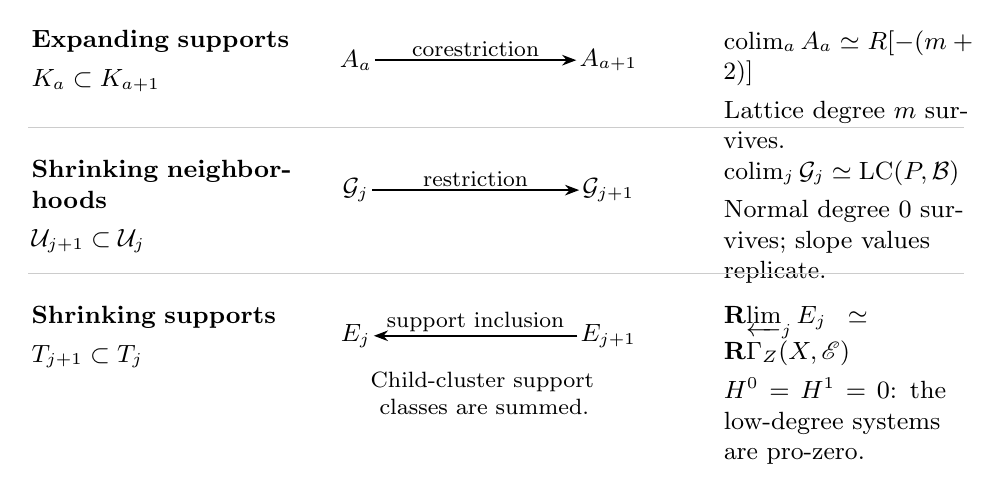
\begin{tikzpicture}[
  x=.98\linewidth,y=1cm,
  every node/.style={font=\small,inner sep=1pt},
  heading/.style={anchor=north west,align=left,text width=.28\linewidth},
  outcome/.style={anchor=north west,align=left,text width=.26\linewidth},
  transition/.style={-{Stealth[length=1.8mm]},semithick}
]
\node[heading] at (0,0)
  {\textbf{Expanding supports}\\[3pt]
   $K_a\subset K_{a+1}$};
\node (a0) at (.35,-.42) {$A_a$};
\node (a1) at (.62,-.42) {$A_{a+1}$};
\draw[transition] (a0) -- node[above,font=\footnotesize]
  {corestriction} (a1);
\node[outcome] at (.74,0)
  {$\colim_a A_a\simeq R[-(m+2)]$\\[3pt]
   Lattice degree $m$ survives.};
\draw[black!20] (0,-1.28) -- (1,-1.28);

\node[heading] at (0,-1.65)
  {\textbf{Shrinking neighborhoods}\\[3pt]
   $\mathcal U_{j+1}\subset\mathcal U_j$};
\node (g0) at (.35,-2.07) {$\mathcal G_j$};
\node (g1) at (.62,-2.07) {$\mathcal G_{j+1}$};
\draw[transition] (g0) -- node[above,font=\footnotesize]
  {restriction} (g1);
\node[outcome] at (.74,-1.65)
  {$\colim_j\mathcal G_j\simeq\operatorname{LC}(P,\mathcal B)$\\[3pt]
   Normal degree $0$ survives; slope values replicate.};
\draw[black!20] (0,-3.13) -- (1,-3.13);

\node[heading] at (0,-3.5)
  {\textbf{Shrinking supports}\\[3pt]
   $T_{j+1}\subset T_j$};
\node (e0) at (.35,-3.92) {$E_j$};
\node (e1) at (.62,-3.92) {$E_{j+1}$};
\draw[transition] (e1) -- node[above,font=\footnotesize]
  {support inclusion} (e0);
\node[outcome] at (.74,-3.5)
  {$\Rlim_j E_j\simeq\RGamma_Z(X,\mathscr E)$\\[3pt]
   $H^0=H^1=0$: the low-degree systems are pro-zero.};
\node[align=center,font=\footnotesize,text width=.40\linewidth]
  at (.485,-4.65) {Child-cluster support classes are summed.};
\end{tikzpicture}
\caption{The three limit directions of
\cref{rem:ind-limit-directions}.  For retained coefficients $R$,
$A_a=\RGamma(L_a,R)[-2]$ is the lattice comparison model, with
$L_{a+1}=p^{-1}L_a$.  On a slope patch $P$, the complex
$\mathcal G_j$ uses neighborhood sections with compact support
along the stratum; its base complex
$\mathcal B=\RGamma_c(Y_t,\mathscr E)$ is retained.  The complex
$E_j$ is instead the support fiber on a fixed ambient bound $X$,
with $Z=\bigcap_jT_j$.}
\label{fig:support-directions}
\end{figure}


\FloatBarrier
\clearpage
\part{Cartier transfers and Laurent supports}\label{part:cartier}
\section{Natural root diagrams and Cartier transfers}
\label{sec:transfers}

The invariant-function calculation makes the source comparison unit
below constant and lets us normalize a single Cartier transfer on a
finite marked algebra. Compact-support finiteness enters the Laurent
argument in \Cref{sec:laurent}. The construction must work on entire finite
diagrams, and its pole bound must survive every iterate: these are the
two inputs the later pro-transfer argument will need.

Fix an exact-height stratum with $1\leq m<n$ and put $r=n-m$.
Throughout this section $G=P_n$ is unchanged.  A sufficiently deep product
subgroup $U\subset P_m\times\GL_r(\Zp)$ will be chosen in the course of the
construction.  Write
\[
 A=\kk[[x,y_1,\ldots,y_{r-1}]],\qquad B=A[1/x],\qquad
 R=B_U=eB',\qquad B'=A'[1/x]
\]
as in \Cref{prop:mark-whole-model}.  In particular, $A'$ is the whole finite
free $A$-algebra with its fixed integral basis, $B'/B$ is finite \'{e}tale,
and $e$ is a $G$-invariant idempotent.  No specialization of $e$ across
$x=0$ will be used.

\subsection{The distribution algebra and the root functor}

Let $B_\infty=\colim_U B_U$ denote the algebra with both full markings.
The compatible lifts of the marked \'{e}tale generators form a torsor
$\mathscr P$ under the affine group scheme
\[
 T=\varprojlim_{[p]}\Gamma_m[p^j]^r.
\]
These are affine torsors, understood through their finite faithfully flat
quotients.  By \Cref{prop:mark-roots},
\begin{equation}
 \cO(\mathscr P)=\colim_j B_\infty^{1/p^{mj}}
                 =B_\infty^{\mathrm{perf}},
 \qquad
 \mathscr P/[p^\ell]T=\Spec B_\infty^{1/p^{m\ell}}.
 \label{eq:trans-full-torsor}
\end{equation}
The $G$-action commutes with $T$; changes of markings act on this identity
and on $T$ by the indicated constant Honda automorphisms.

Here and below a root of a module has a specific meaning.  If $h$ is a
power of $p$ fixing $\kk$ and $M$ is an $R$-module, $M^{1/h}$ is the copy of
$M$ transported along the isomorphism
\[
 R\longrightarrow R^{1/h},\qquad b\longmapsto b^{1/h}.
\]
It is then regarded as an $R$-module by the \emph{inclusion}
$R\subset R^{1/h}$.  Thus a finite locally free $M$ of rank $v$ gives an
$R$-module $M^{1/h}$ of rank $h^rv$.  The map $M^{1/h}\to M$ denoted by
$w\mapsto w^h$ is the transport isomorphism; it is semilinear with respect
to $R^{1/h}\to R$, $b\mapsto b^h$.  This convention applies to maps and
complexes, and does not mean pullback along $R\subset R^{1/h}$ followed
by retaining its rank over the larger ring.

For the remainder of this subsection assume $m>1$. The height-one
case is treated separately in the transfer construction below.
The continuous distribution algebra is
\begin{equation}
 \Lambda=\cO(T)^\vee\simeq\kk[[D_1,\ldots,D_d]],
 \qquad d=(m-1)r.
 \label{eq:trans-distributions}
\end{equation}
Here the dual is the inverse limit of the duals of the finite Hopf
algebras.  We recall why both the dimension and the powers in this
description have these values.  Cartier duality identifies this inverse
limit with the coordinate algebra of the formal group
$(\Gamma_m^D)^r$.  The standard facts used here are the equivalence
between connected $p$-divisible groups and formal Lie groups for which
$[p]$ is finite faithfully flat
over a complete local Noetherian base of residue characteristic $p$,
and finite-flat Cartier duality, which interchanges Frobenius and
Verschiebung; see \citet[\S1.2 and \S\S2.2--2.3, Propositions~1 and~3]{tate1967}.
Our base is the perfect field $\kk$.  On the one-dimensional Honda
group, $F^m=[p]$ and $FV=[p]$.  Duality gives $V^m=[p]$ on the dual;
there $F^m[p]=[p]^m$, and cancellation of the faithfully flat isogeny
$[p]$ gives
\begin{equation}
 F^m=[p]^{m-1}\quad\hbox{on }\Gamma_m^D.
 \label{eq:trans-dual-honda}
\end{equation}
All Frobenius twists in this formula use the Honda model over $\Fp$.
The kernel of $F$ on $\Gamma_m$ has order $p$, whereas $\Gamma_m[p]$ has
order $p^m$.  Thus the kernel of $V$ has order $p^{m-1}$, and the dual
Frobenius has that degree.  A smooth formal group of dimension $s$ has
Frobenius degree $p^s$, so $\dim\Gamma_m^D=m-1$.  When $m>1$ the dual has
no \'{e}tale part: on any finite \'{e}tale $p$-power subgroup Frobenius is
invertible, whereas a sufficiently high iterate of the right side of
\cref{eq:trans-dual-honda} is zero.  The connected $p$-divisible group is
therefore formal, giving \cref{eq:trans-distributions}.
These uses of Cartier duality are at finite flat levels before passing
to the limit.

Choose a positive integer $a_0$ divisible enough to fix the finite
constant field, and set, for $a\geq1$,
\begin{equation}
 q_0=p^{ma_0},\quad q=q_0^a,\quad
 \ell=(m-1)a_0a,\quad h=q^{m-1}=p^{m\ell}.
 \label{eq:trans-powers}
\end{equation}
On the dual formal group, \cref{eq:trans-dual-honda} identifies
$[p^\ell]$ with the $q$-power Frobenius.  Its map on coordinates is the
inclusion
\[
 \sigma_q:\Lambda\longrightarrow\Lambda,
 \qquad D_i\longmapsto D_i^q.
\]
Write $\Lambda^{(q)}=\sigma_q(\Lambda)$ and
\[
 \Lambda_q=\Lambda/(D_1^q,\ldots,D_d^q),\qquad
 \mathsf N_q=\Hom_\kk(\Lambda_q,\kk).
\]
The quotient $T/[p^\ell]T$ has coordinate representation $\mathsf N_q$.
In particular
\[
 \dim_\kk\mathsf N_q=q^d=h^r=p^{m\ell r},
\]
in agreement with the rank of the finite lift torsor.

For a finite-length $\Lambda$-module $E$, regard $E$ as a
$\Lambda^{(q)}$-module through $\sigma_q^{-1}$ and define
\[
 \Coind_q(E)=\Hom_{\Lambda^{(q)}}(\Lambda,E),
 \qquad (a\cdot f)(b)=f(ab).
\]
This is an exact functor, because $\Lambda$ is free over
$\Lambda^{(q)}$ on the monomials $D^\alpha$, $0\leq\alpha_i<q$.
For $E=\kk$ it gives $\mathsf N_q$.  We use the natural change-of-markings
action on coinduction.  Explicitly, if $u$ acts compatibly on $E$, its
action is $(u f)(b)=u(f(u^{-1}b))$.  The inclusion $\sigma_q$ commutes
with this action: its coefficients lie in the finite field fixed by $q$.

Denote by $V_E$ the associated coefficient bundle, obtained by descent
of $\mathscr P\times E$ through translations and then through $U$.
Thus $V_\kk=R$.  A fixed finite diagram of such representations and maps
descends to finite locally free bundles at some finite marking stage.
A plain finite $\Lambda$-module diagram can be given trivial auxiliary
action after shrinking $U$: it factors through a finite-dimensional
quotient of $\Lambda$, whose marking action has finite image.
Coinduced diagrams of arbitrarily large size retain their natural
auxiliary actions; no single $U$ is asserted to act trivially on all of
them.

\begin{proposition}[Natural roots of finite diagrams]
\label[proposition]{prop:trans-roots}
Assume $m>1$. With the powers in \cref{eq:trans-powers}, there is a natural
$G$-equivariant isomorphism
\begin{equation}
 V_{\Coind_q(E)}\simeq (V_E)^{1/h}.
 \label{eq:trans-root-functor}
\end{equation}
It is compatible with the natural auxiliary actions and with every
arrow of a finite diagram.  It preserves exact diagrams and is
compatible with successive coinduction and successive roots.  For any
fixed initial diagram, these assertions hold at every sufficiently
deep finite marking stage, retaining the natural auxiliary action on
each of its coinductions.
\end{proposition}

\begin{proof}
The perfectness in \cref{eq:trans-full-torsor} makes the $h$-power map
an isomorphism on the \emph{total lift torsor}.  Write
$\rho:\cO(\mathscr P)\to\cO(\mathscr P)\otimes_\kk\cO(T)$ for its
coaction.  Absolute powering satisfies
\begin{equation}
 \rho(f^h)=\rho(f)^h
     =(\Fr_h^*\otimes[p^\ell]^*)\rho(f),
 \qquad f\in\cO(\mathscr P).
 \label{eq:trans-power-coaction}
\end{equation}
Here $\Fr_h^*$ raises \emph{all} coefficients, including the base
parameters, to the $h$th power.  Thus this is a map over the matching
Frobenius base, not an endomorphism over the original marked base.
The Honda relation identifies the translation Frobenius with
$[p^\ell]$.  In torsor-action notation the same identity is
$\Fr_h(t\cdot z)=[p^\ell]t\cdot\Fr_h(z)$.
This endomorphism of $T$ gives an isomorphism
\[
 T\xrightarrow{\sim}[p^\ell]T
\]
onto a subgroup of $T$.  It is not an automorphism onto all of $T$.
For example the projection of $[p^\ell]T$ to the level-$\ell$ quotient
is zero.  The group $T$ need not be reduced, although the total torsor
in \cref{eq:trans-full-torsor} is perfect.

It follows from \cref{eq:trans-power-coaction} that, over
$B_\infty^{1/h}$, the same total lift space with structure group
$[p^\ell]T$ is the root of the original $T$-torsor.  Associated-bundle
induction in stages now gives
\[
 V_{\Coind_{[p^\ell]T}^{T}(E)}
   =\pi_*\bigl(V_E\text{ on }\mathscr P/[p^\ell]T\bigr)
   \simeq (V_E)^{1/h},
\]
where $\pi:\Spec B_\infty^{1/h}\to\Spec B_\infty$ is the finite root
map.  The pushforward is the restriction of scalars specified above.
One can verify the equality without a choice of a torsor point:
after a faithfully flat trivialization it is the usual evaluation
isomorphism for coinduced equivariant functions, and that isomorphism
commutes with the two projections in the descent diagram.  It therefore
descends, is natural in $E$, and identifies each morphism of any finite
diagram.  This also proves exactness, since the trivialized functors
are exact and the base changes are faithfully flat.

All the maps used here commute with $G$.  They also commute with the
changes of markings, since $[p^\ell]$ is central and the chosen power
fixes $\kk$.  For two powers, the identities
$(z^{h_1})^{h_2}=z^{h_1h_2}$ and
$[p^{\ell_2}][p^{\ell_1}]=[p^{\ell_1+\ell_2}]$ show that the two
resulting torsor maps are equal.  The evaluation map for coinduction
in stages has the same composition law.  This proves the asserted
coherence, including the maps of the diagrams, rather than only an
identification of their terms.

Finally, the original finite diagram, its torsor quotient, and its
coaction involve finitely many matrix coefficients and relations.
They descend through the filtered union of finite \'{e}tale marking
algebras.  Choose one stage containing this data and shrink $U$ so that
the original diagram has the required auxiliary action there.  At
every coinduction level the preceding identity is still the same
intrinsic power identity, with its natural auxiliary action; it
therefore descends to that stage.  Equivariance can be checked after
the one faithfully flat full-marking extension, since $G$ preserves
each finite marking algebra.  This does not require intersecting
depth conditions for individual elements of $G$, or making all high
coinduced representations trivial under $U$.
\end{proof}

The elementary pairing underlying coinduction will also be useful.
Let $\kappa_q:\Lambda\to\Lambda^{(q)}$ extract the coefficient of
$\prod_iD_i^{q-1}$ in the displayed free basis.  The pairing
$(a,b)\mapsto\kappa_q(ab)$ is perfect: modulo the maximal ideal of
$\Lambda^{(q)}$ its matrix pairs $D^\alpha$ with
$D^{(q-1)\mathbf1-\alpha}$, and hence is invertible; its determinant
is a unit already over $\Lambda^{(q)}$.  Thus coinduction is naturally
isomorphic to scalar extension as a functor of plain modules, once
this functional is fixed.  This last choice need not identify the
auxiliary actions, so the action supplied by
\Cref{prop:trans-roots} will always be retained.

\subsection{A volume at one finite marking stage}

Use continuous differentials on the formal parameter ring and their
localizations and finite \'{e}tale base changes; write this module as
$\widehat\Omega^1_{R/\kk}$.  It is free of rank $r$ before any perfection.

For a finite translation quotient $H$, a \emph{translation augmentation}
means a nonzero $H$-equivariant map $\lambda:\cO(H)\to\kk$, with trivial
action on $\kk$. Equivalently, it is an invariant integral:
$(\id\otimes\lambda)\Delta(a)=\lambda(a)1$.
For $m>1$ and the quotient indexed by $q$, this is a $\Lambda$-linear
map $\mathsf N_q\to\kk$. The term refers to this invariant functional,
not to the Hopf counit.

\begin{proposition}[Invariant volume and scalar comparison]
\label[proposition]{prop:trans-volume}
After one finite marking shrink to a pro-$p$ subgroup,
$\widehat\Omega^1_{R/\kk}$ has a
$G$-invariant frame.  In particular it has a $G$-invariant volume
generator $\eta\in\widehat\Omega^r_{R/\kk}$.

For a finite root order $h$ fixing $\kk$, the normalized Cartier
functional
\begin{equation}
 T_{\eta,h}:R^{1/h}\longrightarrow R,
 \qquad T_{\eta,h}(z)=\frac{\Cartier^{\log_p h}(z^h\eta)}{\eta}
 \label{eq:trans-cartier-functional}
\end{equation}
is $R$-linear and generates $\Hom_R(R^{1/h},R)$ as a module over
$R^{1/h}$.  A nonzero translation augmentation at the corresponding
finite torsor level induces a scalar multiple of this functional;
the scalar belongs to the chosen finite constant field.
\end{proposition}

\begin{proof}
The intermediate order-$p$ root cover is a torsor under the height-one
Frobenius quotient of translations, of rank $p^r$.  Over the chosen
Honda constants this quotient is $\alpha_p^r$ for $m>1$ and $\mu_p^r$
for $m=1$.  This follows by taking the first Frobenius kernel of the
Honda group; its Verschiebung is zero in the first case and invertible
in the second.  These finite Hopf algebras and their Lie spaces are
defined over a finite field.  Their continuous marking actions factor
through a finite group.  Shrink $U$ to fix the quotient and a Lie basis.
For $m=1$ choose the standard toral basis of the fixed $\mu_p^r$.
Finite presentation of the coaction descends its torsor action to a
finite stage.  Torsor freeness identifies the resulting invariant
vector fields with a basis
\[
 \delta_1,\ldots,\delta_r
 \quad\hbox{of }\operatorname{Der}_R(R^{1/p},R^{1/p}).
\]
For completeness this freeness can be checked after trivializing the
torsor: the vectors are $\partial/\partial z_i$ on $\alpha_p^r$ and
$z_i\partial/\partial z_i$ on $\mu_p^r$.  Their coefficient matrices
are invertible, and invertibility descends faithfully flatly.

For $b\in R$, define
\begin{equation}
 \partial_i(b)=\bigl(\delta_i(b^{1/p})\bigr)^p.
 \label{eq:trans-frame}
\end{equation}
This formula is additive, satisfies the ordinary Leibniz rule, and is
$\kk$-linear because $\kk$ is perfect.  To see that it is a frame, let
$(t_1,\ldots,t_r)=(x,y_1,\ldots,y_{r-1})$, a $p$-basis after the
finite \'{e}tale base change.  Write
\[
 \delta_i=\sum_j a_{ij}\frac{\partial}{\partial t_j^{1/p}}.
\]
Then $\partial_i=\sum_j a_{ij}^p\partial/\partial t_j$ and the new
determinant is $\det(a_{ij})^p\in R^\times$.  The derivations commute
with $G$, because the full-marking action commutes with translations
and with powers.  The identities descend to this same finite stage:
they hold after the faithful full-marking extension, and $G$ preserves
$R$.  The dual frame and its top wedge give $\eta$.  All differentials
in this construction were taken at a finite root stage.

We describe the Cartier operator used in
\cref{eq:trans-cartier-functional}.  If
$dt=dt_1\wedge\cdots\wedge dt_r$ and $h=p^\nu$, the unique $p$-basis
expansion of a form is
\[
 f\,dt=\sum_{0\leq\alpha_i<h} f_\alpha^h t^\alpha\,dt,
 \qquad f_\alpha\in R.
\]
The operator is
\begin{equation}
 \Cartier^\nu(f\,dt)=f_{(h-1)\mathbf1}\,dt.
 \label{eq:trans-cartier-coordinates}
\end{equation}
For power series the expansion groups the exponents modulo $h$;
localization and finite \'{e}tale base change preserve it.  First take
$h=p$.  In one variable the de Rham differential on a residue exponent
other than $p-1$ gives an exact term, while the last exponent gives the
class of $t^{p-1}dt$.  Tensoring these one-variable complexes proves
the Cartier isomorphism in $r$ variables, and iterating it gives
\cref{eq:trans-cartier-coordinates} for $h=p^\nu$.  The inverse of the
one-step isomorphism is
characterized on one-forms by $db\mapsto[b^{p-1}db]$ and by
multiplication on exterior powers.  This characterization shows that
the formula commutes with coordinate changes and \'{e}tale base change.
For the customary inverse-Frobenius convention and its duality
interpretation, see \citet[Definition~2.1 and Example~2.23]{blickleBockle2011}.
It is continuous on the indicated formal coefficient modules.  In
particular it commutes with $G$ and satisfies
$\Cartier^\nu(b^h\omega)=b\Cartier^\nu(\omega)$.

\Cref{eq:trans-cartier-coordinates} proves the asserted
linearity and dual-generator property.  More explicitly, for
$\eta=dt$ the pairing
\[
 (u,v)\longmapsto T_{dt,h}(uv)
\]
on $R^{1/h}$ pairs the $R$-basis $t^{\alpha/h}$ with its
complementary basis $t^{((h-1)\mathbf1-\alpha)/h}$, and has invertible
matrix.  Replacing $dt$ by a volume generator multiplies by units on
the source and target and preserves perfectness.  This establishes
the claim without applying a finite-type smoothness theorem to the
completed power-series ring.

The torsor augmentation has the same dual-generator property.  Here
is a finite-level verification.  The coordinate algebra of the
translation quotient is a tensor product of truncated polynomial
algebras $\kk[z_i]/(z_i^h)$, with its Honda Hopf structure.  A nonzero
translation-invariant functional $\lambda$ gives a pairing
$\lambda(ab)$.  Its radical is a translation-stable ideal: invariance
of $\lambda$ and the antipode identity show that the map to the dual
regular representation is equivariant.  If the radical is proper,
it is contained in the augmentation ideal, since this coordinate
algebra is local.  For a translation-stable ideal $I$ contained there,
apply $\id\otimes\epsilon$ to $\Delta(I)\subset\cO(H)\otimes I$;
the counit identity gives $I=0$.  The radical cannot be the whole
algebra because $\lambda\ne0$.  The pairing is therefore perfect.
After a faithfully flat trivialization this is precisely the pairing
of the torsor functional, so its perfectness descends.

There is a useful precision about the comparison.  The dual module is
rank one over the \emph{source} $R^{1/h}$.  Thus the two functionals
initially differ by
\begin{equation}
 \tau(z)=T_{\eta,h}(u z),\qquad u\in(R^{1/h})^\times,
 \label{eq:trans-source-unit}
\end{equation}
not by an a priori constant multiplying the output.  Both maps are
$G$-equivariant, and the generator property makes $u$ unique, hence
$G$-invariant.  By \Cref{thm:tower-comparison,cor:ind-functions}, its
image after perfected geometric extension and full markings is a
constant on $(\mathcal N_m^r)_{\mathrm{ind}}$.  This extension is
injective on the finite algebraic root ring: power-series expansion
on the analytic annuli is injective in each entry of the whole finite
free basis, remains so after the idempotent summand, and full marking
is faithfully flat.  The coefficient-only
$|\kk|$-Frobenius fixes its finite model, and therefore fixes this
constant.  Consequently $u\in\kk^\times$, with the understood finite
enlargement if the model was defined there.  Since $h$ fixes $\kk$,
\cref{eq:trans-source-unit} is the required scalar comparison.
\end{proof}

\subsection{One transfer, all iterates, and whole-model pole bounds}

When $m>1$ put $h_0=q_0^{m-1}$ as in
\cref{eq:trans-powers}; when $m=1$ choose a power $h_0=p^{\nu_0}>1$
fixing the same finite constants.  In either case set
$\nu_0=\log_p h_0$.

\begin{proposition}[The fixed normalized transfer]
\label[proposition]{prop:trans-cartier}
At the finite marking stage of \Cref{prop:trans-volume}, the operator
\begin{equation}
 S(f)=\frac{\Cartier^{\nu_0}(f\eta)}{\eta}\quad(f\in R)
 \label{eq:trans-S}
\end{equation}
is continuous, $\kk$-linear, and $G$-equivariant.  It satisfies
$S(b^{h_0}f)=bS(f)$.  For $m>1$, the maps on $R$ induced by nonzero
translation augmentations $\mathsf N_{q_0^a}\to\kk$, after the root
identification, are nonzero scalar multiples of $S^a$.  For $m=1$ one
can choose the toral frame so that
\begin{equation}
 S\Fr^{\nu_0}=1.
 \label{eq:trans-height-one-split}
\end{equation}

Extend $S$ to $B'$ by $S(f)=S(ef)$, with image in $eB'$.  There is a
fixed integer $c\geq0$ such that, for every integer $D$,
\begin{equation}
 S(x^{-D}A')\subset x^{-\lceil D/h_0\rceil-c}A'.
 \label{eq:trans-pole-bound}
\end{equation}
Every sufficiently large $D_0$ makes
$\mathcal P=x^{-D_0}A'$ stable under $S$.  Every fixed bounded-pole
lattice, including any compact family of cochains with values in it,
is carried into $\mathcal P$ by all sufficiently large iterates.

The volume, its inverse, the whole trace-pairing matrices and their
inverses have one fixed pole bound $c'$.  In the normalized basis
$b_i^{1/h}$, $h=h_0^a$, their transported matrices have pole losses at
most $c'/h$.  The normalized Cartier maps are adjoint to the inclusions
of root Laurent representatives under the residue pairings with the
transported volumes.
\end{proposition}

\begin{proof}
The formula and \Cref{prop:trans-volume} give equivariance and
$h_0^{-1}$-linearity.  This is $\kk$-linearity because $h_0$ fixes the
finite field.  Continuity follows by grouping finitely many residue
exponents in the $h_0$-basis expansion; multiplication by the fixed
volume and its inverse is continuous on bounded-pole steps.
The intermediate volume factors cancel under composition, so
$S^a(f)=\Cartier^{a\nu_0}(f\eta)/\eta$ for every $a\geq1$.

Suppose first that $m>1$.  Put
$s_q=\prod_iD_i^{q-1}\in\Lambda_q$.  A $\Lambda$-linear functional
$\mathsf N_q\to\kk$ is evaluation at a socle element of $\Lambda_q$.
Its space is the one-dimensional line generated by evaluation at
$s_q$.  Make $U$ pro-$p$.  The action on this line is a continuous
character to $\kk^\times$, a group of order prime to $p$, so it is
trivial.  The maps therefore descend with their natural actions.
Successive coinduction composes the basic socle evaluations into
evaluation at
\[
 \prod_{j=0}^{a-1}s_{q_0}(D_1^{q_0^j},\ldots,D_d^{q_0^j})
       =\prod_iD_i^{q_0^a-1},
\]
which is nonzero in $\Lambda_{q_0^a}$.  Thus these composites do not
vanish.  The coherence of \Cref{prop:trans-roots} identifies their
coefficient maps with the root-twisted composites of
$T_{\eta,h_0}$.  In selfmap notation these are $S^a$.
\Cref{prop:trans-volume} identifies any other nonzero augmentation
with a nonzero constant multiple; the constants introduce no
semilinear twist because all chosen powers fix $\kk$.

Suppose now that $m=1$. We use the order-$p$ torsor
$C=R^{1/p}$ under the fixed group $\mu_p^r$ from
\Cref{prop:trans-volume}. Its character decomposition is strongly
graded by $(\Z/p\Z)^r$, with neutral component $R$ and invertible
character components
\citep[Theorem~12.12 and Remark~12.13]{milne2017}.
The strong grading uses the torsor hypothesis: after a faithfully
flat trivialization, each character component is free of rank one
and multiplication between components is an isomorphism. These
properties descend to $R$.
Zariski locally on $\Spec R$, choose generators $z_i$ of the
fundamental character components. Strong grading makes each $z_i$
a unit, with $b_i=z_i^p\in R^\times$. The monomials $z^\alpha$,
$0\leq\alpha_i<p$, form an $R$-basis of $C$. Taking $p$th powers
shows that the $b^\alpha$ form an $R^p$-basis of $R$, so the $b_i$
are a $p$-basis.

For the standard toral Lie basis,
$\delta_i(z_j)=\delta_{ij}z_j$. \Cref{eq:trans-frame} gives
$\partial_i(b_j)=\delta_{ij}b_j$, so the already constructed volume
is locally
\[
 \eta=d\log b_1\wedge\cdots\wedge d\log b_r.
\]
On overlaps a different choice has $z_i'=c_i z_i$ with
$c_i\in R^\times$, hence $b_i'=c_i^p b_i$ and
$d\log b_i'=d\log b_i$. These local descriptions therefore agree
with the global volume. We retain this standard toral normalization;
the comparison constants multiply the torsor functionals.
The logarithmic Cartier formula gives $\Cartier(\eta)=\eta$.
Consequently, for every chosen $h_0=p^{\nu_0}$ fixing $\kk$,
\[
 S(f^{h_0})
   =\frac{\Cartier^{\nu_0}(f^{h_0}\eta)}{\eta}
   =f\,\frac{\Cartier^{\nu_0}(\eta)}{\eta}
   =f.
\]
This proves \cref{eq:trans-height-one-split} at the existing finite
frame stage. The natural auxiliary actions at higher levels are
retained; no splitting of a higher torsion quotient or further
shrink of $U$ is required. No positive-dimensional local distribution
ring is used in this case.

We next prove the pole bound in the whole model.  Fix an $A$-basis
$b_1,\ldots,b_v$ of $A'$.  The finite \'{e}tale base change makes
$B'^{1/h_0}$ free over $B$ on
\[
 b_i^{1/h_0}x^{\alpha_1/h_0}
     y_1^{\alpha_2/h_0}\cdots y_{r-1}^{\alpha_r/h_0},
 \qquad 0\leq\alpha_j<h_0.
\]
The $B$-linear map $T_{\eta,h_0}$ after multiplication by $e$, with
output included in $B'$, is a fixed finite matrix in these bases.
Its entries belong to $B$ and so have a common finite $x$-pole bound.
For $f\in x^{-D}A'$, its root is a sum of
$x^{-D/h_0}a_i^{1/h_0}b_i^{1/h_0}$, with $a_i\in A$.
Group the exponents in each $a_i^{1/h_0}$ modulo the integral lattice.
The resulting coefficients lie in $A$.  Reducing $-D$ modulo $h_0$
loses at most $\lceil D/h_0\rceil$ integral powers of $x$.
The fixed matrix contributes at most a further $c$, proving
\cref{eq:trans-pole-bound} for all $D$, including negative $D$.
This also proves continuity on compact coefficient lattices.

If $D_{a+1}\leq D_a/h_0+c+1$, then
\[
 D_a\leq h_0^{-a}D+(c+1)\frac{1-h_0^{-a}}{1-h_0^{-1}}.
\]
Choose $D_0>(c+1)/(1-h_0^{-1})$.  The same inequality implies
$\lceil D_0/h_0\rceil+c\leq D_0$ and, for each fixed $D$, eventually
$D_a\leq D_0$.  The estimates apply to the whole lattice, uniformly
over any compact parameter set.  A compact bounded-pole cochain
family uses one such $D$, so the assertion about cochains follows as
well.

For the trace and volume assertion, set
\[
 \theta=d\log x\wedge dy_1\wedge\cdots\wedge dy_{r-1}.
\]
Write $\eta=a_R\theta$ with $a_R\in R^\times$.  Extend its coefficient
to the unit $a=a_R+(1-e)\in B'^\times$ and use $a\theta$ on the whole
algebra.  The trace form of the finite \'{e}tale algebra is perfect;
therefore the matrices
\[
 \bigl(\Tr_{B'/B}(b_i b_j)\bigr)_{ij},\qquad
 \bigl(\Tr_{B'/B}(a b_i b_j)\bigr)_{ij}
\]
and their inverses have entries in $B$.  The multiplication matrices
of $e,a,a^{-1}$ do also.  Taking a maximum bounds all their poles by
one $c'$.  Transport by the root isomorphism replaces every matrix
entry by its $h$th root.  Its pole bound in the original $x$-valuation
is consequently $c'/h$.  The volume at this level is
\[
 \eta_h=a^{1/h}\,d\log x^{1/h}\wedge
                   dy_1^{1/h}\wedge\cdots\wedge dy_{r-1}^{1/h}.
\]
This is transport along an isomorphism, not differential pullback
under an inseparable map.

Finally take a finite Laurent principal-part representative $w$ on
one root grid and a bounded-pole coefficient on the next grid, and
pair them by the coefficient residue of their product times
$\eta_h$, after the finite \'{e}tale trace.  In the logarithmic
$x$-coordinate the residue selects exponent zero; in each ordinary
$y$-coordinate it selects exponent $-1$.  \Cref{eq:trans-cartier-coordinates} therefore gives
\begin{equation}
 \langle w,T_{h,hh_0}(f)\rangle_h
       =\langle \iota w,f\rangle_{hh_0},
 \label{eq:trans-residue-adjoint}
\end{equation}
where $T_{h,hh_0}$ is the $h$-root of $T_{\eta,h_0}$ and $\iota$ is
inclusion of the same Laurent expression on the finer grid.
For instance the ordinary one-variable test is
$h_0i+j=-1$ on both sides; the logarithmic test is $h_0i+j=0$.
The coefficient field is fixed by $h_0$, so taking the selected
coefficient introduces no field twist.  Finite \'{e}tale trace
commutes with this calculation, since its root matrix is the
transported trace matrix.  Multiplication by the volume coefficient
and its inverse cancels as in
\cref{eq:trans-cartier-functional}.  Thus the scalar monomial check
proves \cref{eq:trans-residue-adjoint} in the whole basis and then
after $e$.  Continuity extends the identity whenever a convergent
Laurent expression defines a residue functional.  This is the
adjoint identity used below; no trace for the purely inseparable
root extension is involved.
\end{proof}

\begin{lemma}[One bound for a fixed finite diagram]
\label{lem:trans-diagram-bound}
Fix a finite Yoneda diagram of translation representations, descend
it at a finite marking stage, and fix a cohomological degree.  Its
successive boundary maps can be represented by an operator on
cocycles that loses at most one fixed $x$-pole order.  Under
\Cref{prop:trans-roots}, all of its coinduced diagrams use the roots
of this same operator and its chosen splittings.
\end{lemma}

\begin{proof}
Every term and image bundle is finite locally free on the affine
scheme $\Spec R$.  Each surjection onto such an image has an
underlying $R$-linear section.  Choose these finitely many sections
once.  Embed their finite projective modules in finite free modules
and choose finitely generated whole $A$-lattices; each section is
then a finite matrix over the localization and has a fixed pole
loss.  The group action on a fixed lattice has a uniform pole bound,
by the finite torsor realization and the bounded-step continuity of
\Cref{lem:cts-exact,prop:mark-whole-model}.  Since $g(x)/x$ is an
integral unit, the same bound applies to every shift of that lattice.
The finitely many group differentials and chosen sections computing
the composite boundary thus have a common total pole loss.  This
constructs the required operator on continuous cocycles, with their
bounded-pole convention.

The natural identity \cref{eq:trans-root-functor} carries the entire
diagram, including its arrows, to its root diagram.  Transport each
of the already chosen sections by the same root isomorphism.
Computing the boundary with those sections is exactly the root of
the original computation.  Hence the increasing ranks of the
coinduced representations require no new choices of matrices or
new pole estimate.  This statement concerns realization of a fixed
diagram; comparisons of extension classes after one common
auxiliary shrink are supplied in \Cref{sec:pro-transfer}.
\end{proof}

\section{The Laurent model for analytic compact supports}
\label{sec:laurent}

We now express the compact supports of the geometric calculation as
convergent Laurent series. The output is an explicit module with the
actual stabilizer action and finite cohomology and homology. Its
finite-field form will carry the residue map that is transpose to the
Cartier transfer, including series with unbounded root denominators.

Fix $1\leq m<n$, put $r=n-m$ and $s=r-1$, and retain the
whole finite free model
\[
 A=\kk[[x,y_1,\ldots,y_s]],\qquad B=A[1/x],\qquad
 A'=\bigoplus_{\nu=1}^{N}A b_\nu,\qquad B_U=eA'[1/x]
\]
of \cref{prop:mark-whole-model}.  Thus $A'[1/x]$ is finite
\'{e}tale over $B$, its multiplication laws in the displayed basis are
integral, and $e$ is a $G$-invariant idempotent.  All operations involving
$e$ below take place in the whole free module.  In particular no
specialization of $e$ at $x=0$ is used.

Write $F=\Cflat$, fix its absolute value, and let $X$ be the perfected
characteristic-$p$ analytic domain
\[
 0<|x|<1,\qquad |y_j|<1\quad(1\leq j\leq s)
\]
over $F$.  Its finite marked cover is denoted by $Z_U$.  The sheaf
$\cO^\flat$ on this characteristic-$p$ space is its structural sheaf.
The present calculation consequently concerns a different space from the
untilted affine line in \cref{prop:kum-line}.

\subsection{Complete Laurent steps}

For a compact profinite set $\mathcal D$, put
$R_{\mathcal D}=C(\mathcal D,F)$, with its supremum norm.  An empty
parameter set will not be used; when there is no parameter we take a
one-point set.  Set
\[
 \mathcal E=\Z[1/p]\times\bigl(\Z[1/p]_{>0}\bigr)^s,
 \qquad |J|=J_1+\cdots+J_s.
\]
If $s=0$, the second factor has one element and $|J|=0$.
For $L>\delta>0$ define
\begin{equation}\label{eq:laurent-weight}
 w_{L,\delta}(I,J)=
 \begin{cases}
 LI-\delta|J|,&I\geq0,\\
 \delta I-\delta|J|,&I<0.
 \end{cases}
\end{equation}
Let $\mathscr L_{L,\delta}(\mathcal D)$ consist of the sums
\[
 f=\sum_{(I,J)\in\mathcal E}a_{I,J}x^Iy^{-J},
 \qquad a_{I,J}\in R_{\mathcal D},
\]
such that the numbers
$\|a_{I,J}\|_{\sup}\exp(-w_{L,\delta}(I,J))$ tend to zero outside
finite subsets of $\mathcal E$.  Equip this space with the maximum of
these numbers as norm.  It is a complete nonarchimedean normed module:
coefficientwise limits of a Cauchy sequence have uniformly small tails,
which proves both the required decay and convergence in the norm.
Finite sums are dense.  Define
\[
 \mathscr L(\mathcal D)=\colim_{L,\delta}
       \mathscr L_{L,\delta}(\mathcal D).
\]
The transitions increase $L$ and decrease $\delta$.  They are norm
nonincreasing, since these changes increase every weight.  Rational pairs
$L>\delta>0$, or the sequence $(L,\delta)=(j,j^{-1})$ with $j\geq2$,
are cofinal.  The colimit here and below has the complete-step convention
of \cref{sec:continuous}; a parameter family belongs to one step.

Multiplication by an element of $B$ is multiplication of Laurent series
followed by discarding every monomial whose exponent in some $y_j$ is
nonnegative.  This prescription is well defined in the complete steps.
Indeed, if $a\in x^{-c}A$, every monomial of $a$ has exponents
$(A_0,B_0)$ with $A_0\geq-c$ and all $(B_0)_j\geq0$.  Whenever its
product survives the projection,
\begin{equation}\label{eq:laurent-matrix-bound}
 w_{L,\delta}(I+A_0,J-B_0)
       \geq w_{L,\delta}(I,J)-Lc.
\end{equation}
This follows because the increasing piecewise linear function
$I\mapsto LI$ for $I\geq0$, $I\mapsto\delta I$ for $I<0$, has slopes
between $\delta$ and $L$.  At a fixed root grid, multiplying one
monomial by $a$ gives a convergent series: after projection only finitely
many $y$-exponents survive below the original pole orders, and the
remaining $x$-orders tend to infinity.  The bound extends multiplication
from finite sums to arbitrary sums, proves its continuity, and justifies
associativity by dense finite-sum approximation.  A matrix with entries
in $x^{-c}A$ has the same bound, up to the maximum norm of its finitely
many entries.

Consequently $e$ is a continuous chain-compatible idempotent on the
whole ambient Laurent module.  We use the notation
\[
 \mathscr W_{\mathcal D}
   =e\bigl(\mathscr L(\mathcal D)\otimes_A A'\bigr),
 \qquad
 W_{\mathcal D}
   =e\bigl(\mathscr L(\mathcal D;\kk)\otimes_A A'\bigr),
 \qquad W=W_{\{*\}},
\]
where $\mathscr L(\mathcal D;\kk)$ denotes the same sums with
coefficients in $C(\mathcal D,\kk)$.  The tensor notation means the
finite sum on the displayed basis, with the multiplication action just
defined; it introduces no additional completion.  The image of $e$ in
each step is closed, since it is the kernel of $1-e$, and is therefore
complete.

For finite-field coefficients the decay condition has a useful strong
consequence.  For every real $M$, a family in one step has only finitely
many nonzero coefficients with $I\leq M$, uniformly on $\mathcal D$.
Indeed, every nonzero coefficient has supremum norm one, whereas
\[
 I\leq M\quad\Longrightarrow\quad
 w_{L,\delta}(I,J)\leq L\max(M,0).
\]
Infinitely many such coefficients would contradict decay.  Each of the
remaining finitely many coefficient functions is locally constant.
In particular bounded-$x$ truncation produces a locally constant family
of finite principal parts, even when the original exponents have
unbounded $p$-power denominators.  For a one-point parameter the steps
are separable: their finite sums have coefficients in the finite field
and indices in the countable set $\mathcal E$.  Thus the complete steps
of $W$ are Polish additive groups.  A condition that coefficients vanish
outside a prescribed subset, for example $I\geq a>0$, is closed on each
such step.

\subsection{The support complex and coefficient descent}

Let $Q_k=|\kk|$.  The operator $\varphi$ used in this subsection raises
coefficients in $F$ to their $Q_k$th powers and fixes $x^I$, $y^{-J}$,
and every $b_\nu$.  It fixes the structure constants of $A'$ and the
matrix of $e$, since they are defined over $\kk$.  This is
\emph{coefficient-only} Frobenius.  For a complex $K$ with this operator
write
\[
 K^{\varphi=1}=\operatorname{fib}(\varphi-1:K\longrightarrow K).
\]

\begin{proposition}[Laurent support comparison]\label[proposition]{prop:laurent-model}
With the uniform compact-support convention of
\cref{lem:tower-supports}, there are natural quasi-isomorphisms
\begin{equation}\label{eq:laurent-descent}
 \RGamma_c(Z_U,\cO^\flat;\mathcal D)
       \simeq\mathscr W_{\mathcal D}[-r],
 \qquad
 \RGamma_c(Z_U,\cO^\flat;\mathcal D)^{\varphi=1}
       \simeq W_{\mathcal D}[-r].
\end{equation}
They are compatible with finite marking maps, the idempotent $e$, and
the actions defined over $\kk$.  The support cohomology is therefore
concentrated in cohomological degree $r$, both before and after
coefficient descent.  Every fixed normalized root basis
$b_1^{1/h},\ldots,b_N^{1/h}$ gives the same module and the same
complete-step category.
\end{proposition}

\begin{proof}
We first calculate on $X$ with scalar coefficients.  Compact bounds
are cofinal among boxes
\[
 K(a,b,\rho)=
 \{a\leq|x|\leq b,\ |y_j|\leq\rho\ (1\leq j\leq s)\},
 \qquad 0<a<b<\rho<1.
\]
In fact a quasicompact bound has its $x$-norm bounded away from zero and
all coordinate norms bounded strictly below one; one can then choose
$\rho$ larger than its $x$-bound and every $y$-bound.  Interleaving a
slightly smaller closed box and a slightly larger open box gives the
same support colimit.  This permits strict gaps in every radius used
below and avoids assertions about a particular higher-rank boundary
point.

The complement of a box is the union of the two $x$-exteriors and the
$s$ individual $y$-exteriors.  Its finite \v Cech restriction diagram,
augmented by sections on $X$, calculates the support fiber.
Every intersection is a product of open discs, punctured discs, and
annuli.  Exhaust it by a countable sequence of closed polyannuli and
polydiscs, after adjoining all coordinate roots. The root polydisc,
rational-localization and product constructions make these closed domains
affinoid perfectoid
\citep[Proposition~5.20, Theorem~6.3\textup{(i)--(ii)}, and Proposition~6.18]{scholzePerfectoid2012}.
Their structural sheaf is v-acyclic by
\cite[Proposition~8.8]{scholzeDiamonds2017}.  Their function algebras
are the corresponding completed Laurent algebras.  The restriction
maps have dense image: finite Laurent polynomials belong to both
domains and are dense in the smaller-domain algebra.  With parameters,
finite sums whose coefficients are in $R_{\mathcal D}$ have the same
property.  Equivalently, first approximate a continuous parameter
family by a finite clopen partition and then approximate its finitely
many values by Laurent polynomials.  The complete normed-space
inverse-limit lemma, \cref{lem:kum-banach-limits}, eliminates the first
derived inverse limit.  There are no higher derived limits for a
countable sequence.  Thus these open intersections have their ordinary
Laurent functions in degree zero, with no additional cohomology.

Here is the resulting splitting of the support diagram.  In an
unpunctured coordinate $y_j$, a function on the exterior annulus is the
sum of its nonnegative and strictly negative Laurent parts.  The
nonnegative part extends to the whole disc, since it converges at every
radius less than one.  Its summand in the restriction complex is
contractible.  The negative part is the quotient summand, in degree
one.  These projections have norm at most one on each closed annulus;
on open domains one first inserts a radius gap.  They are
$R_{\mathcal D}$-linear and act coefficientwise in the other
coordinates.

For the punctured coordinate write an exterior pair as
$(f_{\rm in},f_{\rm out})$.  The negative part of $f_{\rm in}$ extends
to the whole punctured disc: convergence towards zero is the only
extra condition for a negative-power series.  Likewise the
nonnegative part of $f_{\rm out}$ extends to the whole punctured disc.
Subtracting these global functions diagonally leaves the unique pair
\[
 \bigl(f_{\rm in,+}-f_{\rm out,+},\,
       f_{\rm out,-}-f_{\rm in,-}\bigr).
\]
Encode it by the single Laurent series
\[
  f=(f_{\rm in,+}-f_{\rm out,+})
       -(f_{\rm out,-}-f_{\rm in,-}).
\]
Thus its normal representative is $(f_+,-f_-)$.  The minus sign
ensures that multiplication or substitution crossing the exponent
$I=0$ is represented by the usual Laurent operation: eliminating an
outer nonnegative part by a diagonal section introduces its negative
at the inner end.  This quotient is again in degree one, and it
retains every exponent $I\in\Z[1/p]$, including zero exactly once.

Apply these splittings successively to the finite product restriction
diagram.  A summand which extends in any one coordinate is
contractible by the corresponding one-coordinate splitting.  The only
remaining summand has every $y$-exponent negative and the indicated
two-ended $x$-representative.  It lies in degree $s+1=r$.
The splittings commute in distinct coordinates, so this is a
calculation of the entire complex, not only of its highest quotient.
It also proves the assertion for $s=0$.

For the surviving inner positive $x$-powers choose a radius
$\exp(-L)$ slightly below the inner support radius.  For the surviving
negative $x$-powers and negative $y$-powers choose a common outer
radius $\exp(-\delta)$ slightly above every outer support radius.
Their Gauss norms are exactly
\[
 \|a_{I,J}\|_{\sup}\exp(-LI+\delta|J|)
 \quad(I\geq0),\qquad
 \|a_{I,J}\|_{\sup}\exp(-\delta I+\delta|J|)
 \quad(I<0).
\]
Convergence on a closed polyannulus is precisely decay outside finite
subsets for these norms.  Every support class has these bounds after
inserting the radius gaps.  Conversely a series in one such step
converges on the smaller inner domain and the larger outer collars,
and hence supplies a class for a box with separated radii.  Enlarging
supports decreases the inner radius and increases the outer radii;
on these representatives the map retains the same coefficients.
The support colimit is therefore exactly $\mathscr L(\mathcal D)$.
This calculation uses the finite restriction diagram followed by a
filtered colimit of supports.  It does not interchange that colimit
with an inverse limit of shrinking supports.

We next pass to the actual finite marked algebra.  On a closed base
chart with perfectoid algebra $R$, the whole algebra
\[
 A'[1/x]\otimes_B R=\bigoplus_{\nu=1}^N Rb_\nu
\]
is already complete as a finite free $R$-module.  It is finite
\'{e}tale and affinoid perfectoid by
\cite[Theorem~6.1(i)]{scholzeDiamonds2017}.  Relative Frobenius for an
\'{e}tale algebra is an isomorphism
\cite[Lemma~41.14.3, Tag~0EBS]{stacks}; consequently this algebra is
also the perfected marked extension, rather than only an
unperfected approximation.  Restrictions use the same whole basis,
so the function complex is the finite sum of the scalar complexes.
The matrix $e$ commutes with every restriction and is an actual chain
idempotent.  Taking its image commutes with the finite fibers and
filtered support colimit.  For the intermediate inverse limits its
image remains complete and the transition maps remain dense: apply
the target idempotent to ambient approximants.  Hence the preceding
inverse-limit argument applies there as well.

This computation uses all compact supports on $Z_U$.  Pullbacks of
quasicompact bounds under a finite map are quasicompact, and the image
of a quasicompact bound is a quasicompact bounded subset of $X$.
Thus pulled-back boxes form a cofinal support system upstairs.  This
establishes the first quasi-isomorphism in
\cref{eq:laurent-descent} on the actual cover.

Coefficient Frobenius and its inverse are continuous between steps.
For example, raising a coefficient to its $Q_k$th power changes a
weight $w$ to $Q_kw$; this is the step with parameters
$(Q_kL,Q_k\delta)$, followed if needed by a cofinal enlargement.
It remains to check surjectivity of $\varphi-1$, including parameters.
For $b\in F$, the equation
\[
 a^{Q_k}-a=b
\]
has a solution with $|a|\leq|b|$.  If $|b|<1$, take
$a=-\sum_{j\geq0}b^{Q_k^j}$.  If $|b|=1$, any root is integral.
If $|b|>1$, a root has norm $|b|^{1/Q_k}$.  These choices have
continuous local branches: around a root $a_0$ for $b_0$, add the
small solution for $b-b_0$.  Near a point with $|b_0|\geq1$ take
$|b-b_0|<1$, so the same bound is retained; on $|b|<1$ use the
displayed series itself.  For a continuous function on a compact
profinite $\mathcal D$, a finite clopen refinement of these local
charts therefore gives a continuous solution with
$\|a\|_{\sup}\leq\|b\|_{\sup}$.

Apply this construction separately to every Laurent coefficient.
The weighted norms do not increase, so all the chosen coefficients
assemble to a family in the original complete step.  Uniformly small
tails make that assembled family continuous even though the finite
clopen partitions used for different coefficients may differ.
Solving on the whole finite sum and then applying $e$ proves
surjectivity on $\mathscr W_{\mathcal D}$.  Its kernel is exactly
$W_{\mathcal D}$, since the fixed elements of $F$ are $\kk$ and $e$
is fixed.  This proves the second quasi-isomorphism.

Finally, relative Frobenius identifies each fixed root version of
$A'[1/x]$ with its base change to $B^{1/h}$.  Thus
$b_\nu^{1/h}$ is a basis over the perfected base.  Any two fixed
such bases are related by invertible matrices over a finite root
version of $B$, with bounded $x$-poles and no negative $y$-powers.
The bound \cref{eq:laurent-matrix-bound}, rescaled to that root grid,
makes both basis changes continuous.  If a fixed matrix before
taking roots has pole bound $c$, its $h$-root has bound $c/h$.
Moreover, when $h\mid h'$, each $b_\nu^{1/h}$ expands integrally
in the basis $b_\mu^{1/h'}$: it is the $(h'/h)$th power of a basis
element, and the multiplication laws of the root model are integral.
These observations prove both the basis assertion and compatibility
with the stated operations.
\end{proof}

\subsection{Uniform continuity of the group action}

\begin{lemma}\label[lemma]{lem:laurent-action}
The $G$-action on $W$ and on $\mathscr W_{\mathcal D}$ is jointly
continuous from a complete step, with a compact set of group and
parameter values, into a complete step.  It is uniformly
equicontinuous there.  The same holds for multiplication by the
finite marked function algebra, fixed root-basis changes, and the
finite matrices occurring in continuous group resolutions.
Absolute Frobenius is an invertible additive operator on these
modules.  Its sufficiently divisible powers fixing $\kk$ commute
with $G$ and act by chain automorphisms on the group complexes over
$\kk$.
\end{lemma}

\begin{proof}
We check the scalar coordinate changes first.  An integral formal
automorphism preserving $(x)$ factors into three types:
\[
 x\longmapsto xu(x,y),\quad y\longmapsto y;
 \qquad x\longmapsto x,\quad y\longmapsto y+c(x);
 \qquad x\longmapsto x,\quad y\longmapsto v(x,y),
\]
where $u$ is an integral unit, $c(x)\in x\kk[[x]]^s$, and the last
map preserves $(y)$ and has invertible linear Jacobian in $y$ over
$\kk[[x]]$.  To obtain the factorization, first remove the $x$-unit
substitution by its formal inverse.  For the residual map fixing
$x$, subtract the value of its $y$-coordinates at $y=0$; the
remaining map fixes $(y)$ and its $y$-Jacobian is invertible.
All inverse maps are integral.  These operations are continuous on
formal jets, uniformly in a compact family.

Fix a root grid $1/h$ and a monomial $x^Iy^{-J}$.  For each of the
three types every surviving output monomial $x^{I'}y^{-J'}$ satisfies
\begin{equation}\label{eq:laurent-action-order}
 I'\geq I,\qquad |J'|\leq |J|+(I'-I).
\end{equation}
For the $x$-unit substitution, the expansion of $u^I$ on the root
grid has only nonnegative additional $x$- and $y$-orders, giving
the stronger bound $|J'|\leq|J|$.  For translation, write
$X=x^{1/h}$ and $Y_j=y_j^{1/h}$.  Expanding
$(Y_j+c_j(x)^{1/h})^{-hJ_j}$, an increase $a_j/h$ in its pole
requires the factor $c_j(x)^{a_j/h}$, whose $x$-order is at least
$a_j/h$.  Summing over $j$ gives
\cref{eq:laurent-action-order}.

For the third type use finite principal-parts duality, which also
avoids choosing a preferred expansion of a general linear
combination of the $y_j$.  On the grid just fixed the negative
$Y$-powers form
\[
 H^s_{(Y)}\bigl(\kk[[X,Y_1,\ldots,Y_s]]\bigr),
\]
with coefficients extended in $X$ as needed.  A principal part
$Y^{-j}$ pairs with $Y^{j-1}\,dY_1\cdots dY_s$ by coefficient
extraction.  This is a perfect pairing between every finite
principal-part truncation and the corresponding quotient of the
power-series ring.  If $v$ preserves $(Y)$, then its inverse and
the determinant of its inverse Jacobian are integral, and
\[
 (v^{-1})^*(Y^{j'-1}\,dY_1\cdots dY_s)
\]
has total $Y$-degree at least $|j'|-s$.  It cannot pair nontrivially
with $Y^{-j}$ when $|j'|>|j|$.  Every coefficient remains in
$\kk[[X]]$.  Thus here $I'\geq I$ and $|J'|\leq|J|$.
The pairing description is the usual change-of-variables map on
the finite \v Cech complex: it is first checked on monomial
fractions by coefficient extraction and then on their finite
principal-part span.  Hence it represents the geometric support
pullback.  The case $s=0$ requires no such step.

The two inequalities in \cref{eq:laurent-action-order} are stable
under composition.  They imply
\[
 w_{L,\delta}(I',J')\geq w_{L,\delta}(I,J)
 \qquad(L>\delta>0).
\]
When both $x$-exponents are negative this uses the slope $\delta$;
when both are nonnegative it uses $L\geq\delta$; when they cross
zero the excess is at least $(L-\delta)I'$.  The output of a fixed
monomial is convergent.  For translations, after $I'$ becomes
nonnegative the weight increases by at least $L-\delta$ per
additional unit of pole, and at a fixed grid only finitely many
terms precede that crossing.  For a map preserving $(y)$, the
total $y$-pole order is bounded and its remaining $x$-series
converges.  The $x$-unit case has the same property.

These expansions also occur on actual analytic collars.  For
example
\[
 (y+x)^{-1}=\sum_{j\geq0}(-x)^jy^{-j-1}
\]
converges on $|x|<|y|$, and its term weights are
$(L-\delta)j-\delta$.  Any compact support bound can be enlarged
so that its $y$-radius exceeds its $x$-radius.  The same enlargement
works for every integral $c(x)$ because $|c(x)|\leq|x|$.
For maps preserving $(y)$ the ideal and its inverse have the same
total-radius bounds; finite \v Cech refinements give the
principal-parts pullback above.  Thus the algebraic formulas agree
with the canonical support action used in
\cref{prop:laurent-model}.

All coefficients of these integral maps have norm at most one.
The weight estimate therefore gives a uniform operator bound on
each complete scalar step.  For a fixed monomial, every
bounded-weight output truncation involves finitely many monomials
on its fixed root grid and depends on finitely many formal jets.
It consequently varies continuously with the group element.
For an arbitrary convergent sum, discard a uniformly small tail
and apply this assertion to its finite remainder.  This proves
joint continuity and equicontinuity, including all compact
parameters.  Operator-norm continuity in the group element is
neither asserted nor needed.

On the whole finite model, the group action is the scalar pullback
just treated followed by a finite basis matrix.  The integral
model of \cref{prop:mark-whole-model} and compactness give a uniform
pole bound for those matrices and their inverses.  Their entries
vary continuously in the bounded-lattice topology.  Apply
\cref{eq:laurent-matrix-bound}; then pass to the invariant image
of $e$.  This proves the same assertions for the marked module.
That bound also proves the claims about multiplication and root
bases.

For completeness, these estimates allow integration against
compact free resolution terms as in \cref{lem:cts-comparison}.
If a compact family has image $K_0$ in a complete linearly
topologized $\kk$-step, the closed $\kk$-linear span of $K_0$ is
compact.  Modulo any open linear subgroup its image is the span
of a finite set over the finite field, hence finite; this proves
total boundedness, and completeness gives compactness.  Enlarge
the step first to contain the compact group translates if
necessary.  Summation against compact distributions, and the
resolution comparison homotopies, therefore remain inside a
complete step.  No boundary image is replaced by its closure.

Finally, absolute Frobenius raises coefficients and basis
elements to their $p$th powers \emph{and scales every exponent by
$p$}.  The relative-Frobenius basis identifications in
\cref{prop:laurent-model} and the rescaled weight condition show
that this operation and its inverse act continuously between
steps.  It commutes with the geometric action.  A power fixing
$\kk$ is $\kk$-linear, so it commutes with the differentials and
homotopies of resolutions over $\kk$.  This operation is distinct
from the coefficient-only $\varphi$ in
\cref{eq:laurent-descent}.
\end{proof}

\subsection{Finiteness of cohomology and homology}

\begin{corollary}\label[corollary]{cor:laurent-finite}
At every sufficiently deep product marking level used in
\cref{cor:ind-finite}, both $H^a_{\cts}(G,W)$ and
$H_i^{\cts}(G,W)$ are finite-dimensional over $\kk$ for every
$a,i\geq0$.  Since $\kk$ is finite, these are finite groups.
\end{corollary}

\begin{proof}
Put $K=\RGamma(G,\RGamma_c(Z_U,\cO^\flat))$, with no external
parameter.  By \cref{cor:ind-finite}, every $H^j(K)$ is
finite-dimensional over $F$.  By \cref{lem:laurent-action} the
complete-step comparisons in \cref{lem:cts-comparison} apply.
The finite-type resolution in each degree commutes with taking
the fiber of $\varphi-1$.  Thus
\begin{equation}\label{eq:laurent-group-descent}
 K^{\varphi=1}\simeq\RGamma(G,W)[-r].
\end{equation}
One can equally form this fiber on bounded-step bar cochains:
the parameter-uniform surjectivity proved above applies to the
compact bar parameters, and the two descriptions agree.

We recall explicitly the finite-dimensional semilinear argument.
If $V$ is an $F$-vector space of dimension $d$ and $\psi$ is an
invertible $Q_k$-semilinear map, choose coordinates
$\psi(z)=Az^{[Q_k]}$ with $A$ invertible.  For any target $t$,
the equations $Az^{[Q_k]}-z=t$ are, after multiplication by
$A^{-1}$, monic equations with pairwise coprime leading
monomials $z_1^{Q_k},\ldots,z_d^{Q_k}$.  Monomial reduction gives
a quotient algebra of dimension $Q_k^d$, with basis
$\prod z_i^{a_i}$ for $0\leq a_i<Q_k$.  Their Jacobian is the
invertible matrix $-A^{-1}$, so that algebra is finite \'{e}tale.
As $F$ is algebraically closed, every fiber has $Q_k^d$ points.
Consequently $\psi-1$ is surjective and its kernel is a
$d$-dimensional $\kk$-vector space.

Apply this to the bijective semilinear action of $\varphi$ on
each $H^j(K)$.  The long exact sequence of its fiber and the
surjectivity in the preceding degree give
\[
 H^j(K^{\varphi=1})=
       H^j(K)^{\varphi=1},
\]
which is finite over $\kk$.  The shift in
\cref{eq:laurent-group-descent} gives finiteness of
$H^a_{\cts}(G,W)$.

The marked algebra acts continuously on $W$ by
\cref{eq:laurent-matrix-bound}, and its finite subgroups have
the trace-one functions supplied by
\cref{prop:mark-finite-isotropy}.  All the hypotheses of
\cref{prop:cts-full-duality} are therefore satisfied.  Its
orientation for $G=P_n$ is trivial, and it identifies
\[
 H_i^{\cts}(G,W)\simeq
 H^{\dim(G)-i}_{\cts}(G,W).
\]
The right side is finite (and zero in negative degree), proving
the assertion.  The argument uses parameter families to justify
the complexes; it makes no claim of finite dimension over $F$
or $\kk$ with an infinite external parameter retained.  In that
case the respective scalar rings are $R_{\mathcal D}$ and
$C(\mathcal D,\kk)$.
\end{proof}

\clearpage
\part{Residue cutoff and pro-transfer}\label{part:cutoff}
\section{The residue quotient and the finite stable image}
\label{sec:cutoff}

This section has two outputs with different hypotheses. First, we prove
that the stable Cartier image on the cohomology of a compact coefficient
lattice is finite. The finite Laurent homology of
\cref{cor:laurent-finite} supplies this result through a residue
quotient and compact duality. No next-height finiteness hypothesis is
needed for this step.

The second output concerns the corresponding intersection in localized
cohomology. Here we assume next-height finiteness and countability of
one consecutive quotient of Cartier images. These additional inputs
make the localization kernel finite on the relevant compact image and
allow us to identify the two intersections. Section~\ref{sec:pro-transfer}
will establish the consecutive-image hypothesis and use the resulting
finite localized intersection.

Fix a height stratum and a sufficiently deep finite marking level as in
\cref{sec:transfers,sec:laurent}.  All vector spaces in this section are
over the \emph{finite} field $\kk$.  Enlarge $\kk$ and the fixed power
$h_0=p^{\nu_0}>1$, if necessary, so that $h_0$-power Frobenius fixes $\kk$.
Write
\[
 A=\kk[[x,y_1,\ldots,y_{r-1}]],\qquad
 B'=A'[1/x],\qquad B_U=eB',
\]
where $A'$ is the whole finite free model, with a fixed integral basis
$b_1,\ldots,b_t$, and $e$ is its $G$-invariant idempotent on the open.
We use the normalized $\kk$-linear Cartier transfer $S$ of
\cref{prop:trans-cartier}; on $B'$ it means $f\mapsto S(ef)$.
Thus its output lies in $eB'$, and it is zero on $(1-e)B'$.

There is a constant $c_S\geq0$, independent of the nonnegative integer
$D$, such that
\begin{equation}
 S(x^{-D}A')\subseteq
 x^{-\lceil D/h_0\rceil-c_S}A'.
 \label{eq:cutoff-pole-recurrence}
\end{equation}
All coefficient maps are $G$-equivariant and are continuous on a
bounded pole lattice into the indicated lattice.  In particular they
act on the cochain and chain complexes of \cref{sec:continuous}.
Choose an integer $D_0$ sufficiently large that
\begin{equation}
 D_0>\frac{c_S+1}{1-h_0^{-1}},\qquad
 \mathcal P=x^{-D_0}A'.
 \label{eq:cutoff-lattice-choice}
\end{equation}
We will increase $D_0$ once more for a residue bound below.  The lattice
$\mathcal P$ is compact, metrizable, $G$-stable, and $S$-stable.
Moreover, for every integer $D\geq0$ there exists $a_0(D)$ such that
\begin{equation}
 S^a(x^{-D}A')\subseteq\mathcal P
 \quad\text{for all }a\geq a_0(D).
 \label{eq:cutoff-eventual-integrality}
\end{equation}
Indeed iteration of \cref{eq:cutoff-pole-recurrence}, with the rounding
absorbed by $c_S+1$, gives the upper bound
\[
 h_0^{-a}D+(c_S+1)\frac{1-h_0^{-a}}{1-h_0^{-1}}
\]
for the pole order.  The strict inequality in
\cref{eq:cutoff-lattice-choice} proves
\cref{eq:cutoff-eventual-integrality}.  This conclusion is uniform on
each indicated lattice and on compact families of its elements; its
exponent is allowed to depend on $D$.

\subsection{Normalized bases and the positive Laurent subspace}

Put $h=h_0^a$, $x_h=x^{1/h}$, $y_{j,h}=y_j^{1/h}$, and
$b_{i,h}=b_i^{1/h}$.  We regard all these root rings inside a common
perfected coefficient ring.  The $b_{i,h}$ are the
\emph{normalized basis at level $h$}; they form a basis of
$B'^{1/h}$ over $B^{1/h}$ and of the corresponding analytic coefficient
module over the perfected base.  This is an actual root basis, not a
new choice of monomials made separately for each element.

The direction of the change of basis is important.  If $h'=h h_0^v$,
then $b_{i,h}$ expands on the $b_{j,h'}$ with coefficients in
$A^{1/h'}$.  To see this, expand $b_i^{h_0^v}$ on the integral basis of
$A'$ and take its $h'$th roots.  Consequently this change of basis
introduces neither negative x-orders nor negative y-orders.  The
opposite change of basis can have x-poles, but at each fixed level its
matrix has bounded x-poles and no negative y-orders.  The topology and
cofinal complete steps supplied by \cref{prop:laurent-model} are
independent of these fixed changes of basis.

Let $\eta$ be the invariant volume of \cref{prop:trans-volume}.  Extend
it arbitrarily by a volume generator on the complementary component of
$B'$.  At level $h$ write its transported version as
\[
 \eta_h=\theta_h\,d\log x_h\wedge
       dy_{1,h}\wedge\cdots\wedge dy_{r-1,h},
 \qquad \theta_h\in (B'^{1/h})^\times.
\]
The extension on the complementary component need not be invariant;
all expressions eventually paired will lie in the $e$-component.
Finite étaleness makes the trace pairing perfect.  The matrix
\begin{equation}
 \mathcal T_h=
 \bigl(\Tr_{B'^{1/h}/B^{1/h}}
             (b_{i,h}b_{j,h}\theta_h)\bigr)_{i,j}
 \label{eq:cutoff-trace-matrix}
\end{equation}
and its inverse act on the negative-y Laurent quotient.
By increasing a fixed integer $c\geq1$, we may assume that their
coefficients, and all fixed multiplication matrices used with them,
have x-poles at most $c/h$ and no negative y-orders.  In fact these are
the root transports of fixed matrices at level one.  Increase $D_0$ so
that
\begin{equation}
 D_0>c.
 \label{eq:cutoff-residue-margin}
\end{equation}
The choice still satisfies \cref{eq:cutoff-lattice-choice}.

For a compact $\kk$-vector space $V$ write
$V^\vee=\Hom_{\kk,\cts}(V,\kk)$ with the discrete topology.
Composing with $\Tr_{\kk/\Fp}$ identifies this with the usual
finite-field Pontryagin dual.  Define
\begin{equation}
 Q=\colim\bigl(
       \mathcal P^\vee\xrightarrow{S^\vee}\mathcal P^\vee
       \xrightarrow{S^\vee}\cdots\bigr),
 \label{eq:cutoff-Q}
\end{equation}
and give $Q$ the discrete topology.  The dual of $\mathcal P$ is
countable: a continuous functional depends on only finitely many
coefficients in its whole finite basis, and $\kk$ and the monomial
index set are finite and countable, respectively.  Thus $Q$ is
countable.  The actions on these discrete duals are continuous, since
the original action on the compact lattice is jointly continuous.

We recall explicitly the Laurent convention from
\cref{prop:laurent-model}.  An element of $W$ is an $e$-supported
expression on the whole basis with monomials
\[
 x^I y_1^{-J_1}\cdots y_{r-1}^{-J_{r-1}},
 \qquad I\in\Z[1/p],\quad
 J_j\in\Z[1/p]_{>0},
\]
whose coefficients are in $\kk$ and tend to zero in some weighted
complete step
\begin{equation}
 w_{L,\delta}(I,J)=
 \begin{cases}
 LI-\delta|J|,&I\geq0,\\
 \delta I-\delta|J|,&I<0,
 \end{cases}
 \quad L>\delta>0,
 \qquad |J|=\sum_jJ_j.
 \label{eq:cutoff-weight}
\end{equation}
The norm of a nonzero monomial is $\exp(-w_{L,\delta}(I,J))$.
When $r=1$ there are no y-variables, and all references to their
negative parts are omitted.  Multiplication by an analytic coefficient
is followed by projection to the part strictly negative in every
y-variable.  Root denominators in an element of $W$ need not be
bounded.

\begin{definition}
An element $w\in W$ belongs to $W_+$ if, in some normalized basis
$b_{i,h}$, every nonzero coefficient monomial of $w$ has
$I\geq\epsilon$ for some real $\epsilon>0$.  The bound is uniform
over its finitely many basis components.  This condition imposes no
bound on the denominators of the exponents in those components.
\end{definition}

Positivity persists on every later normalized basis, by the integral
change of basis described above.  Hence the definition makes $W_+$ a
vector subspace: two elements may be compared at one later level and
with the smaller of their two positive bounds.  The absolute
Frobenius operator
\[
 \Phi:W\longrightarrow W,\qquad w\longmapsto w^{h_0},
\]
is a $\kk$-linear automorphism, as established on the support model
in \cref{prop:laurent-model}.  It scales all exponents and transports
the actual root basis.  Both $\Phi$ and $\Phi^{-1}$ preserve $W_+$.
This operator is distinct from the coefficient-only Frobenius used
to obtain $W$ in \cref{eq:laurent-descent}.

Our aim is to identify $Q$ with $W/W_+$. At root level $h$, the
compact test lattice and the trace matrices have pole bounds of order
$1/h$. Hence a Laurent expression with a fixed positive x-gap is
invisible to all sufficiently late residue tests. Conversely, a series
with finite-field coefficients has only finitely many nonzero terms
below any fixed x-order. Truncating those terms will define the residue
class even when the remaining series has unbounded root denominators.

After constructing this quotient, we will prove that $W_+$ has zero
group homology. Absolute Frobenius supplies the contraction, and
countability will make boundaries open in each complete cycle space.
Together these facts turn the contraction into an actual boundary
identity.

\subsection{The residue map and its kernel}

Let $W_{\mathrm{fin}}$ be the subspace of elements whose root
denominators are bounded; equivalently, the element can be expressed
in a normalized basis at some level $h$ with all exponents in
$h^{-1}\Z$.  It can still be an infinite convergent series.  For
$w\in W_{\mathrm{fin}}$ at this level and
$p_h\in\mathcal P^{1/h}$ define
\begin{equation}
 \lambda_h(w)(p_h)=
 \res_{x_h,y_h}
 \Tr_{B'^{1/h}/B^{1/h}}(w p_h\eta_h).
 \label{eq:cutoff-residue-pairing}
\end{equation}
In logarithmic x-coordinates the residue extracts x-exponent zero and
y-exponent $-1$ in every $y_{j,h}$.  This is also the ordinary formal
residue after replacing $d\log x_h$ by $dx_h/x_h$.

There are only finitely many nonzero terms with $I\leq M$ in any
$\kk$-series satisfying \cref{eq:cutoff-weight}, for every real $M$.
Indeed their weights are bounded above by $\max(LM,0)$, whereas a
weighted null series has only finitely many terms below any given
weight bound.  This uses finiteness of $\kk$: a nonzero coefficient
has norm one.  Applying the observation with the pole bounds for
$p_h$ and $\mathcal T_h$ shows that
\cref{eq:cutoff-residue-pairing} uses only finitely many terms of $w$
and finitely many coefficients of $p_h$.  It is therefore a
well-defined continuous functional on $\mathcal P^{1/h}$.

Powering identifies $\mathcal P^{1/h}$ with $\mathcal P$ as a
compact $\kk$-vector space.  Under this identification the map
between consecutive compact lattices is
\[
 T_h:\mathcal P^{1/(h h_0)}\longrightarrow\mathcal P^{1/h},
 \qquad T_h(v)=\bigl(S(v^{h h_0})\bigr)^{1/h}.
\]
The Cartier-residue identity gives
\begin{equation}
 \lambda_{h h_0}(w)=T_h^\vee\lambda_h(w).
 \label{eq:cutoff-residue-transition}
\end{equation}
For completeness, in one ordinary coordinate with $\eta=dx$, Cartier
takes $x^j$ to $x^{(j+1)/h_0-1}$ when the displayed exponent is an
integer and to zero otherwise.  Pairing this with $x^I$ gives the same
coefficient as pairing $x^I$ at the next normalized root level with
the original monomial.  With $d\log x$ the condition is divisibility
of $j$ by $h_0$ instead.  Taking products of these coefficient
identities proves the assertion in several coordinates.  Trace
commutes with the étale root transport, and multiplication by
$\theta_h$ gives \cref{eq:cutoff-residue-transition} for the volume
used here; this is the compatibility in
\cref{prop:trans-cartier}.  Thus the $\lambda_h$ define a map
$\pi_{\mathrm{fin}}:W_{\mathrm{fin}}\to Q$.

\begin{proposition}[The discrete residue quotient]
\label{prop:cutoff-residue}
The finite-level pairings extend uniquely to an exact sequence of
$\kk[G]$-modules
\begin{equation}
 0\longrightarrow W_+\longrightarrow W
   \xrightarrow{\ \pi\ }Q\longrightarrow0.
 \label{eq:cutoff-residue-sequence}
\end{equation}
The map $\pi$ is continuous on every complete coefficient step into
the discrete countable module $Q$, including on compact parameter
families.  It is equivariant for the actual group actions on the
support and compact-dual models.  All these assertions allow
arbitrary root denominators in $W$.
\end{proposition}

\begin{proof}
First work at a bounded root level $h$.  In the normalized whole
basis, multiplication by \cref{eq:cutoff-trace-matrix} converts
\cref{eq:cutoff-residue-pairing} into the scalar residue test on each
basis coefficient.  Testing against all elements of
$x_h^{-D_0}A^{1/h}$ detects every strictly negative-y monomial of this
product whose x-order is at most $D_0/h$.  There is no undetected
smaller y-pole at this level: every positive $J_j$ in the root grid is
at least $1/h$.  Thus
\begin{equation}
 \lambda_h(w)=0
 \quad\Longrightarrow\quad
 \ord_x(w)>\frac{D_0-c}{h}
 \quad\text{in the normalized basis at level }h.
 \label{eq:cutoff-zero-test}
\end{equation}
Here one multiplies the detected product by $\mathcal T_h^{-1}$,
which loses at most $c/h$ in x-order.  These are invertible matrices
on the negative-y quotient: their entries and those of their inverses
have no negative y-powers.  Consequently projection to negative
y-powers does not invalidate their inverse identity.  This justifies
using the inverse matrix in \cref{eq:cutoff-zero-test}.

Conversely, suppose that $w$ has x-order at least $\epsilon>0$ in
the normalized basis at level $h$.  At a later level $h'$ the bound
is still at least $\epsilon$.  The trace/volume product then has
x-order at least $\epsilon-c/h'$.  If
$h'>(D_0+c)/\epsilon$, it pairs to zero with
$\mathcal P^{1/h'}$.  In particular every bounded-root element of
$W_+$ maps to zero in $Q$.  If a bounded-root element maps to zero in
$Q$, its functional is zero at some later level of the direct system;
\cref{eq:cutoff-zero-test,eq:cutoff-residue-margin} then put it in
$W_+$.  We have proved
\begin{equation}
 \ker(\pi_{\mathrm{fin}})=W_{\mathrm{fin}}\cap W_+.
 \label{eq:cutoff-finite-kernel}
\end{equation}

To prove surjectivity, take a functional at any stage of
\cref{eq:cutoff-Q}.  On the whole free lattice its finite coefficient
expression is represented by finite scalar principal parts.  Applying
the inverse trace/volume matrix gives a bounded-root representative
$v$ for \cref{eq:cutoff-residue-pairing}; it lies in the whole Laurent
module because that matrix has a fixed x-pole bound and no negative
y-powers.  Replace $v$ by $ev$.  These two functionals agree after one
transpose transition: the image of the corresponding transfer lies
in $eB'$, where multiplication by $e$ is the identity.  Thus $ev$
represents the same element of the colimit and belongs to
$W_{\mathrm{fin}}$.  This argument uses the whole trace matrix and
only then projects by $e$; it does not specialize an idempotent to
the boundary or presume a free model for its component there.

We next extend the map to $W$.  Express $w\in W$ on one fixed whole
normalized basis.  Truncate to the finitely many terms of x-order
$I\leq M$, obtaining $v_0$.  Let $c_e$ be a fixed x-pole bound for
the matrix of $e$ in that basis.  Taking $M>c_e+1$ gives
\[
 v=ev_0\in W_{\mathrm{fin}},\qquad
 w-v=e(w-v_0)\in W_+.
\]
The finitely many terms of $v_0$ have a common root denominator, and
$e$ has a bounded root denominator at this fixed basis level, so the
first inclusion holds.  Define $\pi(w)=\pi_{\mathrm{fin}}(v)$.
Any two such choices differ by a bounded-root element of $W_+$;
\cref{eq:cutoff-finite-kernel} proves independence of the choice.
If $\pi(w)=0$, the bounded-root representative $v$ belongs to $W_+$,
so $w$ also belongs to $W_+$.  This proves exactness.

For continuity, fix a complete weighted step and a normalized basis.
A sufficiently small norm ball has all its nonzero monomials of
weight greater than some $a>0$.  Such monomials necessarily have
$I>a/L$, because $w_{L,\delta}(I,J)\leq LI$ when $I\geq0$ and is
nonpositive when $I<0$.  The ball is therefore contained in $W_+$.
The kernel of the linear map to discrete $Q$ is open in this step.
The same argument in supremum norms works for a compact parameter
space: only finitely many bounded-x monomials remain uniformly in
the parameter, and each retained $\kk$-coefficient is locally
constant.  Its image in $Q$ is finite.

It remains to identify the group action, rather than just the kernel
as a vector space.  Work first at finite root level, and put
$A_h=\kk[[x_h,y_h]]$, $\mathfrak m_h=(x_h,y_h)$, and
$\Omega_h=\widehat\Omega^r_{A_h/\kk}$.
Write $\alpha=\Tr(wp_h\eta_h)$ as an ordinary top form, including
the factor $x_h^{-1}$ from $d\log x_h$, with its negative-y
\v Cech convention and its ordered-coordinate signs.
Choose $N$ so that $x_h^N\alpha$ has nonnegative x-orders.  Its
truncation modulo $x_h^N$ is a finite principal-part class
\[
 \xi_N\in H^{r-1}_{(y_h)}(\Omega_h/x_h^N\Omega_h)
       =H^{r-1}_{\mathfrak m_h}(\Omega_h/x_h^N\Omega_h).
\]
The equality holds because $x_h$ is nilpotent on the quotient.
The connecting map for multiplication by $x_h^N$ on $\Omega_h$
sends this class to the all-negative ordinary principal part of
$\alpha$ in $H^r_{\mathfrak m_h}(\Omega_h)$, with the coordinate
order fixing the \v Cech sign.  This identifies the finite
truncation with an intrinsic local-cohomology class.  If
$g(x_h)=u x_h$, the naturality square has $g$ on the source copy of
$\Omega_h$ and $u^{-N}g$ on the middle copy.  Consequently the
connecting map sends $u^{-N}g\xi_N$ to the $g$-translate of the
class of $\alpha$, as required.

These maps are the maps on the finite support \v Cech model of
\cref{prop:laurent-model}.  In particular a translation
$y_h\mapsto y_h+c(x_h)$ gives finite generalized-fraction
expansions modulo $x_h^N$, since $c(x_h)$ is nilpotent there.
The two-ended x-convention $(f_+,-f_-)$ ensures that multiplication
crossing x-order zero is ordinary Laurent multiplication.
For a convergent bounded-root expression, truncation above all fixed
x-pole bounds, including the group basis matrix bounds, changes
neither residue before or after the given action.  Thus the same
naturality applies to every expression being paired.

The generalized-fraction transformation law and the independence of
regular parameters for formal residue on
$H^r_{\mathfrak m_h}(\Omega_h)$ hold also in characteristic $p$
\citep[Lemmas~(7.2)(b) and~(7.3), pp.~60--67]{lipmanResidues1984}.
Here $A_h$ is a complete regular local algebra over the perfect
field $\kk$ with residue field $\kk$, so all hypotheses of that
result hold.  The finite étale trace is natural, the action preserves
$(x)$ and the whole lattice, and the transported volume is invariant
on the $e$-component.  These facts give
\[
 \lambda_h(gw)(p_h)=\lambda_h(w)(g^{-1}p_h)
 \qquad(g\in G).
\]
This proves equivariance on bounded-root expressions and is compatible
with \cref{eq:cutoff-residue-transition}.  Finite-root expressions
are dense after a complete-step enlargement.  Both the group action
and $\pi$ are continuous into enlarged steps and the discrete
quotient by \cref{lem:laurent-action} and the preceding paragraph.
Passing to the limit proves equivariance on all of $W$.  In particular
$W_+$ is $G$-stable.  Its positive complete steps also satisfy the
uniform action condition of \cref{def:cts-steps}.  Indeed, for a step
with x-gap $\epsilon$, pass to a later normalized basis $h'$.
The scalar substitutions preserve x-order by
\cref{eq:laurent-action-order}; the remaining group basis matrices
have one uniform pole bound $c_G/h'$, because they are root transports
of the matrices on the original whole model.  Choose $h'$ with
$c_G/h'<\epsilon/2$.  The entire compact group family then has x-gap
at least $\epsilon/2$, and \cref{lem:laurent-action} puts it
continuously into one common complete positive step.  The same
argument applies to compact parameter families.  Compact-envelope
integration from \cref{lem:cts-comparison} therefore defines the
completed group-ring action on $W_+$.  The map $\pi$ commutes with
that action: approximate a distribution by finite group-ring sums
in a compact envelope and use continuity of $\pi$ into $Q$.

This proof uses finite principal-part residue
invariance; it does not presume a separate duality theorem for
completed functions at infinite root level.
\end{proof}

\subsection{Contraction and an open boundary subgroup}

The residue sequence already makes the homology of its kernel
countable. Indeed, take a resolution by finite free completed group-ring
modules in every degree, as in \cref{lem:cts-comparison}. Its coefficient
chain complex has terms $V^{a_i}$, with each $a_i$ finite, for a
coefficient module $V$. Thus \cref{eq:cutoff-residue-sequence} gives a
termwise exact sequence of chain complexes. The complex for the
countable module $Q$ is degreewise countable, whereas $H_i(G,W)$ is
finite by \cref{cor:laurent-finite}. The long exact sequence gives
\begin{equation}
 H_i(G,W_+)\text{ is countable for every }i.
 \label{eq:cutoff-positive-countable}
\end{equation}

We must strengthen this to vanishing. On a complete positive coefficient
step, the cycles form a Polish group, and the subgroup consisting of
actual boundaries has countable index by
\cref{eq:cutoff-positive-countable}. We will show that this subgroup
is analytic, so a Baire-category argument makes it open. Frobenius
contraction then puts an iterate of every cycle in that open subgroup;
inverse Frobenius supplies a primitive for the original cycle. We first
establish the contraction and the required openness criterion.

\begin{lemma}[Contraction in one complete positive step]
\label[lemma]{lem:cutoff-contraction}
For every integer $\nu\geq0$ and every tuple $w\in W_+^\nu$, there
are an integer $a_*\geq0$, a complete weighted step written in the
original whole basis, and
$\epsilon,\alpha>0$ such that all $\Phi^{a_*+a}w$ belong to the
closed subspace with x-order at least $\epsilon$, and
\begin{equation}
 \|\Phi^{a_*+a}w\|\leq
       \exp(-\alpha h_0^a)\quad(a\geq0).
 \label{eq:cutoff-contraction}
\end{equation}
The statement applies without a bound on the root denominators of
the coefficient series.
\end{lemma}

\begin{proof}
The empty tuple is immediate. Otherwise, since the tuple is finite,
choose one normalized basis at level $h_0^{a_*}$ on which all
components have a common positive x-gap.  Applying $\Phi^{a_*}$ clears this
\emph{basis} denominator.  It need not clear the root denominators
in the series.  In the original basis the resulting tuple $v$ still
has a positive x-gap, since all multiplication laws in $A'$ are
integral.

Choose a common weighted step $(L_1,\delta)$ for the finitely many
series of $v$, with $I\geq\epsilon>0$. Their original weights are
bounded below.
Increasing $L_1$ to $L$ adds $(L-L_1)I$ to every weight.  Choose $L$
large enough that all nonzero terms now have weight at least
$\alpha>0$.  They still form null series in this new step.  Under
$h_0^a$-powering the coefficient exponents are multiplied by $h_0^a$,
so these weights are at least $\alpha h_0^a$.  Each
$b_i^{h_0^a}$ expands on the original basis with coefficients in
$A$.  These coefficients add nonnegative x- and y-powers;
projection to the strictly negative-y part can only discard terms
or improve the weight.  Their coefficients have norm at most one.
This proves \cref{eq:cutoff-contraction}.  The x-gap is multiplied
by $h_0^a$, hence remains at least $\epsilon$ in the same complete
step.
\end{proof}

\begin{lemma}[A countable-index analytic subgroup]
\label[lemma]{lem:cutoff-polish}
Let $Z$ be a Polish topological group and $B\subseteq Z$ an analytic
subgroup in the sense of descriptive set theory: $B$ is a continuous
image of a Polish space. If $Z/B$ is countable, then $B$ is open.
\end{lemma}

\begin{proof}
An analytic subset of a Polish space has the Baire property
\citep[Theorem~21.6]{kechris1995}.  If $B$ were meagre, its countably
many cosets would make $Z$ meagre in itself, contrary to the Baire
theorem.  Thus $B$ is nonmeagre.  Pettis's theorem
\citep[Theorem~9.9]{kechris1995} says that the product of a
nonmeagre set with the Baire property and its inverse contains a
neighborhood of the identity.  For a subgroup this product is $B$
itself, proving the assertion.
\end{proof}

\begin{lemma}
\label{lem:cutoff-positive-acyclic}
For the completed-resolution group homology of
\cref{sec:continuous},
\[
 H_i(G,W_+)=0\qquad(i\geq0).
\]
\end{lemma}

\begin{proof}
Use the finite free resolution and the countability statement
\cref{eq:cutoff-positive-countable} above. We first construct the
complete cycle spaces to which \cref{lem:cutoff-polish} applies.
Take a normalized basis level, rational
weights $L>\delta>0$, and a rational positive cutoff
$\epsilon>0$.  In the whole weighted null-series space require
x-order at least $\epsilon$ and the equation $ew=w$.  The first
condition is a closed coordinate condition; the second is closed
because $e$ and the identity are continuous into a common enlarged
complete step.  This gives a complete separable metrizable
$\kk$-vector space $E\subset W_+$.  Separability follows from the
countable exponent index and finite coefficient field.  These
spaces form a countable collection covering $W_+$: the basis levels
are countable, and rational weights and positive cutoffs can be
chosen cofinally.  Each inclusion between two specified coefficient
steps is continuous into some common enlarged step.

Fix $i$ and one such $E$.  The cycles
\[
 Z_E=\{z\in E^{a_i}: dz=0\}
\]
form a closed subspace of a Polish group.  In fact the differential
is continuous from this finite product into a common complete step
by \cref{lem:laurent-action,lem:cts-comparison}.  Let
\[
 B_E=Z_E\cap d(W_+^{a_{i+1}}).
\]
Its index in $Z_E$ is countable by
\cref{eq:cutoff-positive-countable}.  It is analytic for the
following explicit reason.  For each complete positive primitive
step $E'$, the set
\[
 \{(z,u)\in Z_E\times(E')^{a_{i+1}}:du=z\}
\]
is closed: compare the two sides in a common enlarged complete
step.  Projecting this closed subset of a Polish product onto
$Z_E$ gives an analytic set.  There are countably many choices of
$E'$, and their projected union is exactly $B_E$.  Thus $B_E$ is
an analytic subgroup, and \cref{lem:cutoff-polish} makes it open.
This argument does not require the global boundary image in $W_+$
to be closed or the inductive topology to be strict.

Now let $z$ be any cycle in $W_+^{a_i}$.  Absolute Frobenius is
$\kk$-linear and $G$-equivariant.  It commutes with the completed
group-ring differential: this holds for finite group-ring sums and
then for their convergent actions on the complete steps.  Apply
\cref{lem:cutoff-contraction} and choose the rational weights and
cutoff within its bounds.  The forward iterates after the initial
basis clearing lie in one $Z_E$ and tend to zero there.  Since
$B_E$ is open, some iterate $\Phi^a z$ is $du$ with
$u\in W_+^{a_{i+1}}$.  Both $\Phi$ and its inverse preserve $W_+$
and commute with $d$.  Hence $z=d(\Phi^{-a}u)$.  Every cycle
bounds, as required.
\end{proof}

\begin{theorem}[Finite stable transfer image]
\label{thm:cutoff-stable}
For every $i\geq0$ the compact vector space
$M_i=H^i(G,\mathcal P)$ satisfies
\begin{equation}
 I_i:=\bigcap_{a\geq0}S^aM_i\quad\text{is finite}.
 \label{eq:cutoff-stable}
\end{equation}
No uniform bound on its size as the prime, height, degree, or finite
marking level varies is asserted.
\end{theorem}

\begin{proof}
The preceding acyclicity and
\cref{eq:cutoff-residue-sequence} identify $H_i(G,Q)$ with
$H_i(G,W)$, hence make it finite.  Compact/discrete duality and the
finite free resolution give
\[
 H_i(G,Q)
   =\colim_{S^\vee}H_i(G,\mathcal P^\vee)
   =\colim_{S^\vee}M_i^\vee.
\]
Filtered colimits commute with kernels and cokernels of vector-space
maps, so no derived interchange is involved here.  Dualizing gives
\[
 H_i(G,Q)^\vee=\varprojlim_S M_i.
\]
This inverse limit is finite.  Its projection to the first term has
image $I_i$.  To check surjectivity onto that image description, note
that every $S^aM_i$ is compact.  For $x\in I_i$, the nonempty compact
sets
\[
 \{y\in S^aM_i:Sy=x\}
\]
are nested.  Their intersection gives a preimage in $I_i$.
Thus $S:I_i\to I_i$ is surjective, and successive choices of
preimages in $I_i$ lift $x$ to the inverse limit.  It follows that
$I_i$ is finite.  We have used a surjection from the inverse limit
onto the stable image; we have not assumed them equal before proving
finiteness.
\end{proof}

\subsection{Compact power-series modules and localization}

The stable image is now finite in compact lattice cohomology. To pass
to the intersection of its images in localized cohomology, we will need
two additional inputs: next-height finiteness, which controls boundary
strips, and countability of a consecutive transfer-image quotient.
The next lemma isolates the compact algebra used in this passage.

\begin{lemma}
\label[lemma]{lem:cutoff-compact-operator}
Let $M$ be a profinite $\kk$-vector space and let $S:M\to M$ be a
continuous linear map.  Assume that
$I=\bigcap_{a\geq0}S^aM$ and $M/SM$ are finite.  Then $S$ is an
automorphism of $I$, and $V=M/I$ is a finitely generated
$\kk[[z]]$-module with $z$ acting by $S$.  Its original topology is
the z-adic topology.  The locally nilpotent subgroup
\[
 T_S(M)=\bigcup_{a\geq0}\ker(S^a:M\to M)
\]
is finite and closed.  In particular $\ker S$ is finite.
\end{lemma}

\begin{proof}
The compact preimage argument in the preceding proof gives
$S(I)=I$, and finiteness makes this restriction invertible.  In
$V=M/I$ the nested compact subspaces $S^aV$ have zero intersection.
They shrink \emph{uniformly} to zero: for every neighborhood $O$
of zero there is an $a_0$ such that $S^aV\subset O$ for every
$a\geq a_0$.  Otherwise the compact sets
$S^aV\cap(V\setminus O)$ would have nonempty intersection.

For $f=\sum_{j\geq0}c_jz^j$ define
\[
 f v=\lim_{t\to\infty}\sum_{j=0}^{t-1}c_jS^jv.
\]
Every sufficiently late finite tail belongs to an arbitrarily
specified open linear subspace, uniformly for $v\in V$.
Completeness therefore supplies the limit.  Polynomial module
identities pass to these uniform limits and give a continuous
$\kk[[z]]$-action.

Choose lifts $v_1,\ldots,v_s$ of a basis of the finite space
$V/SV=M/SM$.  Given $v=v^{(0)}$, recursively choose coefficients
$c_{ij}\in\kk$ and $v^{(j+1)}\in V$ such that
\[
 v^{(j)}=\sum_{i=1}^s c_{ij}v_i+Sv^{(j+1)}.
\]
After $t$ steps the error is $S^tv^{(t)}$, which tends uniformly
to zero.  Thus
$v=\sum_i(\sum_jc_{ij}z^j)v_i$; the continuous map
$\kk[[z]]^s\to V$ is surjective.  Each successive quotient
$S^jV/S^{j+1}V$ is an image of $V/SV$.  Hence every $V/S^aV$ is
finite, and its compact kernel $S^aV$ is open.  Uniform shrinking
makes these kernels a neighborhood basis, proving the topology
assertion.

The Noetherian module $V$ has a stabilizing ascending sequence
$\ker z\subseteq\ker z^2\subseteq\cdots$.  Its union is a
finitely generated submodule killed by some $z^t$, hence finite over
the finite ring $\kk[[z]]/(z^t)$.  The map from $T_S(M)$ to this
union is injective, since a locally nilpotent element of $I$ is
zero.  Therefore $T_S(M)$ is finite and closed.  In fact this map
is surjective: if $S^a x\in I$, subtract the unique element of $I$
with the same $S^a$-image to obtain a nilpotent lift.  The contraction
and the power-series action in this argument concern $M/I$; they
are not asserted on the finite summand on which $S$ is invertible.
\end{proof}

Return to $M_i=H^i(G,\mathcal P)$ and set
\[
 Y_i=H^i(G,B'),\qquad X_i=H^i(G,B_U).
\]
Let $j_i:M_i\to Y_i$ be localization and let
$f_i:M_i\to X_i$ be localization followed by projection by $e$.
For the remainder of this section assume the next-height finiteness
hypothesis of \cref{lem:mark-strips}.  That lemma says that $j_i$
has countable kernel and cokernel for every fixed lattice shift.
It need not say this about $f_i$ before taking a positive transfer
image: the complementary component of $B'$ must first be removed.

For every $a\geq1$ there is a map
\begin{equation}
 f_{i,a}:S^aM_i\longrightarrow S^aX_i
 \quad\text{with countable kernel and cokernel}.
 \label{eq:cutoff-image-comparison}
\end{equation}
Here is the verification.  The map
$S^aM_i\to S^aY_i$ has kernel contained in $\ker j_i$.
Its cokernel is an image of $Y_i/j_i(M_i)$ under $S^a$, and is
therefore countable.  For $a\geq1$, $S^aY_i$ lies in the
$e$-summand, where projection identifies it with $S^aX_i$.
This proves \cref{eq:cutoff-image-comparison} without imposing a
countable-kernel assertion on the uniterated projection.

\begin{proposition}[The compact localized intersection]
\label[proposition]{prop:cutoff-compact}
Fix $i\geq0$ and $N\geq1$.  Suppose
\begin{equation}
 S^NX_i/S^{N+1}X_i\quad\text{is countable}.
 \label{eq:cutoff-consecutive-hypothesis}
\end{equation}
Then $S^NM_i/S^{N+1}M_i$ is finite, and
$(S^NM_i)/I_i$ is a finitely generated $\kk[[z]]$-module with
$z=S$.  The operator $S$ on $S^NX_i$ has countable kernel and
cokernel.  Moreover $\ker(f_i|_{S^NM_i})$ is finite and closed,
$f_i$ is injective on $I_i$, and
\begin{equation}
 \bigcap_{a\geq0}\im(S^aM_i\longrightarrow X_i)
      =f_i(I_i)\cong I_i.
 \label{eq:cutoff-localized-intersection}
\end{equation}
In particular the intersection is finite.  No topology on $X_i$
and no closed-image assertion for its cochain differential is
required.
\end{proposition}

\begin{proof}
Put $A_N=S^NM_i$, $Z_N=S^NX_i$, and $f=f_i|_{A_N}$.
The induced map
\[
 A_N/SA_N\longrightarrow Z_N/SZ_N
\]
has countable kernel.  Indeed, the subgroup represented by
$\{a\in A_N:f(a)\in SZ_N\}$ maps to
$SZ_N/f(SA_N)$, which is countable by
\cref{eq:cutoff-image-comparison} at $N+1$; the kernel of this
map is an image of $\ker f$, countable by the comparison at $N$.
Its image in $Z_N/SZ_N$ is countable by
\cref{eq:cutoff-consecutive-hypothesis}.  Thus $A_N/SA_N$ is
countable.  It is a compact Hausdorff group, because $SA_N$ is a
compact image and hence closed.  A countable compact Hausdorff
group is finite: its countable cover by closed singletons, together
with Baire, forces a singleton to be open; the group is then
discrete and compact.  This proves finiteness of $A_N/SA_N$.

The stable intersection for $S$ acting on $A_N$ is $I_i$.
Apply \cref{thm:cutoff-stable,lem:cutoff-compact-operator}.
This gives the asserted finite generation and makes both
$\ker(S|_{A_N})$ and $T_S(A_N)$ finite.

We first obtain countability of the kernel on $Z_N$ without using
closedness of $\ker f$.  Write $Z_0=f(A_N)$ and
$C_N=Z_N/Z_0$, which is countable.  An element of
$\ker(S|_{Z_0})$ lifts to an $a\in A_N$ with
$Sa\in\ker f$.  The latter kernel is countable and each
nonempty fiber of $S:A_N\to A_N$ is finite.  Consequently
$S^{-1}(\ker f)$, and hence $\ker(S|_{Z_0})$, is countable.
Mapping $\ker(S|_{Z_N})$ to $C_N$ proves its countability.
The cokernel is countable already by
\cref{eq:cutoff-consecutive-hypothesis}.

It remains to prove the stronger assertion about $\ker f$, for
which countability alone would not suffice.  Let
$\alpha\in\ker f\subseteq S^NM_i$.  Choose a
$\mathcal P$-valued cocycle $c$ such that $S^Nc$ represents
$\alpha$.  Since $N\geq1$, this representative is already
$e$-supported after localization.  If $i>0$, vanishing in $X_i$
supplies a bounded-pole primitive $b$ with
\[
 db=S^Nc
\]
in the cochain complex for $B_U$, viewed inside that for $B'$.
The convention of \cref{lem:cts-exact,lem:cts-comparison} means
that this one primitive belongs to some whole lattice
$x^{-D}A'$ uniformly on its compact cochain parameters.
By \cref{eq:cutoff-eventual-integrality}, all sufficiently high
$S^ab$ are $\mathcal P$-valued.  The chain-map identity gives
$d(S^ab)=S^a(S^Nc)$ there.  Thus $S^a\alpha=0$ in $M_i$.
When $i=0$, vanishing of the already $e$-supported localized cocycle
means that the cocycle itself is zero, since
$\mathcal P\hookrightarrow B'$ is injective.  This proves local
$S$-nilpotence of $\ker f$ in every degree.  The exponent may
depend on its chosen bounded-pole primitive; no uniform exponent
was assumed.

We now have $\ker f\subseteq T_S(A_N)$, so $\ker f$ is finite
and closed.  Its intersection with $I_i$ is zero, because $S$
acts invertibly on $I_i$.  For an element $\xi$ belonging to all
the images in \cref{eq:cutoff-localized-intersection}, discard
the first $N$ terms and consider
\[
 E_a=\{v\in S^aA_N:f(v)=\xi\},\qquad a\geq0.
\]
These sets are nonempty and nested.  Each is a coset of
$\ker f\cap S^aA_N$, hence finite and closed in the compact
space $A_N$.  Their intersection is nonempty.  Any point in it
belongs to $I_i$ and maps to $\xi$.  This proves the nontrivial
inclusion in \cref{eq:cutoff-localized-intersection}; the reverse
inclusion is immediate.  It also explains why no Hausdorff topology
on localized cohomology was used.
\end{proof}

The sequence of implications is now available at every fixed allowed
marking level.  The finite stable image comes from the analytic
\emph{transpose} quotient, whereas the final compact argument
concerns the original bounded-pole cochains.  In particular none of
the arguments in this section identifies incomplete ordinary
cohomology on the open with the ordinary cohomology of its analytic
completion.

\section{Pro-objects, finite extensions, and transfer countability}
\label{sec:pro-transfer}

We now pass from the finite stable transfer image to the cohomology of an
individual finite marking level.  All coefficient fields in this section
are finite.  In particular, a countable-dimensional coefficient space is
a countable set, and a finite-dimensional coefficient space is a finite
set.  Both facts will be used.

Fix $1\leq m<n$ and retain the notation
\[
 A=A_m,\qquad B=A[1/x],\qquad B_U=eA'[1/x],\qquad
 \mathcal P=x^{-D_0}A'
\]
of \cref{sec:finite-markings,sec:transfers,sec:cutoff}.
Choose a cofinal decreasing sequence $(U_\nu)_{\nu\geq0}$ of normal
product congruence subgroups of the marking group $J$.  Discard finitely
many terms so that these groups are uniform, all the finite-isotropy
conclusions hold, and the transfer $S$ is defined.  The lattice
$\mathcal P$ and its whole finite free model may depend on $\nu$.
Write
\[
 X^i_\nu=H^i_{\mathrm{cts}}(G,B_{U_\nu}),\qquad
 M^i_\nu=H^i_{\mathrm{cts}}(G,\mathcal P_\nu).
\]
The $M^i_\nu$ are compact.  Throughout the section, the hypothesis on
the next height is precisely the coefficient-finiteness hypothesis in
\cref{lem:mark-strips}.  Thus every fixed whole-lattice shift has
countable localization kernel and cokernel.  No finiteness assertion at
the current height is assumed.

\begin{theorem}[Countability at fixed marking levels]
\label{thm:pro-countability}
Assume the next-height coefficient-finiteness hypothesis of
\cref{lem:mark-strips}.  There is an index $\nu_0$ such that
\[
 H^i_{\mathrm{cts}}(G,B_{U_\nu})
 \quad\text{is countable-dimensional over $\kk$}
\]
for every $\nu\geq\nu_0$ and every integer $i$.
\end{theorem}

We will use the following consequences of the preceding sections.
For every fixed $\nu$ and $N\geq1$, the map
\[
 S^NM^i_\nu\longrightarrow S^NX^i_\nu
\]
has countable kernel and cokernel.  To see this, first use
\cref{lem:mark-strips} for the whole model $A'[1/x]$.  The extension of
$S$ to that whole model begins with projection by $e$, so its positive
powers discard the complementary component.  Taking the images of the
two commuting $S^N$ maps preserves the assertion about countable kernel
and cokernel.  Furthermore, \cref{prop:cutoff-compact} says that if
\begin{equation}
\label{eq:pro-consecutive}
 S^NX^i_\nu/S^{N+1}X^i_\nu\quad\text{is countable-dimensional},
\end{equation}
then $S$ on $S^NX^i_\nu$ has countable kernel and cokernel, and
\begin{equation}
\label{eq:pro-finite-intersection}
 F^i_\nu:={\bigcap}_{a\geq0}
 \operatorname{im}\bigl(S^aM^i_\nu\longrightarrow X^i_\nu\bigr)
 \quad\text{is finite}.
\end{equation}
These assertions concern actual cohomology groups, without taking
closures of images.  The closedness needed in
\cref{eq:pro-finite-intersection} is part of
\cref{prop:cutoff-compact}.

For $m>1$, the proof has two steps. First we establish
\cref{eq:pro-consecutive} in each degree with an exponent independent
of the sufficiently deep marking level. The compact comparison above then
makes $F^i_\nu$ finite. This does not yet control all of $X^i_\nu$:
a finite stable intersection alone places no bound on the part lost
under iteration.

The second step rules out an uncountable remainder. The uniform
finite-isotropy bound leaves only finitely many cohomological degrees.
If countability fails, choose the largest degree $b$ in which
uncountable groups persist at arbitrarily deep marking levels. Put
$d=(m-1)(n-m)$, the dimension of the translation distribution algebra.
We will construct a finite $d$-fold translation extension which, for one fixed
root order $h_*$ and every sufficiently deep level $U_\nu$, induces an
operation
\[
 \varepsilon_\nu:
 H^{b-d}_{\cts}(G,B_{U_\nu}^{1/h_*})\longrightarrow X^b_\nu
\]
with countable cokernel. If $b-d<0$, its source is zero and countability
already follows.

Otherwise the next-height boundary hypothesis gives a subspace of the
source with countable quotient whose classes have positive-order cocycle
representatives. A second fixed $d$-fold extension, now a self-extension
of the trivial translation coefficient, supplies a boundary operator
$\mathcal B$ on ordinary marked cochains. The high-transfer comparison
will identify its coinduced operations, after inclusion from the fixed
root source and transfer back to $B_{U_\nu}$, with nonzero scalar
multiples of $\varepsilon_\nu$. This equality will hold for
every high transfer at each sufficiently deep fixed level.

For a positive representative $w$, powering drives its order to
infinity, while the boundary operator $\mathcal B$ loses only a fixed
pole order at that level. Its high-power boundary representatives
therefore lie in $\mathcal P_\nu$. The factorization then puts the
fixed class $\varepsilon_\nu[w]$ in every sufficiently late compact
transfer image, hence in $F^b_\nu$. This intersection is finite. Since
the positive-representative subspace has countable quotient, the whole
image of $\varepsilon_\nu$ is countable. Its countable cokernel now
contradicts the choice of $b$.

The category introduced next records this obstruction by making
countable spaces zero while retaining each sufficiently deep marking
level. Exact pro-completion will first control the transfer images and
then construct the top extension operation. A finite equivariant Ext
comparison will put all its high-transfer factorizations on one common
tail of actual marking levels. When $m=1$, the splitting
$S\Fr^{\log_p h_0}=1$ replaces the positive-dimensional translation
algebra; that case is treated at the end of the section.

\subsection{The category recording a sufficiently deep tail}

Let $\mathcal V$ be the category of $\kk$-vector spaces and let
$\mathcal V_{\leq\aleph_0}$ be its full subcategory of
countable-dimensional spaces.  This is a Serre subcategory: subspaces,
quotients, and extensions of countable-dimensional spaces are
countable-dimensional.  Put
\[
 \mathcal A_0=\mathcal V/\mathcal V_{\leq\aleph_0}.
\]
The quotient functor is exact.  A vector space becomes zero in
$\mathcal A_0$ exactly when it is countable-dimensional, and a linear
map becomes an isomorphism exactly when its kernel and cokernel are
countable-dimensional.

Define $\mathcal A$ to be the category of tail families in
$\mathcal A_0$.  Its objects are sequences $(Y_\nu)_{\nu\geq0}$ and
\[
 \operatorname{Hom}_{\mathcal A}(Y,Z)
 =\mathop{\operatorname{colim}}_{\nu_0}
   \prod_{\nu\geq\nu_0}
   \operatorname{Hom}_{\mathcal A_0}(Y_\nu,Z_\nu).
\]
Composition is componentwise after restricting to a common tail.
Kernels and cokernels are computed componentwise on a tail; a finite
diagram can always be placed on a common tail.  These descriptions
prove that $\mathcal A$ is abelian.  They also show that an object of
$\mathcal A$ is zero exactly when all its components vanish in
$\mathcal A_0$ after some index.  In particular, an equality in
$\mathcal A$ that involves a fixed finite diagram means an equality
modulo countable-dimensional spaces at all sufficiently deep actual
levels.  We do not replace these families by a direct limit of their
underlying vector spaces.

Suppose first that $m>1$, and set
\[
 \Lambda=\kk[[D_1,\ldots,D_d]],\qquad d=(m-1)(n-m)>0,
 \qquad \mathfrak m=(D_1,\ldots,D_d).
\]
Let $\mathcal C$ denote the abelian category of finite-length
$\Lambda$-modules.  For $E\in\mathcal C$, the translation torsor
defines the associated coefficient bundle $V_{E,U_\nu}$ for all
sufficiently large $\nu$.  Here a plain finite module can be given
trivial auxiliary action after shrinking $U_\nu$: its action factors
through a finite quotient of $\Lambda$, and a sufficiently deep
marking group acts trivially on that quotient.  The same choice works
for every arrow in a fixed finite diagram.  Consequently
\[
 \mathcal C^j(E)
   =\bigl(C^j_{\mathrm{cts}}(G,V_{E,U_\nu})\bigr)_\nu
 \quad\text{and}\quad
 T^i(E)=H^i\bigl(\mathcal C^\bullet(E)\bigr)
\]
are well-defined in $\mathcal A$, independently of omitted initial
terms.  By \cref{lem:cts-exact,prop:trans-roots}, each $\mathcal C^j$
is an exact additive functor.  Thus $T^\bullet$ has the long exact
sequences associated to short exact sequences in $\mathcal C$.
There is a uniform integer $c$ for which
\begin{equation}
\label{eq:pro-degree-bound}
 T^i(E)=0\qquad(i>c, E\in\mathcal C),
\end{equation}
by \cref{prop:mark-finite-isotropy,prop:cts-isotropy-bound}.
As usual, all these functors vanish in negative cohomological degrees.

Choose $q_0$ as in \cref{prop:trans-roots}, with all powers used below
fixing $\kk$, and write $q_a=q_0^a$.  The ideals
$(D_1^{q_a},\ldots,D_d^{q_a})$ are cofinal with the powers of
$\mathfrak m$.  Put
\[
 \Lambda_q=\Lambda/(D_1^q,\ldots,D_d^q).
\]
To identify the transition maps, use the perfect pairing of
\cref{sec:transfers} on the plain $\Lambda$-modules:
\[
 \alpha_q:\Lambda_q\xrightarrow{\sim}\mathsf N_q,
 \qquad
 \alpha_q(a)(b)=
 [D_1^{q-1}\cdots D_d^{q-1}](ab).
\]
Here the brackets extract the indicated monomial coefficient.
For allowed powers $q=st$, the regular quotient $\Lambda_q\to\Lambda_s$ becomes
under these pairings the coinduction of the translation augmentation
$\mathsf N_t\to\kk$ from the $s$-power subalgebra. Indeed, the
successive coefficient extractions select exponent
$(s-1)+s(t-1)=q-1$ in each variable. By
\cref{prop:trans-roots,prop:trans-cartier}, its coefficient-bundle map
is the corresponding root of a Cartier transfer. Thus the inverse
system of regular quotients records the classes that persist under
repeated transfer.

These pairings forget the auxiliary action; the natural actions on the
coinduced diagrams remain those of \cref{prop:trans-roots}. The
whole-diagram root identification, followed by powering on
coefficients, gives an isomorphism of inverse systems
\begin{equation}
\label{eq:pro-stationary}
 \{T^i(\Lambda_{q_a})\}_{a\geq0}
 \simeq
 \{T^i(\kk)\xleftarrow{S}T^i(\kk)
                    \xleftarrow{S}T^i(\kk)\xleftarrow{S}\cdots\}.
\end{equation}
The maps on the left are induced by the quotient maps of $\Lambda$.
Choose the scalar identifications recursively along this sequence so
that its transition maps are exactly $S$.  This is possible because
\cref{prop:trans-volume,prop:trans-cartier} make each discrepancy a
nonzero constant.  Each fixed finite part of this comparison is
realized on a sufficiently deep marking tail.  Thus
\cref{eq:pro-stationary} is an identity in
$\operatorname{Pro}(\mathcal A)$; it does not assert that the natural
actions on every $\mathsf N_q$ are simultaneously trivial at one
finite marking level.

\subsection{Exact completion and stabilization of the actual images}

We record the categorical facts with the precision needed for a
uniform stabilization index.

\begin{lemma}
\label[lemma]{lem:pro-constants}
For an abelian category $\mathcal B$, the constant objects in
$\operatorname{Pro}(\mathcal B)$ are closed under kernels and
cokernels of maps between them, and under extensions.
If a decreasing system of subobjects $J_a\subset X$ represents a
constant subobject $I\subset X$ in
$\operatorname{Pro}(\mathcal B)$, then $J_a=I$ for all sufficiently
large $a$.
\end{lemma}

\begin{proof}
The embedding by constant objects is fully faithful and exact, which
gives the kernel and cokernel statements.  For extensions it is enough
to give the dual argument in $\operatorname{Ind}(\mathcal B)$.
Suppose
\[
 0\longrightarrow A\longrightarrow E\longrightarrow B
 \longrightarrow0
\]
is exact with $A$ and $B$ constant.  Write $E$ as a filtered system
of objects $E_j$ of $\mathcal B$.  The images of the maps
$E_j\to B$ are objects of $\mathcal B$, and their filtered colimit
is $B$.  The defining Hom formula for ind-objects says that a map
from a constant object to a filtered colimit factors through one
term.  Applied to $\operatorname{id}_B$, it shows that
$E_j\to B$ is an epimorphism for some $j$.  Let
$K_j=\ker(E_j\to B)$.  The induced map $K_j\to A$ is a map in
$\mathcal B$.  The pushout of
$K_j\hookrightarrow E_j$ along $K_j\to A$ is $E$: the natural map
from that pushout has identity maps on the kernel $A$ and quotient
$B$, hence is an isomorphism.  This pushout is a cokernel between
objects of $\mathcal B$, so is constant.  Dualizing proves extension
closure in the pro-category.

For the second assertion, the morphism from the constant object $I$
to $\{J_a\}$ is a compatible family of maps $I\to J_a$.  Since its
composite with $J_a\hookrightarrow X$ is the fixed inclusion, these
are inclusions identifying $I$ as a subobject of every $J_a$.
The system $\{J_a/I\}$ is pro-zero.  Thus for any chosen $a$ some
later transition $J_b/I\to J_a/I$ is zero.  This transition is
monic, so $J_b/I=0$.  All still later subobjects contain $I$ and are
contained in $J_b=I$, proving the assertion.
\end{proof}

For a finitely generated $\Lambda$-module $L$, let
\[
 \widehat L_{\mathrm{pro}}
       =\{L/\mathfrak m^aL\}_{a\geq1}
       \in\operatorname{Pro}(\mathcal C).
\]
This completion functor is exact.  Indeed, for
$0\to L'\to L\to L''\to0$, the levelwise exact sequences use
$L'/(L'\cap\mathfrak m^aL)$ as their first terms.  Artin--Rees
makes the filtrations $L'\cap\mathfrak m^aL$ and
$\mathfrak m^aL'$ cofinal, identifying these first terms with
$\widehat L'_{\mathrm{pro}}$.
This is the same Artin--Rees and cofinal-filtration argument that
proves exactness of ordinary completion in \cite[Tag 00MA]{stacks};
here it identifies the completed sequences as pro-objects.

An exact functor between abelian categories extends exactly to their
pro-categories: after a common reindexing, a finite diagram has
levelwise kernels and cokernels, and the functor preserves these.
Apply this to each $\mathcal C^j$.  Define
\[
 \overline{\mathcal C}^{\,\bullet}(L)
      =\mathcal C^\bullet(\widehat L_{\mathrm{pro}}),
 \qquad
 \overline T^{\,i}(L)
      =H^i\bigl(\overline{\mathcal C}^{\,\bullet}(L)\bigr).
\]
Thus
$\overline T^{\,i}(L)=\{T^i(L/\mathfrak m^aL)\}_a$ in
$\operatorname{Pro}(\mathcal A)$, and short exact sequences of
finitely generated modules give long exact sequences.  If $L$ has
finite length, its completion is constant, so
$\overline T^{\,i}(L)$ is the constant object $T^i(L)$.

\begin{proposition}[Uniform image stabilization]
\label[proposition]{prop:pro-stabilization}
For every $i$, the pro-object $\overline T^{\,i}(\Lambda)$ is
constant, and its canonical projection to $T^i(\kk)$ is monic.
It is annihilated by $\mathfrak m$.  Moreover, there is an integer
$N_i\geq1$, independent of the sufficiently deep marking level,
such that
\[
 S^{N_i}X^i_\nu/S^{N_i+1}X^i_\nu
 \quad\text{is countable-dimensional for all sufficiently large $\nu$}.
\]
\end{proposition}

\begin{proof}
We descend on $i$, starting above the bound in
\cref{eq:pro-degree-bound}.  Assume the assertion of constancy has
been proved for $\overline T^{\,j}(\Lambda)$ with $j>i$.
The ideal $\mathfrak m$ has a finite resolution by finite free
$\Lambda$-modules, given by the positive part of the Koszul
resolution of $\kk$.  Induction on resolution length shows that
$\overline T^{\,j}(L)$ is constant for every $j>i$ and every $L$
with a finite free resolution.  The case of a free $L$ is the
descending induction hypothesis and finite additivity.  For
$0\to L'\to F\to L\to0$ with $F$ finite free and $L'$ of shorter
resolution length, the long exact sequence gives
\begin{multline*}
0\longrightarrow
\coker\bigl(\overline T^{\,j}(L')\to\overline T^{\,j}(F)\bigr)
\longrightarrow\overline T^{\,j}(L)\\
\longrightarrow
\ker\bigl(\overline T^{\,j+1}(L')\to\overline T^{\,j+1}(F)\bigr)
\longrightarrow0.
\end{multline*}
For $j>i$ the outer terms are constant by the induction on length
and \cref{lem:pro-constants}; extension closure gives the middle
term.  Taking $L=\mathfrak m$ and $j=i+1$ proves the required
constancy of $\overline T^{\,i+1}(\mathfrak m)$.

The exact sequence $0\to\mathfrak m\to\Lambda\to\kk\to0$
now identifies the image of
\[
 \overline T^{\,i}(\Lambda)\longrightarrow T^i(\kk)
\]
with the kernel of a map between the two constant objects
$T^i(\kk)$ and $\overline T^{\,i+1}(\mathfrak m)$.
Call this constant subobject $I^i$.  Under
\cref{eq:pro-stationary}, the image system is
\[
 J_a=\operatorname{im}\bigl(S^a:T^i(\kk)\to T^i(\kk)\bigr),
 \qquad J_{a+1}\subset J_a.
\]
The second part of \cref{lem:pro-constants} supplies one finite
$N_i$ with $J_a=I^i$ for all $a\geq N_i$.  Increase $N_i$ to at
least one.  Equality of these subobjects in $\mathcal A$ says
exactly that \cref{eq:pro-consecutive} holds for this $N_i$ at
every sufficiently deep actual level.  Its depth is uniform
because only this one consecutive-image comparison is involved.

By \cref{prop:cutoff-compact}, the endomorphism induced by $S$ on
$J_{N_i}=I^i$ has countable kernel and cokernel at these levels.
It is therefore an automorphism in $\mathcal A$.  Replacing the
stationary inverse system by its $N_i$th images gives an isomorphic
pro-object.  This replacement has underlying object $I^i$ and
invertible transition $S|_{I^i}$, so is constant.  Explicitly, its
map from the constant object $I^i$ to level $a$ is
$(S|_{I^i})^{-a}$ followed by inclusion.  At the initial level the
projection is the inclusion $I^i\hookrightarrow T^i(\kk)$.
This proves the claimed monomorphism and completes the descending
induction.

Finally, multiplication by any element of $\mathfrak m$ followed
by $\Lambda\to\kk$ is zero.  The resulting endomorphism of
$\overline T^{\,i}(\Lambda)$ has zero composite with the monic
projection just proved.  It is zero.  Thus $\mathfrak m$ annihilates
the pro-object.
\end{proof}

\subsection{Finite Yoneda extensions and the top Koszul operation}

We spell out why operations computed with completed free modules
can be realized by finite coefficient diagrams.

\begin{lemma}[Finite-length extension comparison]
\label[lemma]{lem:pro-finite-ext}
For finite-length $\Lambda$-modules $E,F$, the natural map
\[
 \operatorname{Ext}^j_{\mathcal C}(E,F)
       \longrightarrow \operatorname{Ext}^j_\Lambda(E,F)
\]
is an isomorphism for every $j$.  Here the left side is Yoneda Ext:
its classes are represented by exact diagrams whose middle terms
all have finite length.
\end{lemma}

\begin{proof}
Let $\mathcal D$ be the category of $\mathfrak m$-power-torsion
$\Lambda$-modules.  Every finitely generated submodule of an object
of $\mathcal D$ has finite length: finitely many generators are
killed by one power of $\mathfrak m$, and the corresponding
quotient ring is Artinian.  Thus
$\mathcal D=\operatorname{Ind}(\mathcal C)$.

Finite endpoints have the same Yoneda extensions in these two
categories.  One can see the finite realization directly.  Starting
at the right endpoint of an extension in $\mathcal D$, choose
finitely many lifts of its generators, then take the finite-length
submodule that they generate.  Its kernel is finite-length.  Lift
generators of that kernel into the preceding middle term and
continue.  At the last step include the whole left endpoint.
This constructs a finite-length subextension representing the
given class.  The same construction can be made with a prescribed
finite subcomplex: include its terms before choosing the next
lifts.  To check injectivity, take a finite Yoneda zigzag witnessing
equality.  Its directed underlying path has no directed cycles.
Process its vertices in an order compatible with the arrows,
choosing a finite subextension that contains the images of every
already chosen predecessor; at a finite original vertex retain the
whole extension.  All arrows then restrict to a finite zigzag.
Hence the map on Ext is both surjective and injective.
Equivalently, this is extension fullness of an abelian
category in its ind-completion
\cite[Theorem 2.2.1]{coulembier2020}.

For comparison with all $\Lambda$-modules, use that the
$\mathfrak m$-power-torsion submodule of an injective module is
itself injective over the Noetherian ring $\Lambda$
\cite[Lemma 47.3.9(2), Tag 08XW]{stacks}.
If $M\in\mathcal D$ embeds in an ordinary injective $I$, that
embedding factors through $I[\mathfrak m^\infty]$.  Its cokernel
is still $\mathfrak m$-power torsion.  Iterating this construction
gives an ordinary injective resolution entirely in $\mathcal D$.
Each term is also injective in the full abelian subcategory
$\mathcal D$, so the resolution computes both Ext groups, proving
$\operatorname{Ext}_{\mathcal D}^j(E,F)
=\operatorname{Ext}_\Lambda^j(E,F)$ and the lemma.
\end{proof}

An exact finite Yoneda diagram determines an operation on $T^\bullet$
by the composite of its connecting maps.  Functoriality of long exact
sequences and invariance under comparisons make this operation depend
only on its Ext class.

\begin{proposition}[A surjective top operation]
\label[proposition]{prop:pro-top-operation}
Suppose $T^\bullet(\kk)$ is not zero, and let $b$ be its largest
nonzero degree.  There is an allowed power index $s=q_0^{a_s}$ and a generator
\[
 e_s\in\operatorname{Ext}^d_\Lambda(\mathsf N_s,\kk)
\]
whose operation is an epimorphism in $\mathcal A$:
\[
 e_s:T^{b-d}(\mathsf N_s)\longrightarrow T^b(\kk).
\]
\end{proposition}

\begin{proof}
A composition series shows that $T^j(E)=0$ for every finite-length
$E$ and $j>b$.  In particular
$\overline T^{\,b+1}(\mathfrak m)=0$.  The exact sequence for
$0\to\mathfrak m\to\Lambda\to\kk\to0$, together with
\cref{prop:pro-stabilization}, gives an isomorphism
\begin{equation}
\label{eq:pro-top-identification}
 Y:=\overline T^{\,b}(\Lambda)\xrightarrow{\ \sim\ }T^b(\kk).
\end{equation}

For an allowed index $s$, identify $\mathsf N_s$ with
$\Lambda_s$ as a plain $\Lambda$-module.  Let $K_s^\bullet$
be the Koszul resolution on $D_1^s,\ldots,D_d^s$, in degrees
$[-d,0]$.  Apply exact completion and then the exact cochain-term
functors $\mathcal C^j$ to this bounded complex.  The augmented
horizontal rows remain exact, so the total complex computes the
constant object $\mathcal C^\bullet(\Lambda_s)$.
Its vertical-cohomology spectral sequence has
\[
 E_1^{a,j}(s)=
 \overline T^{\,j}(\Lambda)^{\binom d{-a}},
 \qquad -d\leq a\leq0,
 \qquad
 E_1^{a,j}(s)\Longrightarrow T^{a+j}(\Lambda_s).
\]
The finite column interval and \cref{eq:pro-degree-bound} give a
finite filtration in every total degree.  By
\cref{prop:pro-stabilization}, $\mathfrak m$ annihilates every
entry on this first page, so all first differentials vanish.

We compare these operations in the forward direction. Under the
pairings $\alpha_s$ above, the natural inclusion
$\mathsf N_s\to\mathsf N_{s'}$, dual to the regular quotient, is
\[
 \Lambda_s\longrightarrow\Lambda_{s'},\qquad
 1\longmapsto\prod_{j=1}^dD_j^{s'-s}
 \qquad(s'>s).
\]
Its Koszul comparison preserves the top exterior term while making
every other column map vanish on vertical cohomology. To see this,
lift the displayed injection to a map
$K_s^\bullet\to K_{s'}^\bullet$.
On the exterior-basis summand indexed by
$I\subset\{1,\ldots,d\}$, that map is multiplication by
\[
 \prod_{j\notin I}D_j^{s'-s}.
\]
The Koszul differential removes one index, and this formula
commutes with it because the missing factor changes $D_j^s$
to $D_j^{s'}$.  On the first spectral-sequence page the comparison
is the identity in column $-d$ and zero in every other column.
The latter maps remain zero on every subsequent page.

There is no incoming differential at $(-d,b)$.  Starting with
$E_2^{-d,b}=Y$, increase $s$ once for each possible page
$r=2,\ldots,d$.  Inductively suppose the whole object $Y$
survives to page $r$ at the current index.  At a larger index the
comparison remains the identity on this whole source.  Naturality
of $d_r$ and the zero comparison on its target column show that
the outgoing $d_r$ at the larger index is zero on all of $Y$.
The earlier differentials are still zero for the same reason.
After these finitely many increases,
$E_\infty^{-d,b}=Y$.  The leftmost-column edge of the finite
filtration is therefore an epimorphism
\[
 T^{b-d}(\Lambda_s)\twoheadrightarrow Y.
\]
When $d=1$ there are no pages to eliminate, and the same conclusion
holds directly.

The edge followed by \cref{eq:pro-top-identification} is the
operation of the chain map
\[
 K_s^\bullet\longrightarrow\Lambda[d]
                       \longrightarrow\kk[d]
\]
which projects the top exterior term onto $\Lambda$ and then
augments.  Applying $\operatorname{Hom}_\Lambda(-,\kk)$ to
$K_s^\bullet$ gives zero differentials; the displayed map is
therefore a generator of
$\operatorname{Ext}^d_\Lambda(\Lambda_s,\kk)\simeq\kk$.
By \cref{lem:pro-finite-ext} it has a finite-length Yoneda
representative.  To verify that this representative gives the
same operation, compare the two representing morphisms in the
bounded derived category of finitely generated $\Lambda$-modules,
using their finite free resolutions.  They agree there because
they represent the same Ext class.  Exact completion and the
exact cochain-term functors preserve quasi-isomorphisms of these
bounded complexes, as is seen by taking the exact horizontal
rows of their cones.  Their induced operations thus agree after
totalization.  This identifies the edge map with the operation
of the finite diagram and proves the proposition.
\end{proof}

\subsection{One auxiliary shrink for every high transfer}

We next establish the uniformity that is not supplied merely by
forming a germ of marking levels.  Let $T$ be the translation group
scheme, so that finite rational $T$-representations are the objects
of $\mathcal C$.  For a compact open subgroup $U\subset J$, let
$\mathcal R_U$ be the category of representations of $T\rtimes U$
which are rational for $T$ and discrete continuous for $U$.
The compatibility is the usual semidirect-product compatibility.

\begin{lemma}[Finite forgetting kernel]
\label[lemma]{lem:pro-common-shrink}
Let $U$ be a uniform pro-$p$ marking subgroup, and let $E,F$ be
finite objects of $\mathcal R_U$.  Each group
$\operatorname{Ext}^j_{\mathcal R_U}(E,F)$ is finite.  There is
one open subgroup $U'\subset U$ on which every element of the
kernel of
\[
 \operatorname{Ext}^j_{\mathcal R_U}(E,F)
      \longrightarrow\operatorname{Ext}^j_T(E,F)
\]
becomes zero.
\end{lemma}

\begin{proof}
There is an extension-descent spectral sequence
\begin{equation}
\label{eq:pro-equivariant-ext}
 H^a_{\mathrm{cts}}\bigl(U,
       \operatorname{Ext}^b_T(E,F)\bigr)
 \Longrightarrow\operatorname{Ext}^{a+b}_{\mathcal R_U}(E,F).
\end{equation}
Here is a construction verifying the coefficient-category
requirements.  Regard $U$ as the proconstant affine group scheme
whose coordinate algebra is the algebra of locally constant
$\kk$-valued functions on $U$.  The underlying vector space of
the coordinate coalgebra of $T\rtimes U$ is
$\mathcal O(T)\otimes C_{\mathrm{lc}}(U,\kk)$.
A cofree representation restricts to a cofree $T$-representation:
the semidirect action is changed to ordinary translation on the
$T$ coordinate by conjugating that coordinate by the retained
$U$ coordinate.  Its $T$-invariants are a cofree discrete
$U$-representation.  Such $U$-representations are acyclic for
invariants, since the locally constant coinduction functor is
exact; lifts through a vector-space surjection are chosen on the
finite image of a locally constant function.  Cofree resolutions
therefore give the spectral sequence for the composite of the
two invariant functors.  Tensoring with the dual of the finite
representation $E$ identifies that spectral sequence with
\cref{eq:pro-equivariant-ext}.

By \cref{lem:pro-finite-ext}, the translation Ext groups are the
ordinary $\Lambda$-Ext groups of finite-length modules.  The
Koszul resolution makes $\operatorname{Ext}^b_\Lambda(\kk,\kk)$
finite-dimensional and zero for $b>d$.  Composition series
and the long exact sequences in each variable give the same
two conclusions for all finite-length endpoints.
Their induced $U$-actions are discrete continuous.  Indeed a
finite Yoneda representative of a translation Ext class becomes
equivariant after shrinking $U$ to act trivially on its finite
endpoints and on the finite translation quotient through which
its middle terms act; give those middle terms trivial auxiliary
action.  This open subgroup fixes the class.  Finite-type
resolutions for the analytic group $U$ then make each group on the left of
\cref{eq:pro-equivariant-ext} finite-dimensional.  Only finitely
many terms contribute in a fixed total degree.  The abutment is
therefore finite-dimensional over the finite field $\kk$, hence
is a finite set.

Every representation of the indicated coalgebra is a union of
finite-dimensional subrepresentations.  As in the finite
subdiagram construction in \cref{lem:pro-finite-ext}, an
extension with finite endpoints, and any Yoneda comparison
between such extensions, can be realized by finite diagrams.
Fix a class in the displayed forgetting kernel.  Choose a
finite equivariant diagram representing it.  Its underlying
$T$-extension is zero, so there is a finite $T$-linear Yoneda
comparison with a representative of zero.  Shrink $U$ so that
it acts trivially on all the finite modules of the original
diagram.  Shrink further so that its action on the finite
translation quotients through which the comparison modules act
is trivial.  Give those comparison modules trivial auxiliary
action.  Every comparison arrow is then equivariant, and the
class has become zero.  Finally the forgetting kernel is a
finite set.  Intersect the finitely many open subgroups just
obtained for its elements.  This one intersection kills the
whole kernel.  A sufficiently deep normal product congruence
subgroup is contained in it.
\end{proof}

At a fixed marking level $U$, finite diagrams with their given
$T\rtimes U$-actions descend without trivializing those actions
at $U$.  Indeed, choose $\ell$ through which their translation
actions factor and a normal open $U'\subset U$ fixing both
$T/[p^\ell]T$ and every term.  The subgroup
$[p^\ell]T\rtimes U'$ is normal in $T\rtimes U$: the translation
subgroup is $U$-stable, $U'$ is normal in $U$, and $U'$ acts
trivially on $T/[p^\ell]T$.  The quotient of the full marked
lift torsor by $[p^\ell]T\rtimes U'$ is a torsor under the
finite group scheme
$\bigl(T/[p^\ell]T\bigr)\rtimes(U/U')$ over $\Spec B_U$,
by \cref{sec:finite-markings,prop:trans-roots}.
It is therefore a finite faithfully flat cover of that fixed base.
Here $U'$ specifies a cover over $B_U$.
Faithfully flat descent of the vector-space diagram tensored
with that cover gives its finite locally free associated bundles,
arrows, and exactness over $B_U$, with the commuting $G$-action.
This applies also to finite equivariant Yoneda comparisons.
Hence equality in equivariant Ext gives equality of the induced
operations on the actual cohomology of the associated bundles
at that level.  Restriction to any smaller $U$ preserves it.

\begin{lemma}[A fixed extension through all transfers]
\label[lemma]{lem:pro-high-transfer}
Fix the index $s$ and generator $e_s$ of
\cref{prop:pro-top-operation}, and choose a generator
$e'_0\in\operatorname{Ext}^d_\Lambda(\kk,\kk)$.
There is one sufficiently deep marking subgroup $U_*$ such
that for every allowed $q\geq s$ the composite
\begin{equation}
\label{eq:pro-composite-extension}
 \mathsf N_s\longrightarrow\mathsf N_q
 \xrightarrow{\operatorname{Coind}_q(e'_0)}
 \mathsf N_q[d]\longrightarrow\kk[d]
\end{equation}
equals a nonzero scalar multiple of $e_s$ in the equivariant
Ext group for $T\rtimes U_*$.  The first and last maps use the
natural auxiliary actions, which are retained for every $q$.
\end{lemma}

\begin{proof}
Choose finite Yoneda diagrams for $e_s$ and $e'_0$.
After one initial shrink $U_0$, their plain module diagrams
are equivariant with trivial auxiliary actions, agreeing with
the natural action at the fixed endpoint $\mathsf N_s$.
The power-subalgebra identification commutes with marking
changes by \cref{prop:trans-roots}, so coinduction gives
equivariant diagrams for every $q$ without making the action
on $\mathsf N_q$ trivial.  The natural inclusion
$\mathsf N_s\to\mathsf N_q$ is equivariant.  The space of
translation maps $\mathsf N_q\to\kk$ is one-dimensional;
the pro-$p$ group $U_0$ acts trivially on this line because
$\kk^\times$ has order prime to $p$.  Choose a nonzero map
on that line for the last arrow.

After forgetting $U_0$, the composite in
\cref{eq:pro-composite-extension} is a generator.  This can
be checked directly on the power-subalgebra free pairing.
With
$\Lambda^{(q)}=\kk[[D_1^q,\ldots,D_d^q]]$, the coefficient
of $\prod D_i^{q-1}$ gives the perfect pairing identifying
coinduction from $\Lambda^{(q)}$ with extension of scalars.
Extension of scalars carries the Koszul representative of
$e'_0$ to the top projection in the Koszul resolution on
$D_1^q,\ldots,D_d^q$.  Under the regular-module
identifications, the inclusion from the smaller block is
multiplication by $\prod D_i^{q-s}$ up to a unit.  The
Koszul comparison written in the proof of
\cref{prop:pro-top-operation} has top coefficient one.
Following with augmentation therefore leaves a nonzero top
coefficient in $\kk$.  Changes in the perfect-pairing
generators only multiply that coefficient by a unit, whose
augmentation is nonzero.  Thus the ordinary Ext class is
$c_qe_s$ for some $c_q\in\kk^\times$.

Subtract $c_qe_s$ from each composite, now in the fixed group
$\operatorname{Ext}^d_{\mathcal R_{U_0}}(\mathsf N_s,\kk)$.
All differences lie in its forgetting kernel.  Apply
\cref{lem:pro-common-shrink} to this fixed pair of endpoints.
One subgroup $U_*$ kills the entire kernel, and hence every
difference, independently of $q$.
\end{proof}

\subsection{The fixed boundary estimate and the contradiction}

We make explicit the cocycle estimate used after the common shrink.
Fix a marking level $U\subset U_*$ and one finite Yoneda diagram
for $e'_0$.  Applying its associated-bundle functor gives an exact
diagram of finite locally free modules over the affine ring $B_U$.
Each successive surjection in that diagram has a $B_U$-linear
section, since its quotient is finite projective.  Choose such
sections once.  Successively lifting a cocycle by these sections
and taking group differentials gives a boundary operator
\[
 \mathcal B:
 Z^j_{\mathrm{cts}}(G,B_U)
       \longrightarrow Z^{j+d}_{\mathrm{cts}}(G,B_U)
\]
representing $e'_0$ on cohomology.  It is an additive
$\kk$-linear operator; it need not be a morphism of
$B_U$-modules.

There is a constant $C_U$ such that $\mathcal B$ loses at most
$C_U$ of whole-lattice $x$-order, in every one of the bounded
degrees used below.  To verify the assertion, realize the finitely
many bundles as summands of finite free modules and choose
finitely many whole lattices in these realizations.  Every chosen
section is a finite matrix with entries having bounded poles.
The compact group action has a uniform bound on each of these
lattices.  Moreover $g(x)/x$ is an integral unit, so shifting a
lattice by $x^a$ changes none of these bounds.  A group
differential is a finite sum of action and face maps; hence
it loses at most a fixed additional pole order.  Adding the
losses of the finitely many sections and differentials gives
$C_U$.  Continuity of these operations on bounded-step
cochains follows from \cref{lem:cts-exact,lem:cts-comparison}.

For $q=q_0^a\geq s$, put $h=q^{m-1}$.
The entire-diagram identity in \cref{prop:trans-roots} transports
these fixed sections to the coinduced diagram.  Thus
\cref{lem:pro-high-transfer} yields, for a cocycle $w$ at the
fixed root level $h_s=s^{m-1}$,
\begin{equation}
\label{eq:pro-boundary-transfer}
 e_s[w]
   = c_{q,U}^{-1}
       S^a\bigl[\mathcal B(w^h)\bigr],
       \qquad c_{q,U}\in\kk^\times.
\end{equation}
This is equality in the actual group $H^{j+d}(G,B_U)$.
Here $w$ is first included from $B_U^{1/h_s}$ into
$B_U^{1/h}$, and powering identifies the latter root
coefficient diagram with the original one.  Since $h$ fixes
$\kk$ and commutes with $G$, $w^h$ is an ordinary cocycle.
The transfer after taking the boundary is $S^a$ under the
same powering identification.  In particular the bound on
the right of \cref{eq:pro-boundary-transfer} is the bound
for the one fixed operator $\mathcal B$, not a new bound
for each increasingly large coinduced diagram.

We also need positive representatives in the source.  For any
fixed integer $L>0$, \cref{lem:mark-strips} says that the image
of
\[
 H^j_{\mathrm{cts}}(G,x^LA')\longrightarrow
 H^j_{\mathrm{cts}}(G,B_U)
\]
has countable cokernel; the map includes the whole model and
then projects by $e$.  The idempotent has a fixed pole cost.
Powering by $h_s$ is a $\kk$-linear, $G$-equivariant
isomorphism from $B_U^{1/h_s}$ to $B_U$.  Choose $L$ beyond
the idempotent pole cost and pull the preceding image back
under this isomorphism.  We obtain a subspace
\begin{equation}
\label{eq:pro-positive-source}
 Z_U^j\subset H^j_{\mathrm{cts}}(G,B_U^{1/h_s})
\end{equation}
with countable quotient, whose classes have cocycle
representatives of strictly positive $x$-order on the
normalized root basis.  Increasing $L$ prescribes any fixed
positive lower bound on that order.  Whole-lattice
representatives are used before projection, so this assertion
does not specialize the idempotent across the boundary.

\begin{proof}[Proof of \cref{thm:pro-countability} for $m>1$]
If all $T^i(\kk)$ vanish, their finitely many potentially
nonzero degrees in \cref{eq:pro-degree-bound} have a common
vanishing tail, which is the desired conclusion.  Otherwise
choose the largest nonzero degree $b$ and the epimorphism
$e_s$ from \cref{prop:pro-top-operation}.
If $b-d<0$, its source is zero and already contradicts
$T^b(\kk)\ne0$.  We may therefore assume $j=b-d\geq0$.

Shrink the marking tail so that
\cref{lem:pro-high-transfer} holds and the consecutive-image
conclusion of \cref{prop:pro-stabilization} holds in degree
$b$.  Fix any one level $U=U_\nu$ in this tail.  The set
$F^b_\nu$ of \cref{eq:pro-finite-intersection} is finite.
Take a class in the positive subspace
\cref{eq:pro-positive-source} and a cocycle representative
$w$ as described there.  If its positive order is at least
$\epsilon>0$, its $h$th powers have whole-basis order tending
to positive infinity as $h=q^{m-1}$ increases.  Indeed first
power out the fixed root denominator $h_s$.  The resulting
whole finite model has integral multiplication laws, so
further Frobenius powers multiply the lower order bound;
the fixed projection and basis changes contribute only their
fixed pole costs.  The estimate for $\mathcal B$ therefore
puts $\mathcal B(w^h)$ in $\mathcal P_\nu$ for all
sufficiently large $a$.  Regard this cochain in the whole
localized model through $B_U=eB'\subset B'$.  Its differential
vanishes there because it vanishes in $B_U$.  Since
$\mathcal P_\nu$ is $G$-stable and
$\mathcal P_\nu\hookrightarrow B'$ is injective, it is a
$\mathcal P_\nu$-valued cocycle.

By \cref{eq:pro-boundary-transfer}, the fixed class $e_s[w]$
then belongs to
\[
 \operatorname{im}\bigl(S^aM^b_\nu\to X^b_\nu\bigr)
\]
for every sufficiently large $a$.  Multiplication by the
nonzero constant in that equation does not change this
subspace.  These image subspaces are decreasing, so membership
in every sufficiently late one implies membership in their
entire intersection $F^b_\nu$.  The threshold may depend on
$w$; no uniform threshold over all cocycles is needed.

Thus $e_s$ maps $Z_U^j$ into a finite-dimensional space.
The quotient of its source by $Z_U^j$ is countable-dimensional,
so the whole image of $e_s$ at this fixed level is
countable-dimensional.  This holds at every level in the
chosen tail.  Its morphism in $\mathcal A$ is therefore zero.
It was an epimorphism onto the nonzero object $T^b(\kk)$,
a contradiction.  Hence all $T^i(\kk)$ vanish, and the
uniform degree bound gives one common tail for all degrees.
\end{proof}

\subsection{The multiplicative-type case}

\begin{proof}[Proof of \cref{thm:pro-countability} for $m=1$]
By \cref{prop:trans-cartier}, the normalized transfer satisfies
\[
 S\Fr^{\log_p h_0}=1
\]
on the open coefficient algebra and on its group cochains.
It is therefore surjective on every $X^i_\nu$.  In
particular \cref{eq:pro-consecutive} holds, and
\cref{eq:pro-finite-intersection} gives a finite intersection
$F^i_\nu$ at each sufficiently deep marking level.

Choose a sufficiently positive whole-lattice shift $x^LA'$,
with $L$ larger than the fixed projection pole cost.  The
image of its cohomology in $X^i_\nu$ has countable cokernel,
by \cref{lem:mark-strips}.  If a class $z$ is represented
by a projected cocycle from this lattice, its iterated
Frobenius powers are integral in the whole model after
projection: their order grows, while the idempotent and basis
costs are fixed.  They consequently lie in $\mathcal P_\nu$
for every sufficiently large power.  The identity splitting
Frobenius gives
\[
 [z]=S^a\bigl[z^{h_0^a}\bigr]
\]
in the actual open cohomology.  As before, the image
subspaces are decreasing, so this class belongs to
$F^i_\nu$.  The image of the positive-lattice cohomology is
therefore finite; its cokernel is countable.  Hence
$X^i_\nu$ is countable.  The uniform cohomological bound
and the finitely many required choices give a common
sufficiently deep tail for all degrees.
\end{proof}

\clearpage
\part{The coefficient induction}\label{part:induction}
\section{Finiteness of the compact coefficient cohomology}
\label{sec:coefficients}

We now close the induction on the height strata.  Throughout this section
$p$ and $n$ are fixed, $G=P_n$, and $\kk$ is a finite field containing the
fields of definition used in the finite marking constructions.  Write
\[
 A_m=\kk[[u_m,\ldots,u_{n-1}]],\qquad 1\leq m\leq n,
\]
so that $A_n=\kk$.  The coefficient class is that of
\Cref{def:mark-coefficients}: integer powers of the periodicity line,
whole finite division-tuple algebras with the permitted Frobenius powers,
and their finite tensor products, together with the stated closure under
finite sums, summands, and finite filtrations.  All coefficients over
$A_m$ carry their compact topology.

\begin{theorem}\label{thm:coeff-finite}
For every $1\leq m\leq n$, every coefficient module $M$ in
\Cref{def:mark-coefficients} over $A_m$, and every $i\geq0$, the group
\[
 H^i_{\cts}(P_n,M)
\]
is finite.  In particular, this holds for every integer periodicity twist
of $A_m$.
\end{theorem}

The proof uses countability on the open stratum and compactness on the
closed formal neighborhood.  We first supply the coefficient and descent
steps that connect these two statements.  For $m<n$, put
$x=u_m$, $B=B_m=A_m[1/x]$, and $r=n-m$.  We choose finite marking levels
from a cofinal sequence of normal product subgroups
\[
 U\triangleleft J=P_m\times\GL_r(\Zp).
\]
Thus $B_U/B$ is a finite \'etale $J/U$-torsor.  Normality is available by
taking sufficiently deep congruence subgroups; it imposes no extra
hypothesis on the fixed group $G$.

\begin{lemma}\label[lemma]{lem:coeff-finite-representations}
Assume the coefficient finiteness assertion at height $m+1$.
For a basic coefficient $M$ over $A_m$, including any fixed tensor product
of the basic division-tuple coefficients and an integer periodicity
twist, there is a sufficiently deep normal product level $U$ such that
\[
 H^i_{\cts}\bigl(G,B_U\otimes_{A_m}M\bigr)
\]
is countable for every $i\geq0$.  The same conclusion holds after further
shrinking within the chosen cofinal sequence.
\end{lemma}

\begin{proof}
By \Cref{thm:pro-countability}, whose boundary hypothesis is precisely
\Cref{lem:mark-strips} at height $m+1$, all groups
$H^i_{\cts}(G,B_U)$ are countable on sufficiently deep fixed levels.
We show that the indicated coefficient extensions have the same property.

Apply \Cref{lem:mark-associated-coefficients} to the basic coefficient
$M$. Its whole division-tuple factors, including their powered
coordinates, give a finite-dimensional translation representation $E$;
the linear connected marking trivializes the chosen integer periodicity
power. At every sufficiently deep level this gives a $G$-equivariant
identification
\[
 B_U\otimes_{A_m}M\simeq V_E.
\]
Here $G$ acts on the generator-lift torsor and commutes with translation.

We will use a finite filtration or a finite direct-summand diagram of
$E$. Its finitely many coaction matrices and arrows factor through one
finite translation quotient. By the same finite-presentation descent
as in \Cref{lem:mark-associated-coefficients,sec:transfers}, the entire
diagram and its torsor descend to one further finite marking level.
The auxiliary actions on its finite-dimensional $\kk$-spaces factor
through finite groups, so a common shrink makes them trivial on the
diagram. Naturality under formal-group isomorphisms retains
$G$-equivariance: the identities hold at full markings and descend
faithfully to the fixed finite stage. These choices concern finitely
many modules and maps, not individual elements of $G$.

The associated-bundle functor is exact on these finite diagrams.
After base change to the finite lift torsor it is tensoring with $E$;
faithful flatness detects exactness.  Its terms are finite locally free
bundles on the affine open.  Surjections between them have underlying
module sections, so after choosing lattices their sections have bounded
denominators.  Consequently the associated exact sequences give exact
continuous cochain sequences in the convention of
\Cref{lem:cts-exact}.

Suppose first that $m>1$.  The distribution algebra is
\[
 \Lambda=\kk[[D_1,\ldots,D_d]],\qquad d=(m-1)r,
\]
with maximal ideal $\mathfrak m=(D_1,\ldots,D_d)$, as in
\Cref{prop:trans-roots}.  A finite translation representation is a
finite-length continuous $\Lambda$-module.  Its finite filtration
\[
 E\supseteq\mathfrak mE\supseteq\mathfrak m^2E
 \supseteq\cdots\supseteq0
\]
has quotients that are finite direct sums of the trivial representation
$\kk$.  Having retained this finite diagram at the chosen marking level,
its associated filtration has quotients $B_U^{\oplus a}$ with their
ordinary $G$-actions.  Countability of their cohomology and the long exact
sequences of the filtration give countability of
$H^i_{\cts}(G,V_E)$ in every degree.

For $m=1$, the translation group is of multiplicative type.  Choose
$H$ from the full cofinal sequence of finite generator-lift quotients,
deep enough that $E$ factors through $H$.  Thus its torsor is the full
root algebra of \Cref{prop:mark-roots}, rather than an intermediate
subalgebra of that root extension.  Its
distribution algebra
\[
 R_H=\mathcal O(H)^\vee=\mathcal O(H^D)
\]
is finite \'etale over $\kk$, because the Cartier dual $H^D$ of a finite
multiplicative-type group is \'etale.  Every finite $R_H$-module is
therefore a direct summand of $R_H^{\oplus a}$ for some $a$.
The perfect trace pairing of the finite \'etale algebra identifies
$R_H$ with $R_H^\vee=\mathcal O(H)$ as $R_H$-modules.  Thus $E$ is a
direct summand of a finite sum of regular function representations.
This argument works over $\kk$ itself and includes quotients whose
order is divisible by $p$.
For the general semisimplicity statement over the ground field, see
\citet[Theorem~12.30, pp.~241--242]{milne2017}.
Shrink $U$ so that the splitting maps of this finite diagram descend as well.

The associated bundle of such a regular representation is the function
algebra of the corresponding finite lift torsor.  By
\Cref{prop:mark-roots} and \eqref{eq:trans-full-torsor}, after enlarging
the level it is
\[
 B_U^{1/h},\qquad h=p^a.
\]
The exponent may be chosen to fix $\kk$.  Powering gives an additive,
$G$-equivariant homeomorphism
\begin{equation}\label{eq:coeff-root-powering}
 B_U^{1/h}\longrightarrow B_U,\qquad z\longmapsto z^h.
\end{equation}
For the bounded-pole topology, this follows either from the finite root
coordinates or by multiplying every root pole bound and parameter order
by $h$; the inverse rescales those bounds.  Hence powering identifies
the continuous cochain complexes as additive complexes.  It is also
$\kk$-linear for the chosen exponents.  It follows that each regular
block, and then its finite sums and summands, has countable cohomology.

All choices involve finitely many levels and finite diagrams.  They persist on a
cofinal tail, where \Cref{thm:pro-countability} also applies.  This proves
the assertion in both cases.
\end{proof}

\begin{lemma}\label[lemma]{lem:coeff-finite-descent}
Let $M_B$ be a finite locally free $B$-module with the coefficient action
of $G$, and let $U\triangleleft J$ be a finite marking level.  If
\[
 H^i_{\cts}(G,B_U\otimes_B M_B)
\]
is countable for every $i\geq0$, then $H^i_{\cts}(G,M_B)$ is countable for
every $i\geq0$.  The order of $J/U$ need not be invertible in $\kk$.
\end{lemma}

\begin{proof}
Put $H=J/U$ and $N=B_U\otimes_B M_B$.  The $G$- and $H$-actions on $N$
commute.  Finite \'etale torsor descent identifies the augmented Amitsur
complex with the finite-group cochain resolution
\begin{equation}\label{eq:coeff-marking-amitsur}
 M_B\longrightarrow N\longrightarrow C^1(H,N)
 \longrightarrow C^2(H,N)\longrightarrow\cdots,
\end{equation}
where the displayed $N$ is in group-cochain degree zero.  This augmented
complex is exact.  For completeness, after faithfully flat base change
to $B_U$ the torsor becomes the trivial $H$-torsor and its augmented
complex has the usual extra-degeneracy contraction.  Exactness therefore
holds before base change as well.

It also holds with the required continuous $G$-cochain parameters.
To make the topology explicit, choose
$\tau\in B_U$ with $\sum_{h\in H}h(\tau)=1$.  Such an element exists:
the torsor trace is surjective after the same faithfully flat base
change, so its cokernel vanishes over $B$.  The $B$-linear map
\[
 \lambda:B_U\longrightarrow B,\qquad
 \lambda(z)=\Tr_{B_U/B}(\tau z)
\]
satisfies $\lambda(1)=1$.  Applying $\lambda$ to the first algebra
factor contracts the augmented Amitsur complex; the insert-unit
differential gives the contraction identity directly.  These are
finite matrices over $B$ on the fixed finite locally free terms, so
they send each lattice to a bounded pole shift and are continuous
there.  The contraction need not commute with $G$: exactness of each
row after applying continuous cochains is what is needed.  Thus applying $C^a_{\cts}(G,-)$ to
\eqref{eq:coeff-marking-amitsur} remains exact for every $a$.

The first-quadrant double complex
\[
 C^a_{\cts}\bigl(G,C^b(H,N)\bigr)
\]
therefore computes $H^*_{\cts}(G,M_B)$, and its other spectral sequence is
\begin{equation}\label{eq:coeff-marking-spectral}
 H^b\bigl(H,H^a_{\cts}(G,N)\bigr)
 \ \Longrightarrow\ H^{a+b}_{\cts}(G,M_B).
\end{equation}
Finite $H$-cochains are finite products.  Their cohomology on a countable
module is countable, regardless of divisibility of $|H|$ by $p$.
Every total-degree diagonal of \eqref{eq:coeff-marking-spectral} is
finite, so its abutment is countable.  This proves the claim.
\end{proof}

\begin{proof}[Proof of \Cref{thm:coeff-finite}]
Tensoring finite free modules preserves exact filtrations and retracts,
and a tensor product of basic coefficients is basic. Induction on the
finite constructions in \Cref{def:mark-coefficients} therefore reduces
the asserted closure properties to finite filtrations and retracts.
We induct downwards on $m$.  At $m=n$, every basic coefficient is a
finite-dimensional vector space over the finite field $\kk$.  A
finite-type projective resolution for $G$ computes its cohomology by a
complex whose term in each degree is a summand of a finite power of this
finite coefficient module; see \Cref{lem:cts-comparison}.  Each
cohomology group is therefore finite.  This uses finiteness of the
resolution in each degree, not finite cohomological dimension of $G$.
Finite sums, summands, and finite filtrations preserve the conclusion.

Now let $m<n$ and assume the assertion at $m+1$.  It suffices first to
treat a basic tensor coefficient $M$: the long exact cohomology sequence
and retracts then give all the closures allowed in
\Cref{def:mark-coefficients}.  By
\Cref{lem:coeff-finite-representations,lem:coeff-finite-descent},
\begin{equation}\label{eq:coeff-open-countable}
 H^i_{\cts}(G,M[1/x])\quad\text{is countable for every }i\geq0.
\end{equation}

We spell out the boundary comparison.  The submodules $x^aM$ are
$G$-stable as submodules with their induced actions, since $G$ preserves
the ideal $(x)$.  The successive quotients of every fixed pole strip
are restrictions of the original coefficients to $A_{m+1}$, with the
appropriate conormal twists.  These are still allowed coefficients:
the conormal line is an integer periodicity twist, and a powered tuple
with $b\leq m\ell$ also satisfies $b\leq(m+1)\ell$.  The whole-model
filtrations in \Cref{prop:mark-whole-model,lem:mark-strips} consequently
give finite cohomology for every fixed strip.  In particular, for
\[
 Q_a=x^{-a}M/M\quad(a\geq0),\qquad
 Q=M[1/x]/M=\colim_a Q_a,
\]
each $H^i_{\cts}(G,Q_a)$ is finite.

By the bounded-denominator convention, cochains on $Q$ are precisely
the filtered union of the cochains on the $Q_a$.  Filtered colimits of
vector spaces are exact, so
\[
 H^i_{\cts}(G,Q)=\colim_a H^i_{\cts}(G,Q_a)
\]
is countable.  The exact cochain sequence supplied by
\Cref{lem:cts-exact} for $0\to M\to M[1/x]\to Q\to0$ now shows that the
kernel and cokernel of
\[
 H^i_{\cts}(G,M)\longrightarrow H^i_{\cts}(G,M[1/x])
\]
are countable.  Together with \eqref{eq:coeff-open-countable}, this proves
that $H^i_{\cts}(G,M)$ is countable.

Finally, $M$ is compact.  The finite-type completed resolution in
\Cref{lem:cts-comparison} computes $H^i_{\cts}(G,M)$ as a quotient of a
closed subspace of a compact module by the compact image of a continuous
map.  Its cohomology is thus compact and Hausdorff.  A countable compact
Hausdorff group is finite: by the Baire theorem one of its singleton
closed subsets has interior; translations make the group discrete, and
compactness makes that discrete group finite.  Hence
$H^i_{\cts}(G,M)$ is finite.  This closes the induction.
\end{proof}

\begin{corollary}\label[corollary]{cor:coeff-morava}
Let $E_n$ be Morava $E$-theory for the height-$n$ Honda group over
$\mathbb F_{p^n}$, and let
\[
 \mathbb G_n=P_n\rtimes\Gal(\mathbb F_{p^n}/\mathbb F_p)
\]
be its extended stabilizer.  For every $i\geq0$ and every $t\in\mathbb Z$,
both groups
\[
 H^i_{\cts}\bigl(P_n,\pi_t(E_n/p)\bigr),\qquad
 H^i_{\cts}\bigl(\mathbb G_n,\pi_t(E_n/p)\bigr)
\]
are finite.
\end{corollary}

\begin{proof}
The coefficient ring is
\[
 \pi_*E_n=W(\mathbb F_{p^n})[[u_1,\ldots,u_{n-1}]][u^{\pm1}],
 \qquad |u|=-2.
\]
Multiplication by $p$ is injective, and the ring is even.  Therefore the
odd homotopy groups of $E_n/p$ vanish, while each even homotopy group is
the special-fiber ring with an integer power of its intrinsic periodicity
line.  Extending $\mathbb F_{p^n}$ to the finite field $\kk$ identifies
this coefficient with one of the $m=1$ twists in
\Cref{thm:coeff-finite}.  Finite scalar extension commutes with the compact
continuous-cochain complex and with its cohomology: after choosing a
field basis it is a finite direct sum, with the product compact topology.
Faithfulness of the extension therefore proves the asserted finiteness
for $P_n$ over $\mathbb F_{p^n}$.

For the extended group use the continuous group-extension spectral
sequence
\[
 H^a\!\left(\Gal(\mathbb F_{p^n}/\mathbb F_p),
       H^b_{\cts}\bigl(P_n,\pi_t(E_n/p)\bigr)\right)
 \ \Longrightarrow\
 H^{a+b}_{\cts}\bigl(\mathbb G_n,\pi_t(E_n/p)\bigr).
\]
Its coefficients on the second page are finite, and a finite group has
finite cohomology in each degree on a finite module.  Each total-degree
diagonal has finitely many entries.  The abutment is therefore finite.
This reasoning also applies when $p$ divides the degree $n$ of the
constant-field extension; no averaging by the order of the Galois group
is used.
\end{proof}

\clearpage
\part{Descent and integral homotopy}\label{part:descent}
\section{Integral homotopy of the local sphere}
\label{sec:sphere}

We apply the coefficient theorem to the Morava $E$-Adams spectral
sequence and then recover integral homotopy from finite power cofibers.
The first step needs the horizontal vanishing theorem at a finite page,
rather than a bound on the cohomological dimension of the full
stabilizer.  The second step needs actual finiteness modulo $p$, rather
than a bound on torsion exponents.

\subsection{Descent after taking the cofiber of \texorpdfstring{$p$}{p}}

We recall the precise standard descent input.  For every prime $p$ and
positive height $n$, the commutative algebra $E_n$ is descendable in the
$K(n)$-local category.  The completed Amitsur complex for a spectrum $Y$
has terms
\[
 L_{K(n)}\bigl(Y\wedge E_n^{\wedge(q+1)}\bigr),\qquad q\geq0,
\]
and its totalization is $L_{K(n)}Y$.  Its Adams spectral sequence is
strongly convergent, and there are finite integers $R\geq2$ and $N\geq0$
such that its $R$th page vanishes in cohomological filtrations $s>N$.
For fixed $p,n$, these integers may be chosen independently of $Y$ and
of the internal degree.

These assertions are the $k=n$ case of
\citet[Theorem~4.6 and Proposition~4.13]{heard2023}; the identification
with the $K(n)$-local $E_n$-Adams spectral sequence is made in
\citet[Remark~4.14]{heard2023}.  The descendability statement follows
from the Hopkins--Ravenel smash product theorem and its preservation
under localization, as in \citet[Theorem~4.18 and
Proposition~10.10]{mathew2016}; the finite-page vanishing and convergence
are \citet[Corollary~4.4]{mathew2016}.  The fixed-point construction and
continuous-cohomology comparison are
\citet[Theorem~1\textup{(iii)--(iv)} and Appendix~A]{devinatzHopkins2004}.
None of these statements imposes a lower bound on $p$ relative to $n$.

Taking $Y=S/p$, the resulting spectral sequence is
\begin{equation}\label{eq:sphere-modp-descent}
 E_2^{s,t}
   =H^s_{\cts}\bigl(\mathbb G_n,\pi_t(E_n/p)\bigr)
 \ \Longrightarrow\
 \pi_{t-s}L_{K(n)}(S/p).
\end{equation}
Here $S/p$ is the finite Moore spectrum.  Thus the usual continuous
Amitsur comparison is compatible with smashing by $S/p$; equivalently,
apply the finite-dual form of
\citet[Theorem~1\textup{(iv)}]{devinatzHopkins2004} to $D(S/p)$.
This gives the indicated coefficient module, since $E_n$ is even and
$p$ is injective on its homotopy.  No commutative multiplication on the
Moore spectrum is required.

\begin{proposition}\label[proposition]{prop:sphere-modp}
For every prime $p$, every $n\geq1$, and every $j\in\mathbb Z$, the group
\[
 \pi_jL_{K(n)}(S/p)
\]
is finite.
\end{proposition}

\begin{proof}
Every entry on the second page of \eqref{eq:sphere-modp-descent} is finite
by \Cref{cor:coeff-morava}.  The entries on all later pages are
subquotients of those entries.  Choose $R,N$ as in the descent theorem.
Only $0\leq s\leq N$ can contribute to the limiting page, and the entries
contributing to the stem $j$ have $t=j+s$.  There are thus only finitely
many finite limiting entries in that stem.  Strong convergence supplies
a separated exhaustive filtration of the abutment. Above filtration
$N$, all successive quotients vanish, so that tail is constant;
separatedness makes the constant tail zero. The remaining filtration
is finite, with finite successive quotients, so the abutment is finite.  The same argument covers negative
$j$, and no evaluation or splitting of additive extensions is needed.
\end{proof}

\subsection{Finite power cofibers and integral recovery}

The mod-$p$ criterion for finite type appears for invertible
$K(2)$-local spectra in \citet[Proposition~3.1]{liFiniteType2021}.
We give the derived-complete form needed here, including the compact
Nakayama step. The argument applies in all integer degrees and imposes
no connectivity hypothesis.

For any spectrum $X$ and integer $a\geq1$, write
$X/p^a=\operatorname{cofib}(p^a:X\to X)$, with the quotient transition
maps $X/p^{a+1}\to X/p^a$.  We use derived $p$-completeness in the form
\[
 X\simeq\operatorname*{holim}_a X/p^a.
\]
This formulation does not assume ordinary completeness of its individual
homotopy groups.

\begin{lemma}\label[lemma]{lem:sphere-completion}
Let $X$ be a derived $p$-complete spectrum.  If $\pi_j(X/p)$ is finite
for every $j\in\mathbb Z$, then $\pi_jX$ is finitely generated over
$\Zp$ for every $j\in\mathbb Z$.  Conversely, finite generation of all
$\pi_jX$ over $\Zp$ implies finiteness of all $\pi_j(X/p)$.
\end{lemma}

\begin{proof}
The cofiber exact sequence gives, for every $j$,
\begin{equation}\label{eq:sphere-cofiber-short}
 0\longrightarrow \pi_jX/p\pi_jX
 \longrightarrow \pi_j(X/p)
 \longrightarrow (\pi_{j-1}X)[p]
 \longrightarrow0.
\end{equation}
Both end terms are killed by $p$.  Thus every finite middle term is a
finite $p$-group; we do not require it to be killed by $p$ itself.
Factoring $p^{a+1}$ as $p\circ p^a$ gives exact triangles
\[
 X/p^a\longrightarrow X/p^{a+1}\longrightarrow X/p.
\]
Their homotopy exact sequences inductively show that
$\pi_j(X/p^a)$ is a finite $p$-group for every $a\geq1$ and every $j$.

For fixed $j$, the inverse system of these finite groups is
Mittag--Leffler: its decreasing images in any one finite target
eventually stabilize.  Its first derived inverse limit therefore
vanishes.  Applying the Milnor exact sequence, in the adjacent degree
as well, and derived completeness gives
\begin{equation}\label{eq:sphere-finite-limit}
 \pi_jX\ \cong\ \varprojlim_a\pi_j(X/p^a).
\end{equation}
For clarity, vanishing of the derived limit requires no surjectivity of
the transition maps.  The map $1-\mathrm{shift}$ on the product of the
finite groups is surjective: every finite set of its defining equations
can be solved backwards, and compactness of the product supplies a
simultaneous solution.  This is also a direct proof of the required
lim-one vanishing.

Put $M=\pi_jX$.  The presentation \eqref{eq:sphere-finite-limit} makes
$M$ a compact Hausdorff pro-$p$ group with its canonical continuous
$\Zp$-module structure.  On each finite target $\pi_j(X/p^a)$, this scalar structure is
defined by reducing a $p$-adic integer modulo a power of $p$ that kills
that target; the definitions are compatible with the transition
maps.  Multiplication by $p$ on $M$ is continuous, so $pM$ is compact
and closed.  By \eqref{eq:sphere-cofiber-short}, the quotient $M/pM$ is
finite.

Choose $a_1,\ldots,a_d\in M$ lifting generators of $M/pM$ over
$\mathbb F_p$.  For $z\in M$, successively express
\[
 z_\ell=\sum_{i=1}^d b_{i,\ell}a_i+pz_{\ell+1},
 \qquad z_0=z,\qquad b_{i,\ell}\in\{0,\ldots,p-1\}.
\]
The scalars $c_i=\sum_{\ell\geq0}p^\ell b_{i,\ell}$ converge in $\Zp$.
The residual term after $L$ steps is $p^Lz_L$.  It tends to zero in
$M$: any fixed finite target in \eqref{eq:sphere-finite-limit} is
killed by a fixed power of $p$, which kills the image of $p^Lz_L$ for
all sufficiently large $L$, independently of $z_L$.  Therefore
$z=\sum_i c_i a_i$.  The continuous homomorphism
\[
 \Zp^d\longrightarrow M,\qquad (c_i)\longmapsto\sum_i c_i a_i
\]
is surjective.  This proves finite generation as an abstract
$\Zp$-module, and not merely density of a finitely generated subgroup.

Conversely, if every $\pi_jX$ is finitely generated over $\Zp$, then
both end terms of \eqref{eq:sphere-cofiber-short} are finite.  For the
$p$-torsion term, use that a submodule of a finite module over the
Noetherian ring $\Zp$ is finite as a module, and here it is killed by
$p$.  The middle term is consequently finite as well.
\end{proof}

\begin{proof}[Proof of \Cref{thm:main}]
Let $X=L_{K(n)}S_p^\wedge$.  A $K(n)$-local spectrum is derived
$p$-complete when $n>0$.  To see this directly, the fiber of
$X\to\operatorname*{holim}_aX/p^a$ is
\[
 \operatorname*{holim}(\cdots\xrightarrow{p}X\xrightarrow{p}X)
 \simeq F(S[1/p],X).
\]
The spectrum $S[1/p]$ is $K(n)$-acyclic, so this mapping spectrum
vanishes by locality.  This proves the required completeness without a
connectivity assumption.

The map $S\to S_p^\wedge$ is a mod-$p$ equivalence, hence a
$K(n)$-equivalence: its cofiber has invertible multiplication by $p$,
whereas multiplication by $p$ is zero on Morava $K$-theory.  Exactness
of localization therefore identifies
\[
 X\simeq L_{K(n)}S,\qquad X/p\simeq L_{K(n)}(S/p).
\]
The latter spectrum has finite homotopy groups in every degree by
\Cref{prop:sphere-modp}.  Applying \Cref{lem:sphere-completion} proves the sphere assertion.

For the finite-spectrum formulation, consider the class of finite
$p$-local spectra $F$ for which every
$\pi_j L_{K(n)}(F\wedge S/p)$ is finite. It contains the sphere by
\Cref{prop:sphere-modp} and is closed under suspensions, finite cofiber
sequences, and retracts, by exactness and the homotopy long exact
sequence. It therefore contains every finite $p$-local spectrum.
The spectrum $L_{K(n)}F$ is derived $p$-complete by the same locality
argument, and its cofiber of $p$ is $L_{K(n)}(F\wedge S/p)$.
Applying \Cref{lem:sphere-completion} objectwise proves the full
finite-spectrum conclusion of \Cref{thm:main}.
\end{proof}

\subsection{Ranks and the height-one calculation}

Finite generation gives an abstract decomposition
\[
 \pi_jL_{K(n)}S_p^\wedge
 \cong\Zp^{\,r_{p,n,j}}
   \oplus\bigoplus_{e\geq1}
          (\mathbb Z/p^e)^{m_{p,n,j,e}},
\]
with finitely many nonzero torsion multiplicities in each degree.  The
argument above establishes the existence of these finite invariants;
it does not determine the torsion multiplicities in general.

\begin{corollary}\label[corollary]{cor:sphere-ranks}
For every prime $p$, every $n\geq1$, and every $j\in\mathbb Z$, the free
rank is
\begin{equation}\label{eq:sphere-ranks}
 r_{p,n,j}
   =\#\left\{I\subseteq\{1,\ldots,n\}:
            \sum_{i\in I}(1-2i)=j\right\}.
\end{equation}
Equivalently, these ranks are the graded dimensions of the exterior
$\Qp$-algebra on generators in degrees $-1,-3,\ldots,-(2n-1)$.
\end{corollary}

\begin{proof}
By \citet[Theorem~A]{bssw2024}, the rationalized homotopy ring is the
indicated exterior algebra.  For a finitely generated $\Zp$-module its
$\Qp$-dimension after inverting $p$ is its free rank.  The exterior
monomials are indexed by subsets $I$ and have the degrees in
\eqref{eq:sphere-ranks}.  This proves the formula.
\end{proof}

\begin{proposition}\label[proposition]{prop:sphere-height-one}
Let $p$ be odd.  Then, for every $j\in\mathbb Z$,
\[
 \pi_jL_{K(1)}S_p^\wedge\cong
 \begin{cases}
  \Zp, & j=0\text{ or }j=-1,\\
  \mathbb Z/p^{\,1+\nu_p(t)},
       & j=2t-1,\quad0\neq t\in(p-1)\mathbb Z,\\
  0, & \text{otherwise}.
 \end{cases}
\]
The displayed groups include all additive extensions.
\end{proposition}

\begin{proof}
At height one, Morava $E$-theory is $p$-completed periodic complex
$K$-theory, with
\[
 \pi_*KU_p^\wedge=\Zp[\beta^{\pm1}],\qquad |\beta|=2.
\]
The stabilizer is
$\Zp^\times=\mu_{p-1}\times(1+p\Zp)$, and the Adams operation
$\psi^a$ acts on $\beta^t$ by $a^t$.
Taking homotopy fixed points by the finite group $\mu_{p-1}$ is exact
on these coefficient modules, because $p-1$ is a unit in $\Zp$.
The resulting Adams summand, denoted $B$, has
\[
 \pi_{2t}B=
 \begin{cases}\Zp,&(p-1)\mid t,\\0,&(p-1)\nmid t,
 \end{cases}
 \qquad \pi_{2t+1}B=0.
\]
The element $1+p$ topologically generates $1+p\Zp$.  Its two-term
continuous resolution, or the standard Adams-operation fiber sequence
\citep[\S\S1--2]{hopkinsKOne}, gives
\[
 L_{K(1)}S_p^\wedge\longrightarrow B
 \xrightarrow{\,\psi^{1+p}-1\,}B.
\]
On a retained coefficient in degree $2t$, the map is multiplication
by $(1+p)^t-1$.  For $t=0$ it is zero, giving $\Zp$ in degrees $0$
and $-1$.  For $t\neq0$ it is injective, and its cokernel is cyclic of
order determined by
\begin{equation}\label{eq:sphere-height-one-valuation}
 \nu_p\bigl((1+p)^t-1\bigr)=1+\nu_p(t).
\end{equation}
Indeed, if $p\nmid a$, binomial expansion gives
$(1+p)^a-1\equiv ap\pmod{p^2}$.  If $v_p(z)\geq1$ and $p$ is odd,
the term $pz$ in $(1+z)^p-1$ has valuation $1+v_p(z)$ and every other
term has strictly greater valuation.  Iterating this observation proves
\eqref{eq:sphere-height-one-valuation} for positive $t$.  For negative
$t$, the identity
\[
 (1+p)^{-t}-1=-\frac{(1+p)^t-1}{(1+p)^t}
\]
shows that the valuation is unchanged by replacing $t$ with $-t$.

The cokernel for a nonzero retained $t$ lies in degree $2t-1$; there is
no kernel in degree $2t$.  Coefficients in other degrees vanish.  The
fiber exact sequence has at most one contributing kernel or cokernel
in each stem, so the stated groups involve no unresolved additive
extension.
\end{proof}

\begingroup
\raggedright
\bibliographystyle{plainnat}
\bibliography{sources/references}
\endgroup
\end{document}
